\documentclass[10pt]{article}
\usepackage[margin=1in]{geometry}
 \usepackage{auto-pst-pdf}
\usepackage{graphicx}
%\usepackage{arydshln}
\usepackage{ifpdf}
\ifpdf
  \usepackage{epstopdf}
\fi
\usepackage{multirow}
\usepackage{epsfig}
\usepackage{float}
\usepackage{url}
\usepackage{subfigure}

%\newcommand\solidrule[1][1cm]{\rule[0.5ex]{#1}{.4pt}}
%\newcommand\dashedrule{\mbox{%
%  \solidrule[2mm]\hspace{2mm}\solidrule[2mm]\hspace{2mm}\solidrule[2mm]}}
  
%\usepackage{hyperref}

\begin{document}
\title{A Comprehensive Study of Characterizing Program Execution Time}

\author{
Young-Kyoon Suh\\
%Department of Computer Science \\
%University of Arizona \\
%\small\tt yksuh@cs.arizona.edu
}
\maketitle

\begin{abstract}
(Tentative) Measuring execution time is a useful tool in evaluating the performance of a program. 
But it is challenging to obtain precise, accurate program execution time due to the presence of various system daemons 
and their unpredictable activities. Such activities significantly contribute to varying program execution time.
It will be very useful to predict the concrete performance of a program with different input sizes in a real situation, 
if a (probabilistic) distribution of the execution times of that program is found, considering the daemon activities.
%However, it is not easy to find such a characterization of the execution times. 
In this work, we discuss several interesting phenomenon observed to characterize program execution times.
We find that such a distribution of the execution times cannot be uniquely identified, and it will 
be more likely to be mixture of two or more models formed by different periodicity of different daemon processes. 
Finally, we discuss some remaining issues that should be resolved to successfully 
identify a distribution of program execution times. 
\end{abstract}

\section{Experiment Notes}
%% done
\begin{table}[h]
\begin{center}
\begin{tabular}{|p{3cm}||p{9cm}|p{4cm}|} \hline
Task Length & Description & Time Length\\ \cline{1-3}
\multicolumn{3}{|c|}{Regular PUT experiment. Refer to Sections~\ref{sec:emp4_summary},~\ref{sec:empv4_hist}, and~\ref{sec:empv5_hist}.} \\ \hline
PUT1$\sim$PUT64 & Runs of 1000 samples (on {\tt sodb12}). & 2013-10-14 $\sim$ 2013-10-15\\ \hline
PUT128$\sim$PUT2048 & Runs of 300 samples (on {\tt sodb12}). & 2013-12-12 $\sim$ 2013-12-21\\ \hline 
PUT4096 & A run of 300 samples (on {\tt sodb12}). & 2014-06-23 $\sim$ 2014-07-10 \\ \hline \hline
PUT8192 & Runs of 40/260 samples (on {\tt sodb12}). & 2015-04-23 $\sim$ 2015-04-27 / 2015-10-31 $\sim$ 2015-11-24\\ \hline
PUT16384 & Runs of 40/260 samples (on {\tt sodb12}). & 2015-04-23 $\sim$ 2015-04-23 / 2015-11-25 $\sim$ 2016-01-14\\ \hline 
\end{tabular}
\end{center}
\vspace{-.2in}
\caption{Notes on the regular PUT data used for the histograms\label{tab:exp_notes1}}
\end{table}
\begin{table}[H]
\begin{center}
\begin{tabular}{|p{3cm}||p{9cm}|p{4cm}|} \hline
Task Length & Description & Time Length\\ \cline{1-3}
\multicolumn{3}{|c|}{Regular PUT experiment. Refer to Section~\ref{sec:new_put}.} \\ \hline
PUT1/2 & Runs of 20k samples on {\tt sodb9}/{\tt sodb10}. & 2015-12-15 $\sim$ 2015-12-15 \\ \hline
PUT4/8 & Runs of 20k samples on {\tt sodb10}. & 2016-01-20 $\sim$ 2016-01-20  \\ \hline 
PUT16 & Runs of 2k, 4k, 8k, 16k, and 32k samples (on {\tt sodb12}). & 2016-01-25 $\sim$ 2016-02-09\\ \cline{1-3}
%PUT4096 & A dual PUT experiment with a run of 1,000 samples on {\tt sodb8}. But the dual data in the second half were missing due to a glitch in the code, which was fixed. The dual data in the first half were available for histogram. Used {\tt gettimeofday()} for measuring the elapsed time of each half of every PUT4096 (same for the following PUT2 and PUT64). & 2015-11-08 $\sim$ 2015-12-25 (roughly)\\ \hline 
\multicolumn{3}{|c|}{Dual PUT experiment. Refer to Section~\ref{sec:dual_put}.} \\ \hline
PUT4096 & A run of 500 samples on {\tt sodb8}. %Used {\tt gettimeofday()} for measuring the elapsed time of each half of every PUT4096 (same for the following PUT2 and PUT64).} 
& 2015-11-08 $\sim$ 2015-12-25 \\ \hline 
PUT2 & A run of 1k samples on {\tt sodb9}. & 2015-12-27 $\sim$ 2015-12-27 \\ \hline
%PUT64 & A run of 1k samples on {\tt sodb10} & 2015-12-27 $\sim$ 2015-12-27 \\ \hline 
PUT4$\sim$PUT32 & Runs of 1k samples on {\tt sodb9}. & 2016-01-27 $\sim$ 2016-01-31 \\ \hline
PUT64$\sim$PUT2048& Runs of 1k samples on {\tt sodb9}. & 2016-02-17 $\sim$ 2016-04-05 \\ \hline
PUT2048 & A run of 100 samples on {\tt sodb9}. & 2016-04-13 $\sim$ 2016-04-16 \\ \hline
PUT4096 & A run of 100 samples on {\tt sodb8}. & 2016-04-13 $\sim$ 2016-04-19 \\ \hline
\end{tabular}
\end{center}
\vspace{-.2in}
\caption{Notes on the new PUT experiments\label{tab:exp_notes3}}
\end{table}

\clearpage
\newpage

\section{Summary of the EMPv4 data~\label{sec:emp4_summary}}
EMPv4: Running PUT with a specific task length under a controlled environment, 
with i) daemon processes disabled, 
ii) the NTP daemon process activated,
iii) major CPU features (turbo and speedstep) disabled, and
iv) an up-to-date Linux version (RHEL 6.0) installed.

\begin{table}[h]
\centering
{
 \begin{tabular}{|l|c|c|c|c|c|c|} \hline
\multirow{2}{*}{}   & Num. of Samples & Minimum & Maximum & Average & Std. Dev. \\ 
                        & & (msec)  & (msec)  & (msec)  & (msec) \\ \hline
 PUT1  & 1,000 & 999.0 & 1,005.0 & 1,002.4 & 0.73\\ \hline

% PUT1 & 300 & 999.0 & 1,002.0 & 1,005.1 & 0.85 \\ \hline \hline

 PUT2 & 1,000 & 1,996.0 & 2,007.0 & 2,004.5 & 1.38 \\\hline

% PUT2 & 300 & 1,998.0 & 2,007.0 & 2,005.2 & 1.27 \\ \hline \hline

 PUT4 & 1,000 & 4,004.0 & 4,012.0 & 4,008.6 & 1.64\\\hline

% PUT4 & 300 & 4,006.0 & 4,012.0 & 4,009.1 & 1.52\\ \hline \hline

 PUT8 & 1,000 & 8,014.0 & 8,023.0 & 8,018.1 & 1.72 \\\hline 

% PUT8 & 300 & 8,014.0 & 8,023.0 & 8,018.3 & 1.81 \\ \hline \hline

 PUT16 & 1,000 & 16,029.0 & 16,041.0 & 16,034.3 & 1.86 \\ \hline

% PUT16 & 300 & 16,029.0 & 16,041.0 & 16,034.1 & 1.86 \\ \hline \hline

 PUT32 & 1,000 & 32,064.0 & 32,084.0 & 32,068.2 & 2.05 \\ \hline 

% PUT32 & 300 & 32,065.0 & 32,084.0 & 32,068.4 & 1.93 \\ \hline \hline

 PUT64 & 1,000 & 64,129.0 & 64,145.0 & 64,135.0 & 2.27 \\ \hline 

% PUT64 & 300 & 64,129.0 & 64,145.0 & 64,135.2 & 2.25 \\ \hline \hline

 PUT128 & 300 & 128,244.0 & 128,260.0 & 128,251.2 & 2.32\\ \hline

 PUT256 & 300 & 256,494.0 & 256,523.0 & 256,502.3 & 3.29\\ \hline

 PUT512 & 300 & 512,995.0 & 513,152.0 & 513,005.1 & 9.41\\ \hline

 PUT1024 & 300 & 1,025,997.0 & 1,026,141.0 & 1,026,012.4 & 11.43\\ \hline

 PUT2048 & 300 & 2,051,981.0 & 2,052,156.0 & 2,052,012.0 & 11.19\\ \hline

 PUT4096 & 300 & 4,105,451.0 & 4,105,629.0 & 4,105,526.0 & 25.98\\ \hline 

 PUT8192 & 40 (last Apr) & 8,207,870.0 & 8,207,967.0 & 8,207,918.0 & 21.03\\ \hline

 PUT8192 & 260 (Nov) & 8,210,940.0 & 8,211,196.0 & 8,211,049.0 & 36.60\\ \hline

 PUT16384 & 40 (last Apr) & 16,415,757.0 & 16,415,964.0 & 16,415,810.3 & 40.43\\ \hline

 PUT16384 & 260 (Nov) & 16,422,028 & 16,422,389 & 16,422,153.0 & 52.54\\ \hline
  \end{tabular}
  }

\caption{PT statistics by EMPv4 (See Table~\ref{tab:exp_notes1}.)\label{tab:empv4_stat}}
\end{table}

\begin{figure}[htp!]
	\centering
	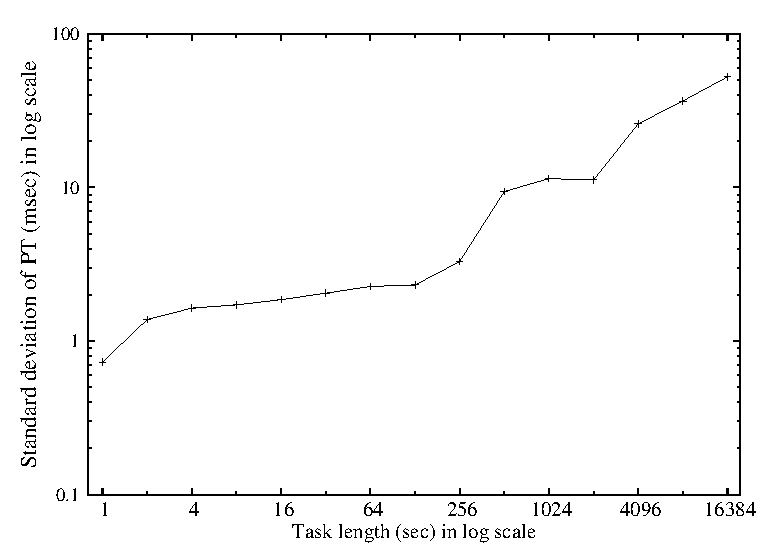
\includegraphics[scale=0.8]{overall_pt_std.eps}
	\caption{Std. dev. of PT over increasing task length~ (See Table~\ref{tab:exp_notes1}.)\label{fig:incr_task_len}}
\end{figure}

\newpage

\section{Histograms on the EMPv4 Data~\label{sec:empv4_hist}}
The base data of the following histograms are from Table~\ref{tab:exp_notes1}.

\begin{figure}[hp!]
	\centering
	\subfigure[PT frequency on PUT1]{
		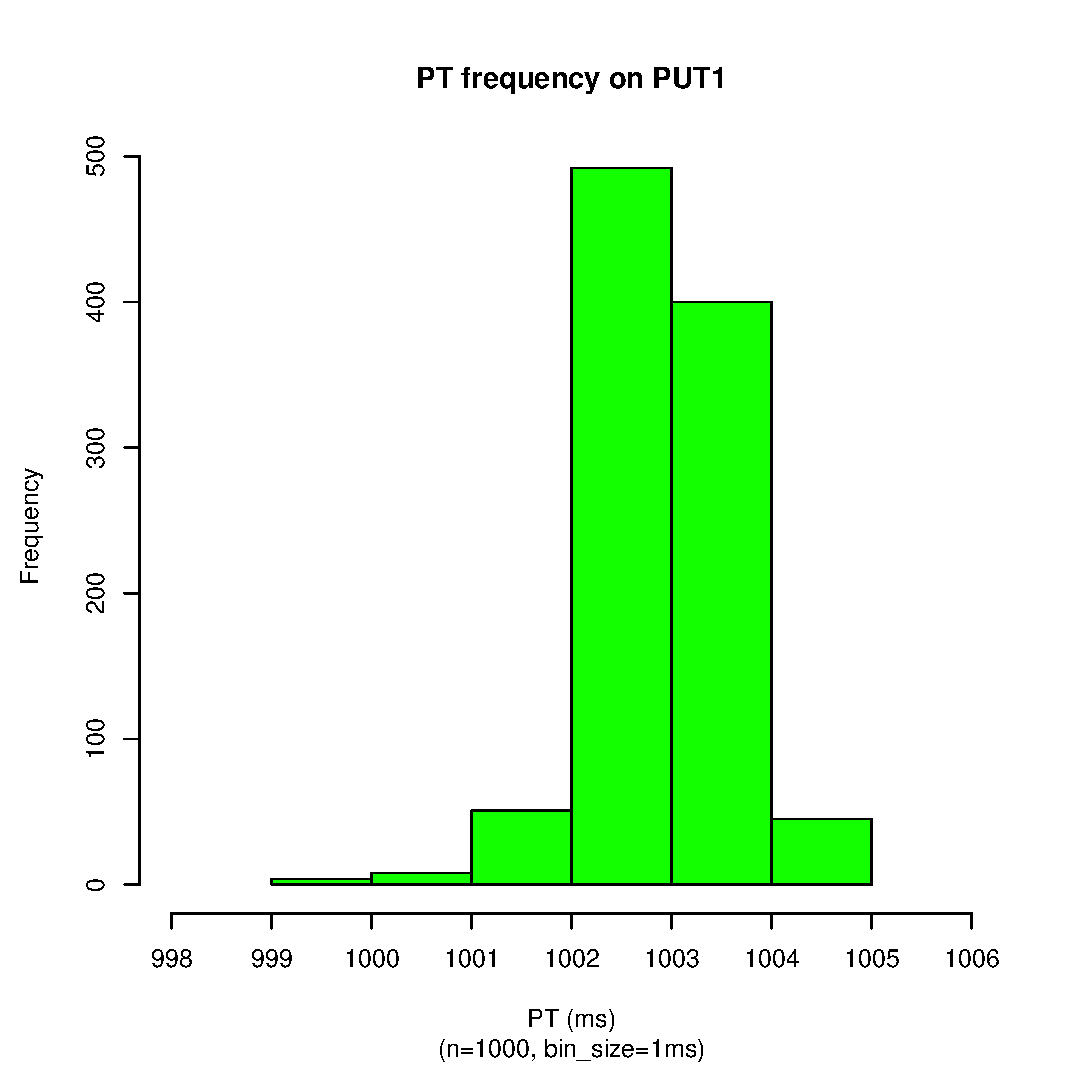
\includegraphics[scale=0.43]{1_sec_pt_hist.eps}
		\label{fig:put1_hist}
	}
	\subfigure[PT frequency on PUT2]{
		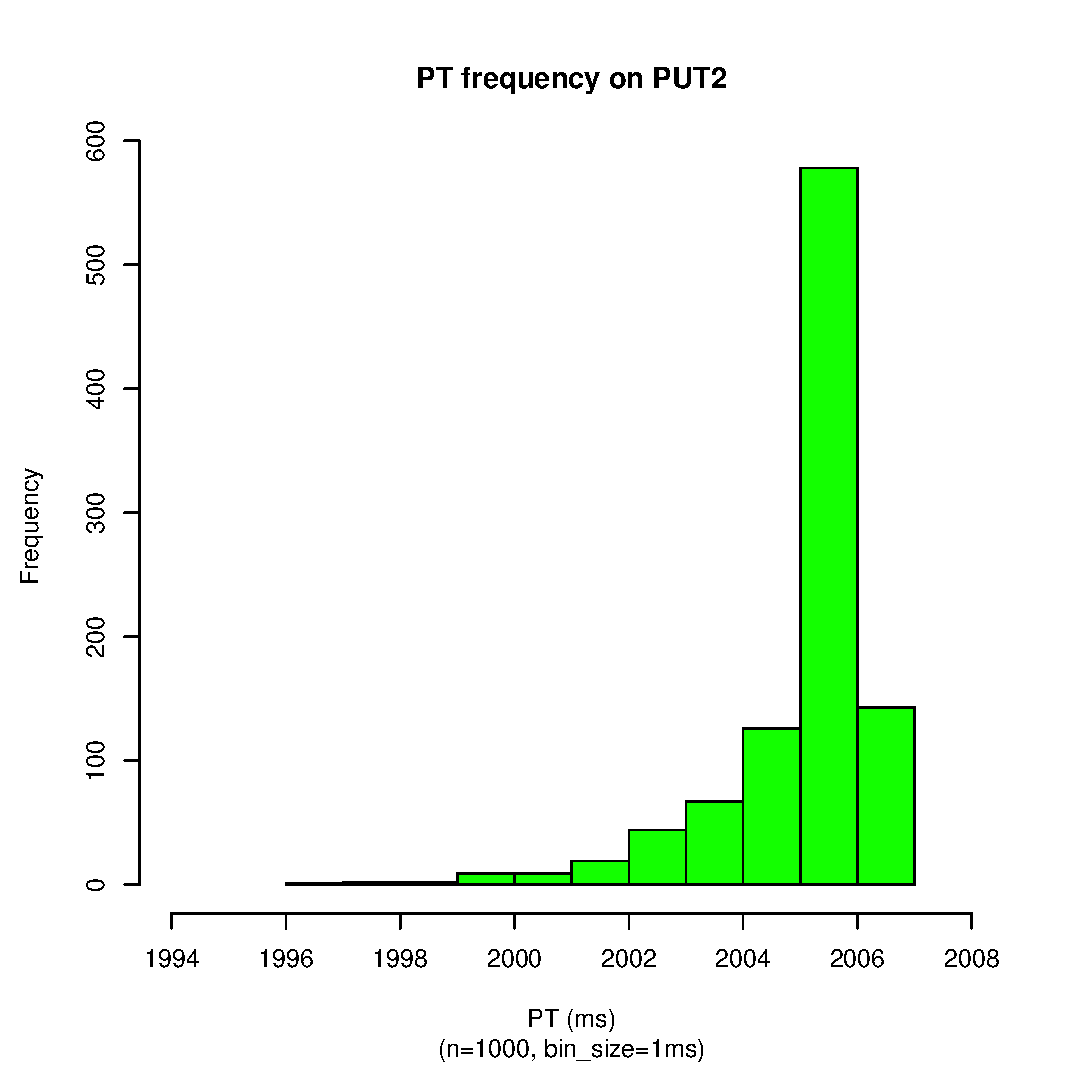
\includegraphics[scale=0.43]{2_sec_pt_hist.eps}
		\label{fig:put2_hist}
	}
	\subfigure[PT frequency on PUT4]{
		\includegraphics[scale=0.43]{4_sec_pt_hist.eps}
		\label{fig:put4_hist}
	}
	\subfigure[PT frequency on PUT8]{
		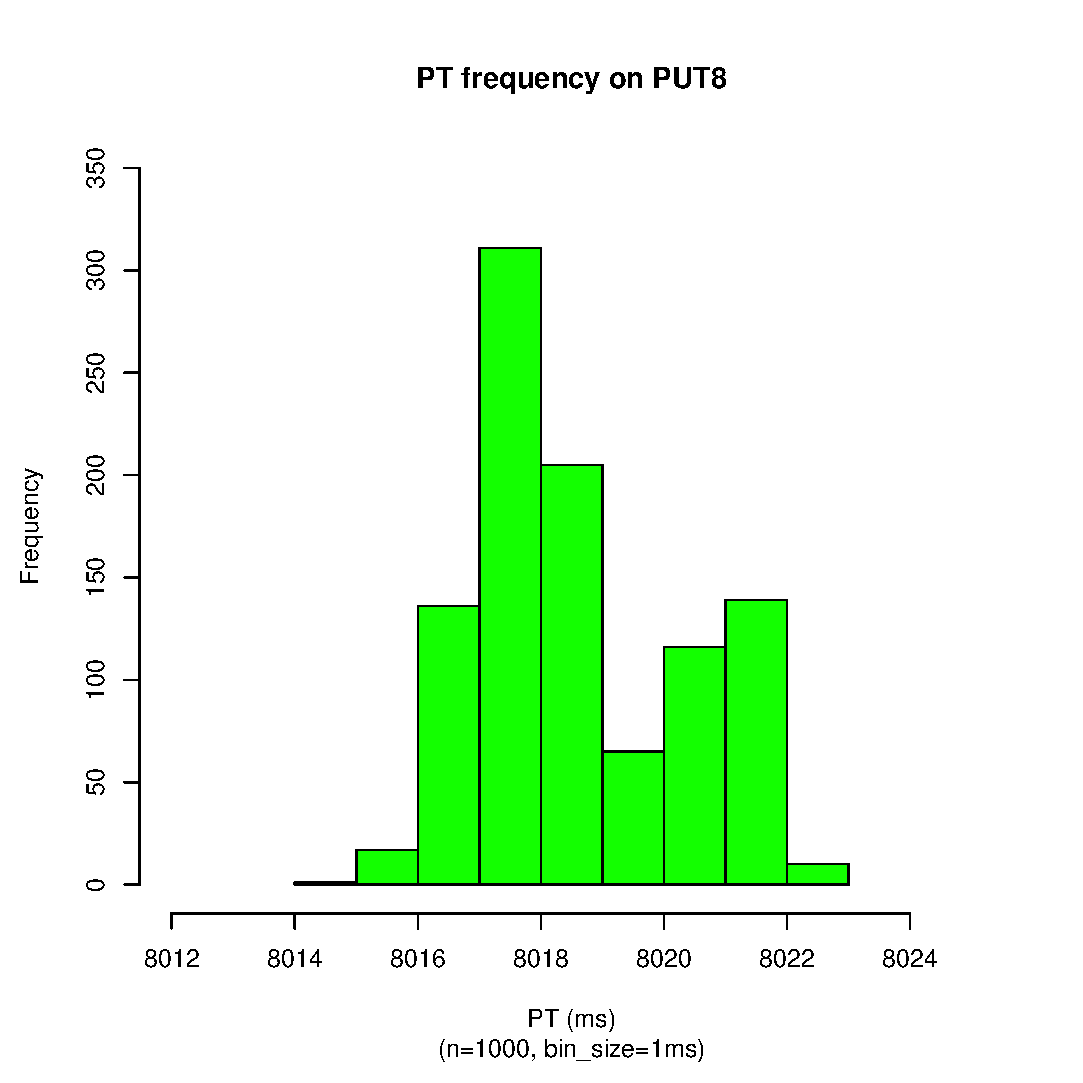
\includegraphics[scale=0.43]{8_sec_pt_hist.eps}
		\label{fig:put8_hist}
	}
	\caption{PT Histograms of PUT1 ... PUT8~\label{fig:pt_hist1}}
\end{figure}

\begin{figure}[hp!]
	\centering
	\subfigure[PT frequency on PUT16]{
		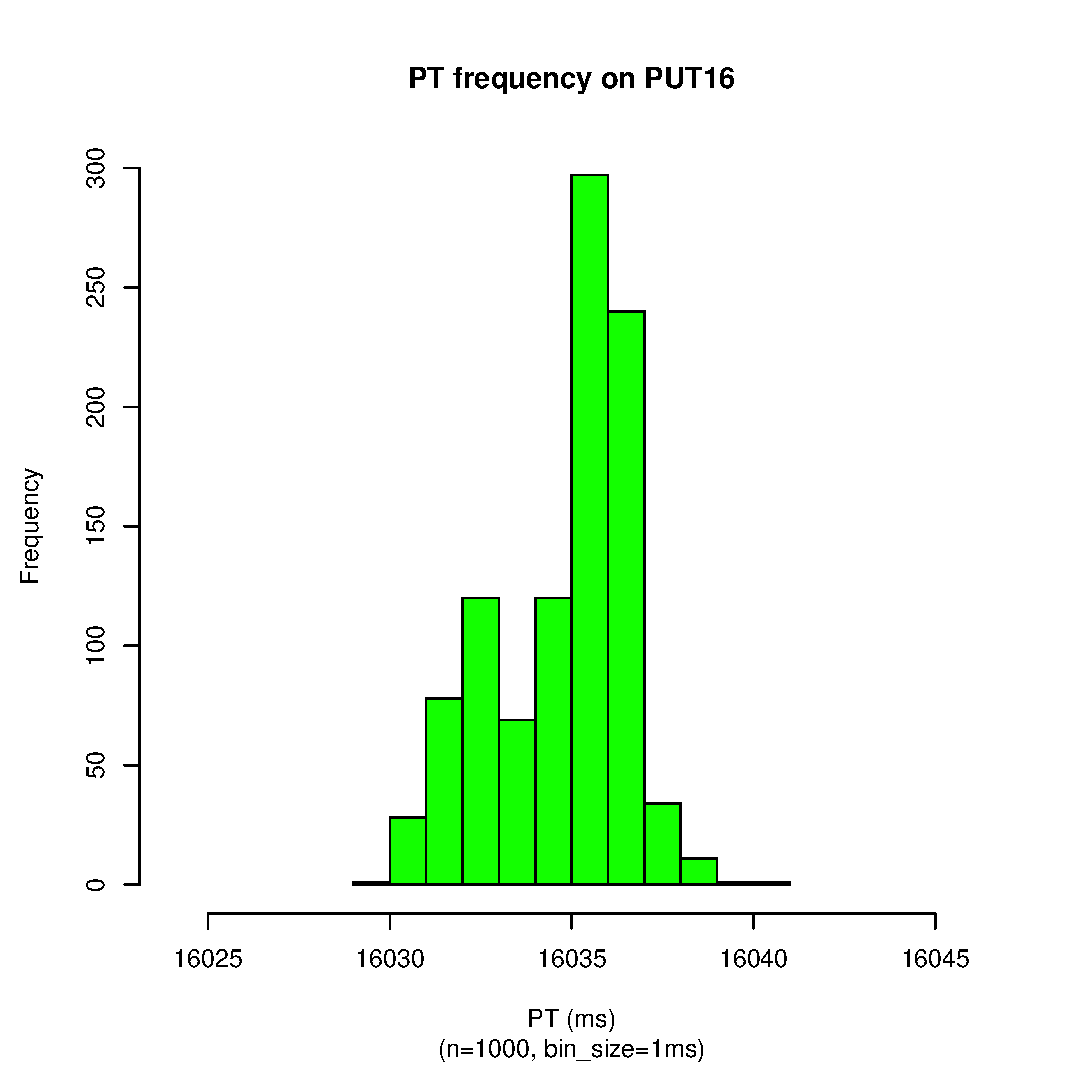
\includegraphics[scale=0.43]{16_sec_pt_hist.eps}
		\label{fig:put16_hist}
	}
	\subfigure[PT frequency on PUT32]{
		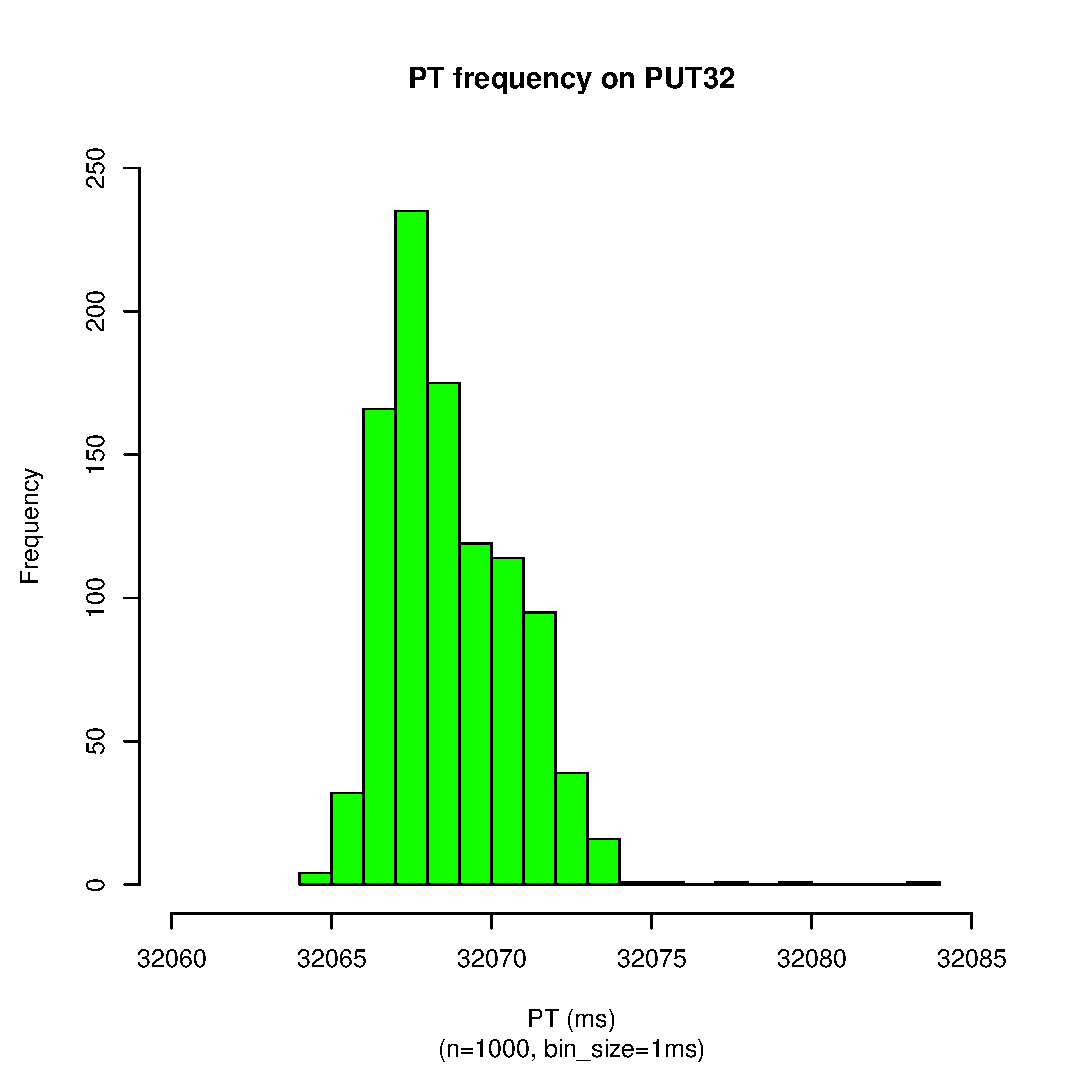
\includegraphics[scale=0.43]{32_sec_pt_hist.eps}
		\label{fig:put32_hist}
	}
	\subfigure[PT frequency on PUT64]{
		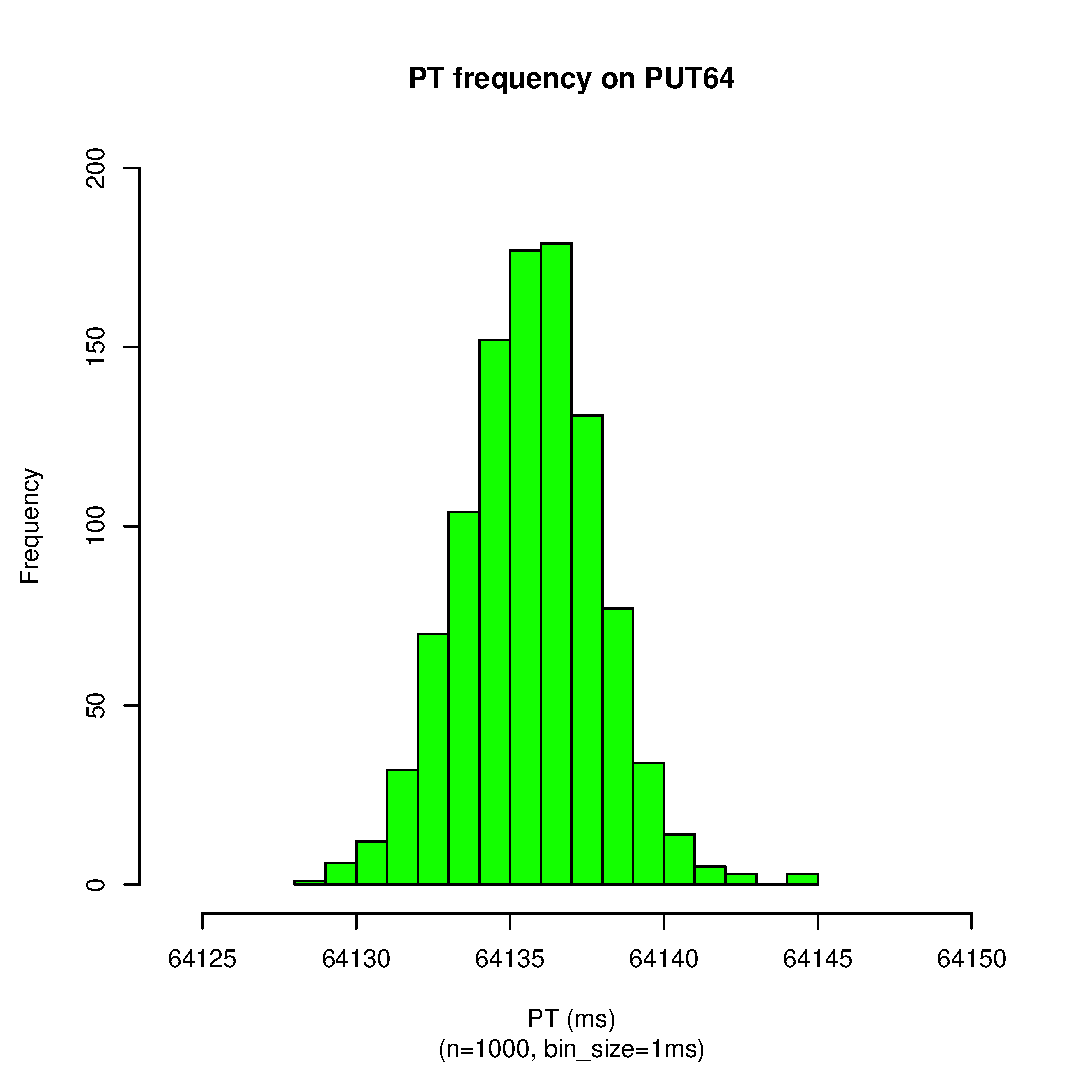
\includegraphics[scale=0.43]{64_sec_pt_hist.eps}
		\label{fig:put64_hist}
	}
	\caption{PT Histograms of PUT16 ... PUT64~\label{fig:pt_hist2}}
\end{figure}

\newpage

\begin{figure}[hp!]
	\centering
	\subfigure[PT frequency on PUT128]{
		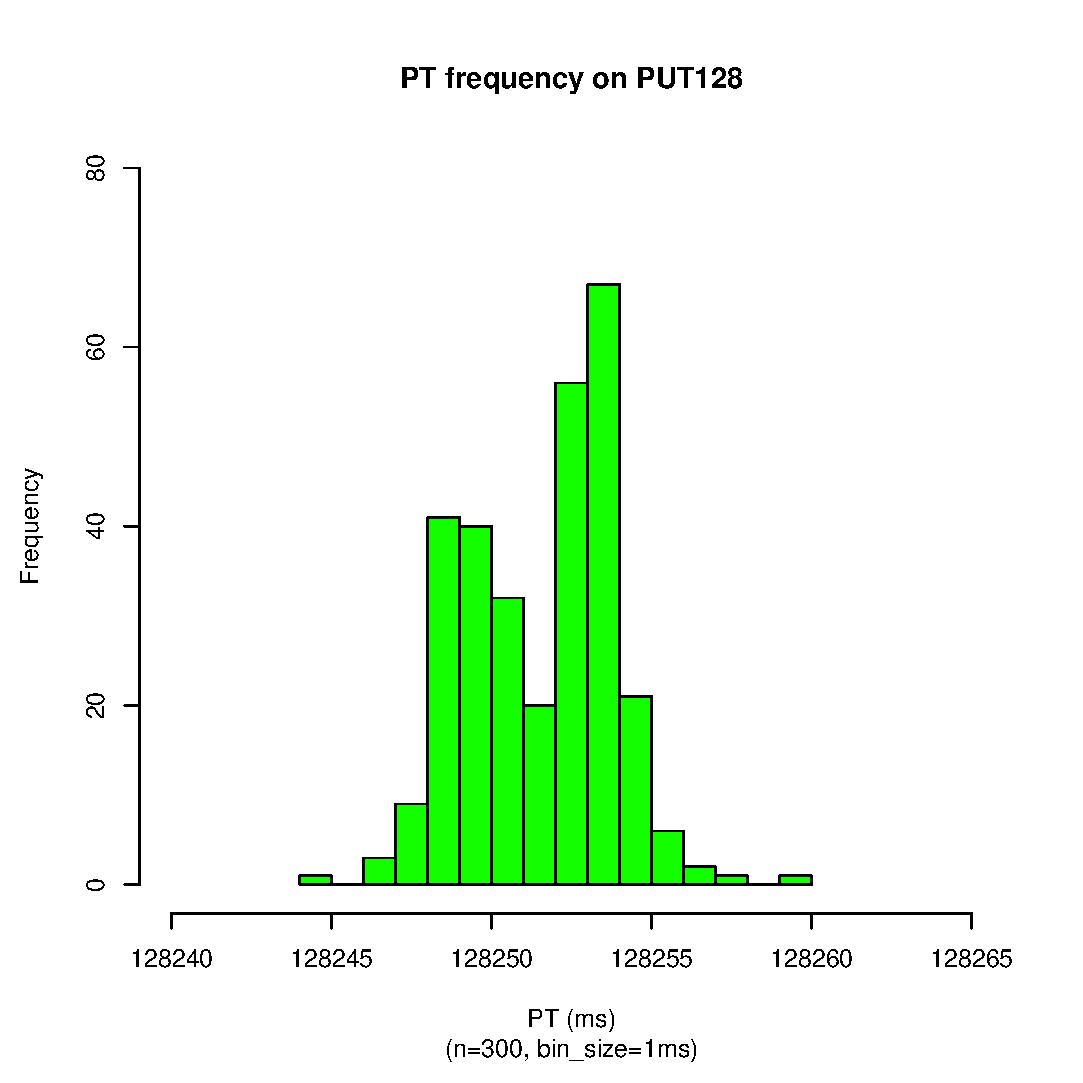
\includegraphics[scale=0.43]{128_sec_pt_hist.eps}
		\label{fig:put128_hist}
	}
	\subfigure[PT frequency on PUT256]{
		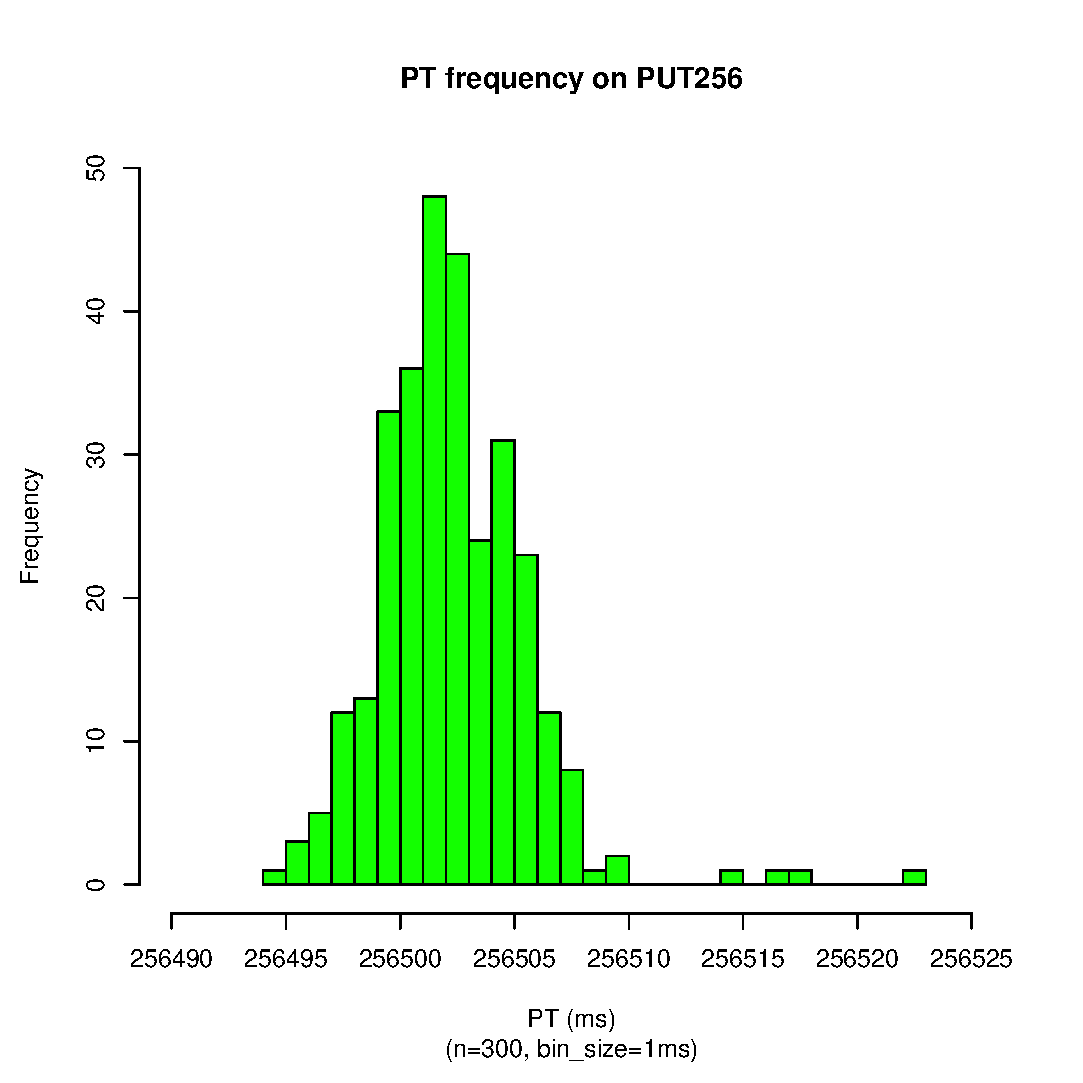
\includegraphics[scale=0.43]{256_sec_pt_hist.eps}
		\label{fig:put256_hist}
	}
	\subfigure[PT frequency on PUT512]{
		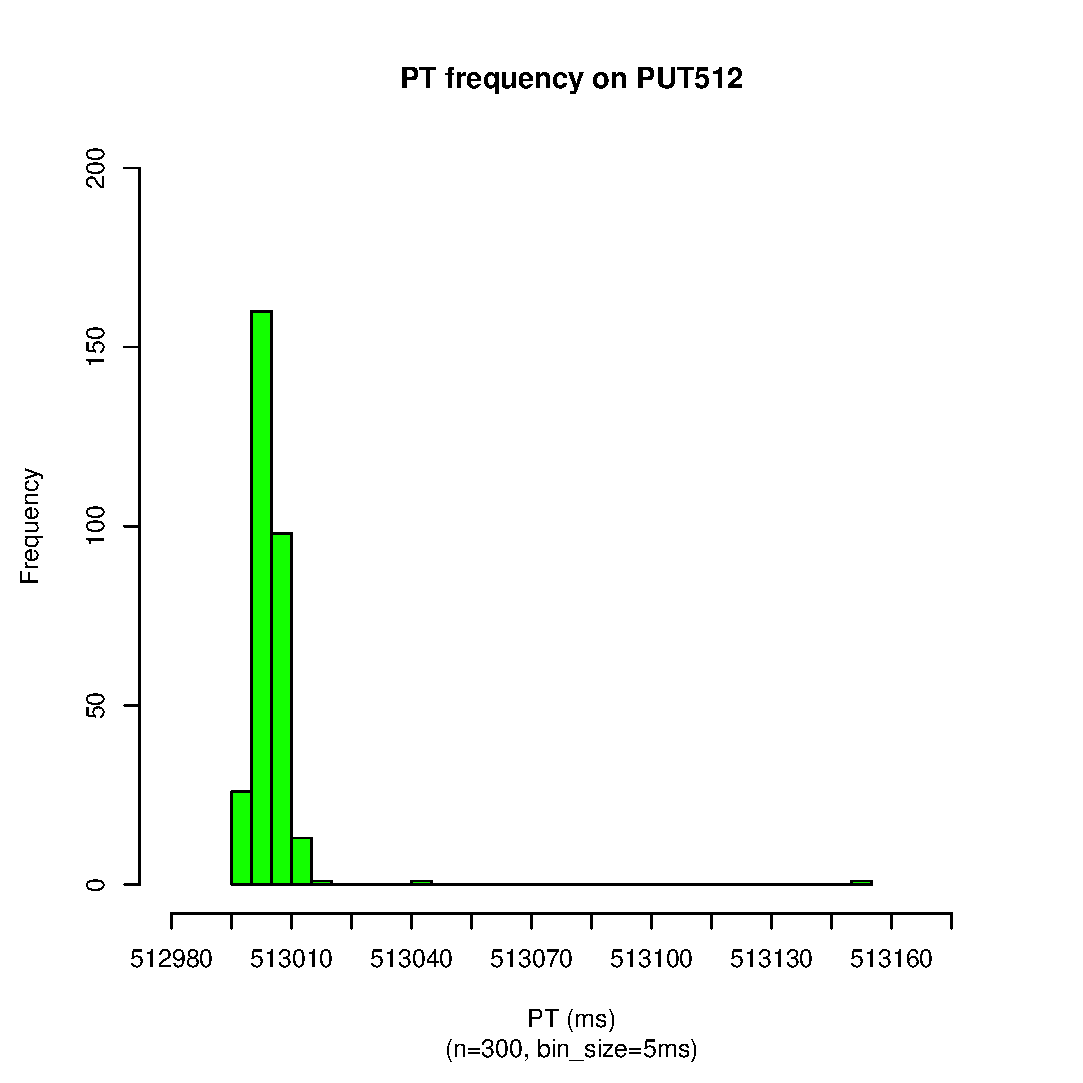
\includegraphics[scale=0.43]{512_sec_pt_hist.eps}
		\label{fig:put512_hist}
	}
	\subfigure[PT frequency on PUT1024]{
		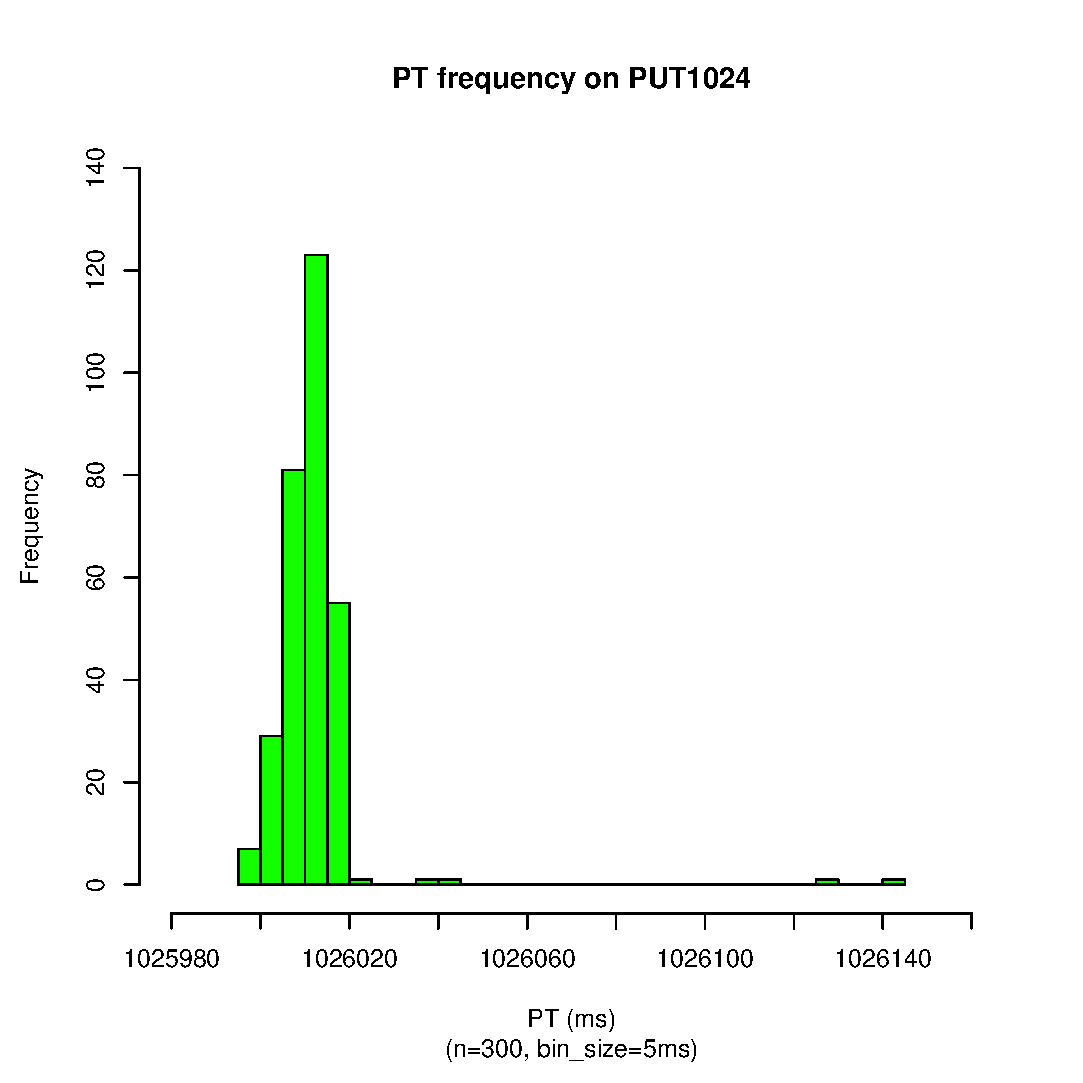
\includegraphics[scale=0.43]{1024_sec_pt_hist.eps}
		\label{fig:put1024_hist}
	}
	\caption{PT Histograms of PUT128 ... PUT1024~\label{fig:pt_hist3}}
\end{figure}

\newpage

\begin{figure}[hp!]
	\centering
	\subfigure[PT frequency on PUT2048]{
		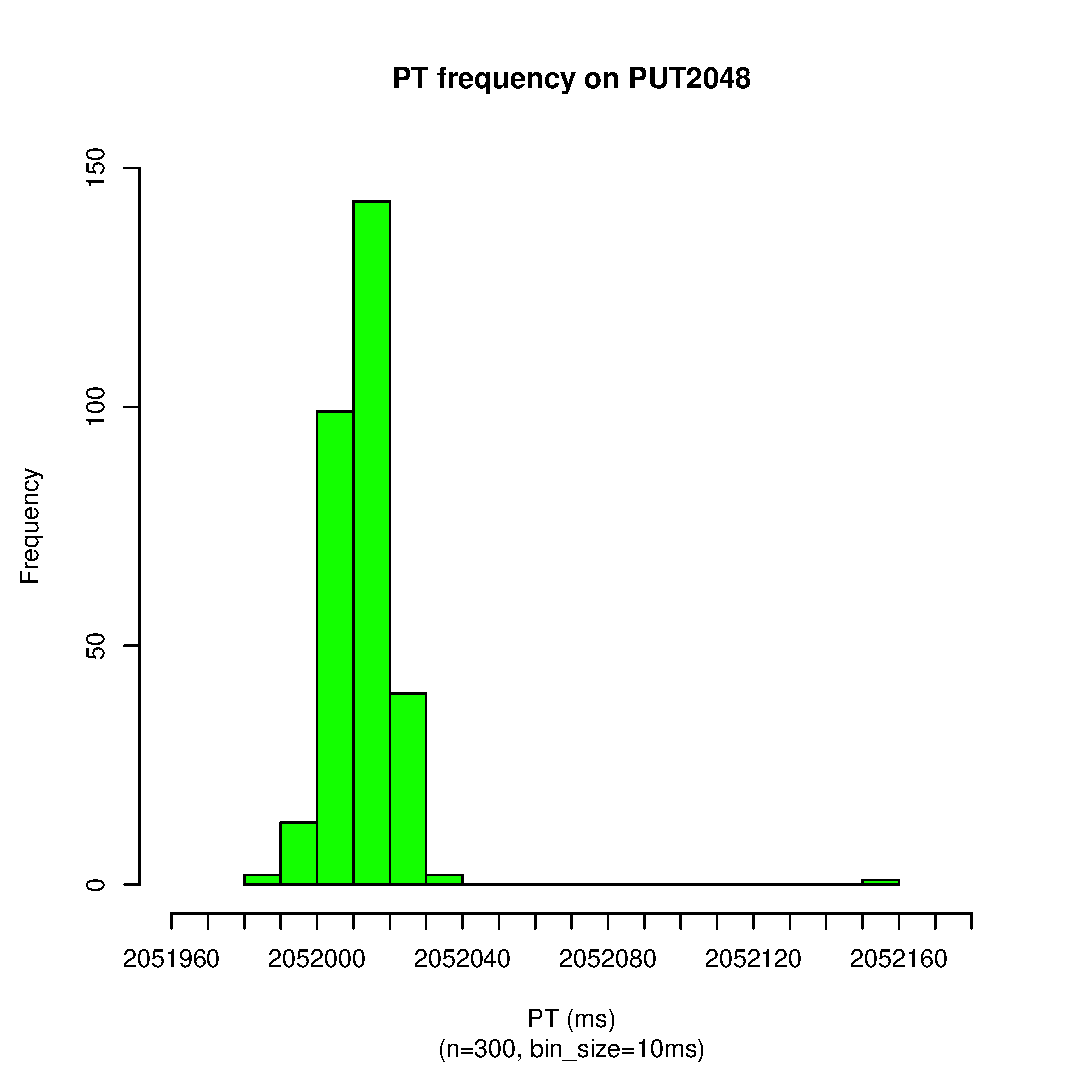
\includegraphics[scale=0.43]{2048_sec_pt_hist.eps}
		\label{fig:put2048_hist}
	}
	\subfigure[PT frequency on PUT4096]{
		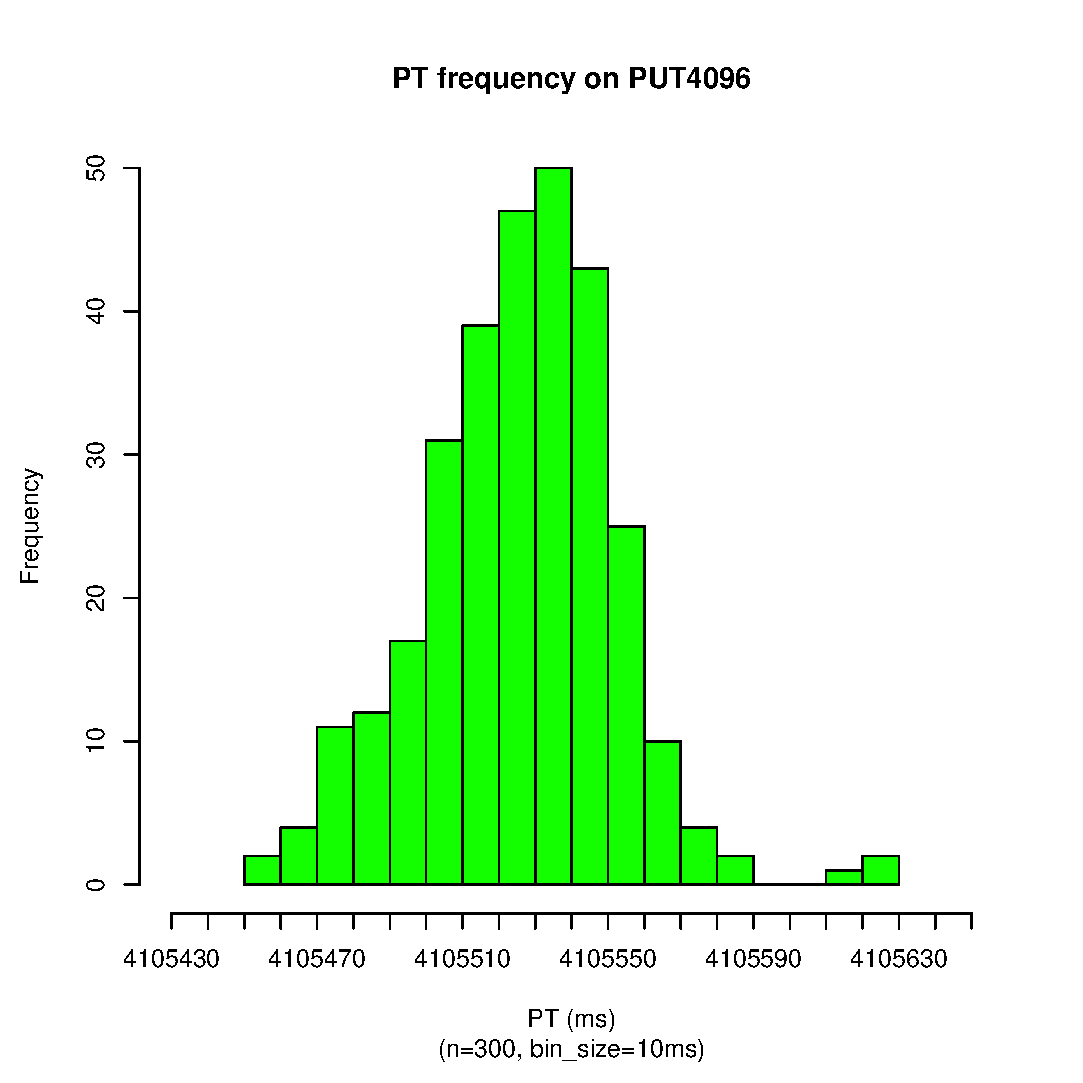
\includegraphics[scale=0.43]{4096_sec_pt_hist.eps}
		\label{fig:put4096_hist}
	}
	\caption{PT Histograms of PUT2048 and PUT4096~\label{fig:pt_hist4}}
\end{figure}


\newpage

\begin{figure}[hp!]
	\centering
	\subfigure[PT frequency on PUT8192 with 40 samples  (See Table~\ref{tab:exp_notes1}.)]{
		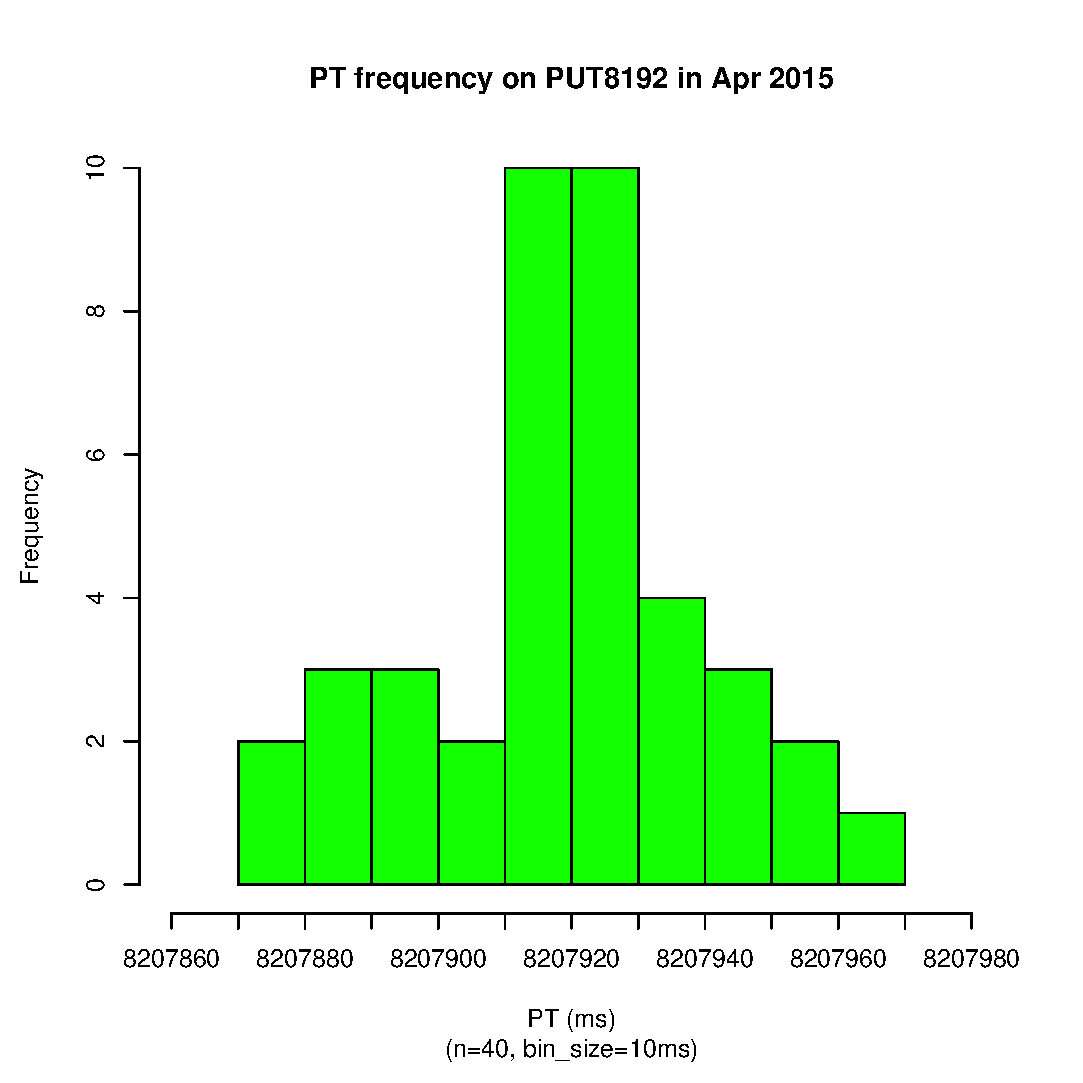
\includegraphics[scale=0.43]{8192_sec_pt_hist1.eps}
		\label{fig:put8192_hist1}
	}
	\subfigure[PT frequency on PUT8192 with 260 samples (See Table~\ref{tab:exp_notes1}.)]{
		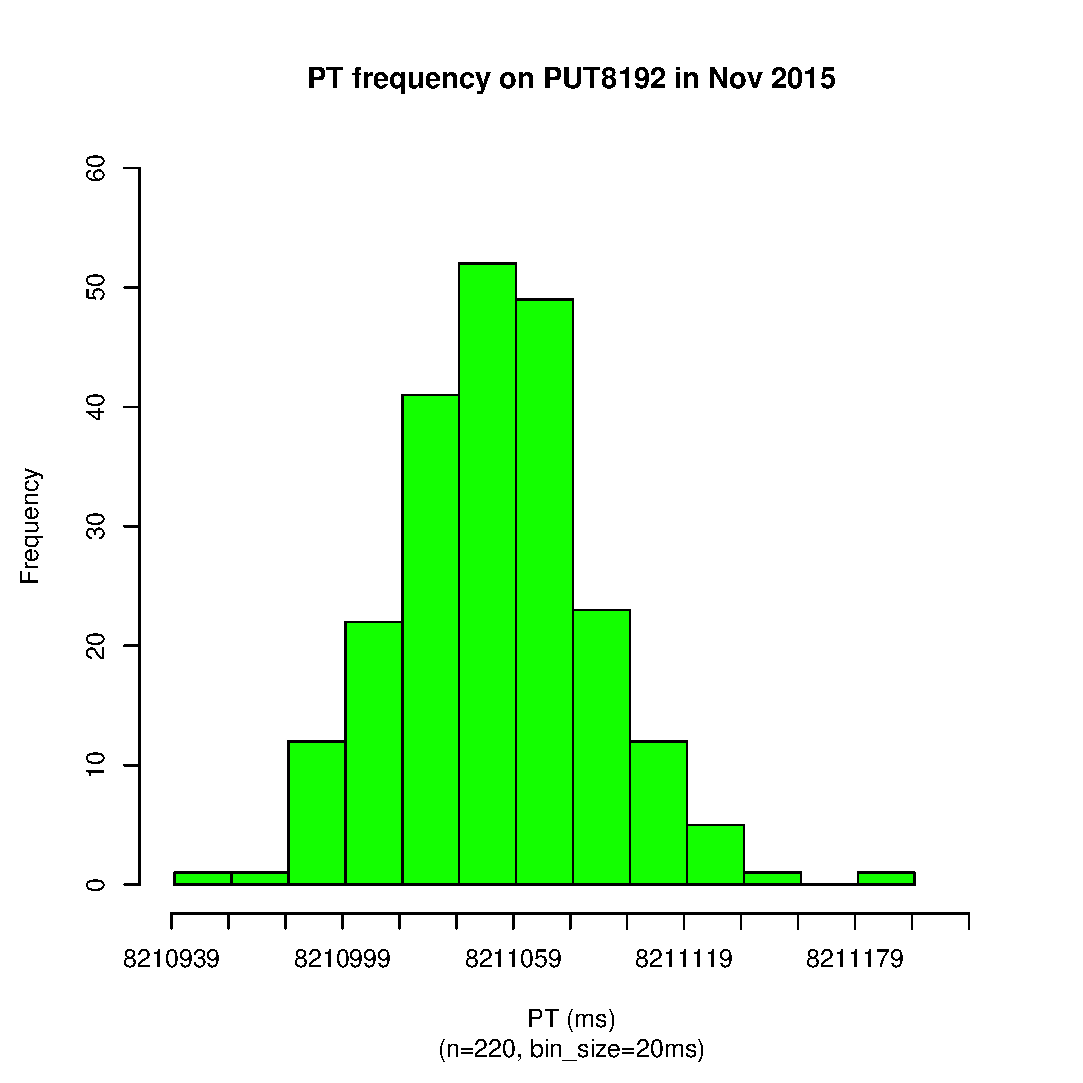
\includegraphics[scale=0.43]{8192_sec_pt_hist2.eps}
		\label{fig:put8192_hist2}
	}
	\subfigure[PT frequency on PUT16384 with 40 samples (See Table~\ref{tab:exp_notes1}.)]{
		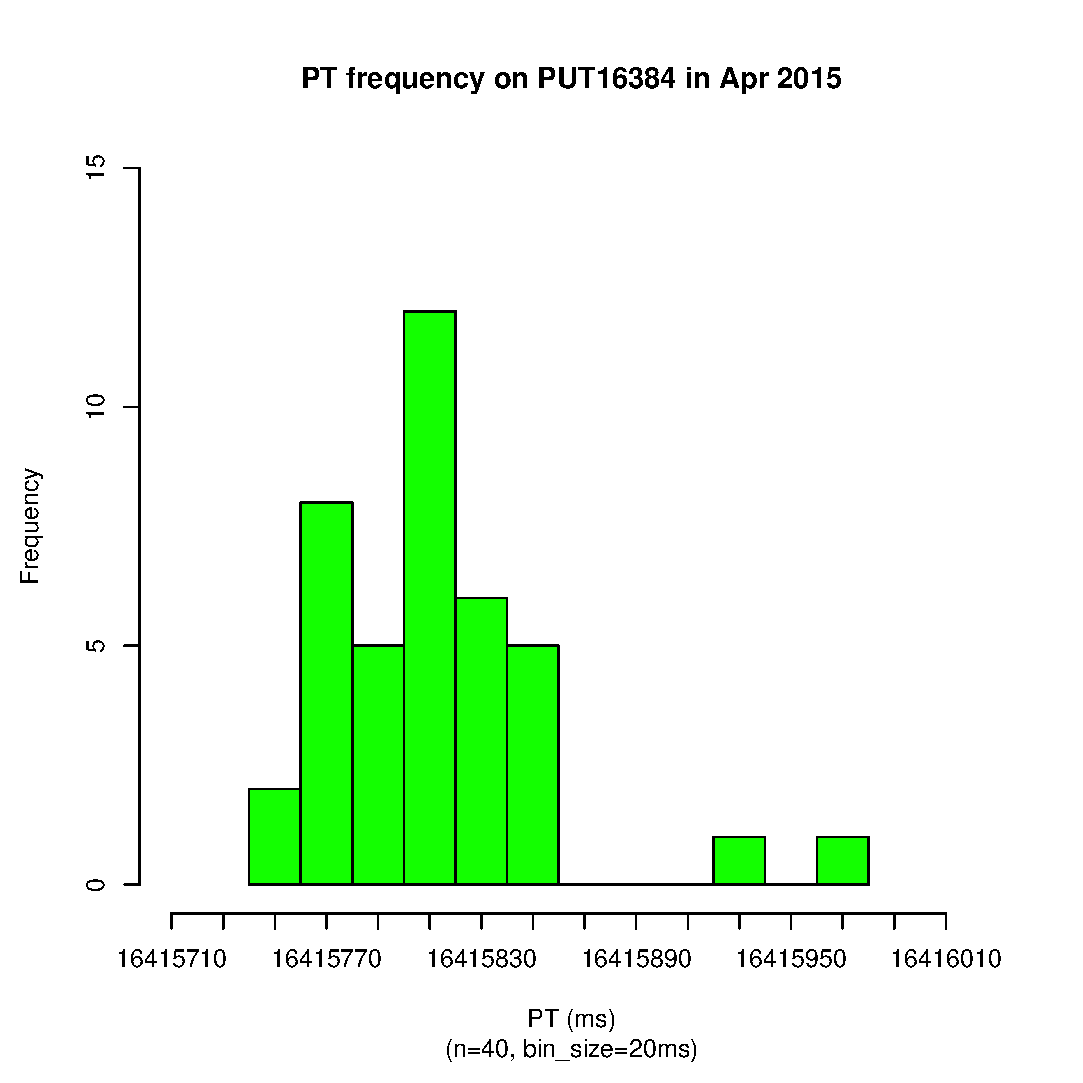
\includegraphics[scale=0.43]{16384_sec_pt_hist1.eps}
		\label{fig:put16384_hist1}
	}
	\subfigure[PT frequency on PUT16384 with 260 samples (See Table~\ref{tab:exp_notes1}.)]{
		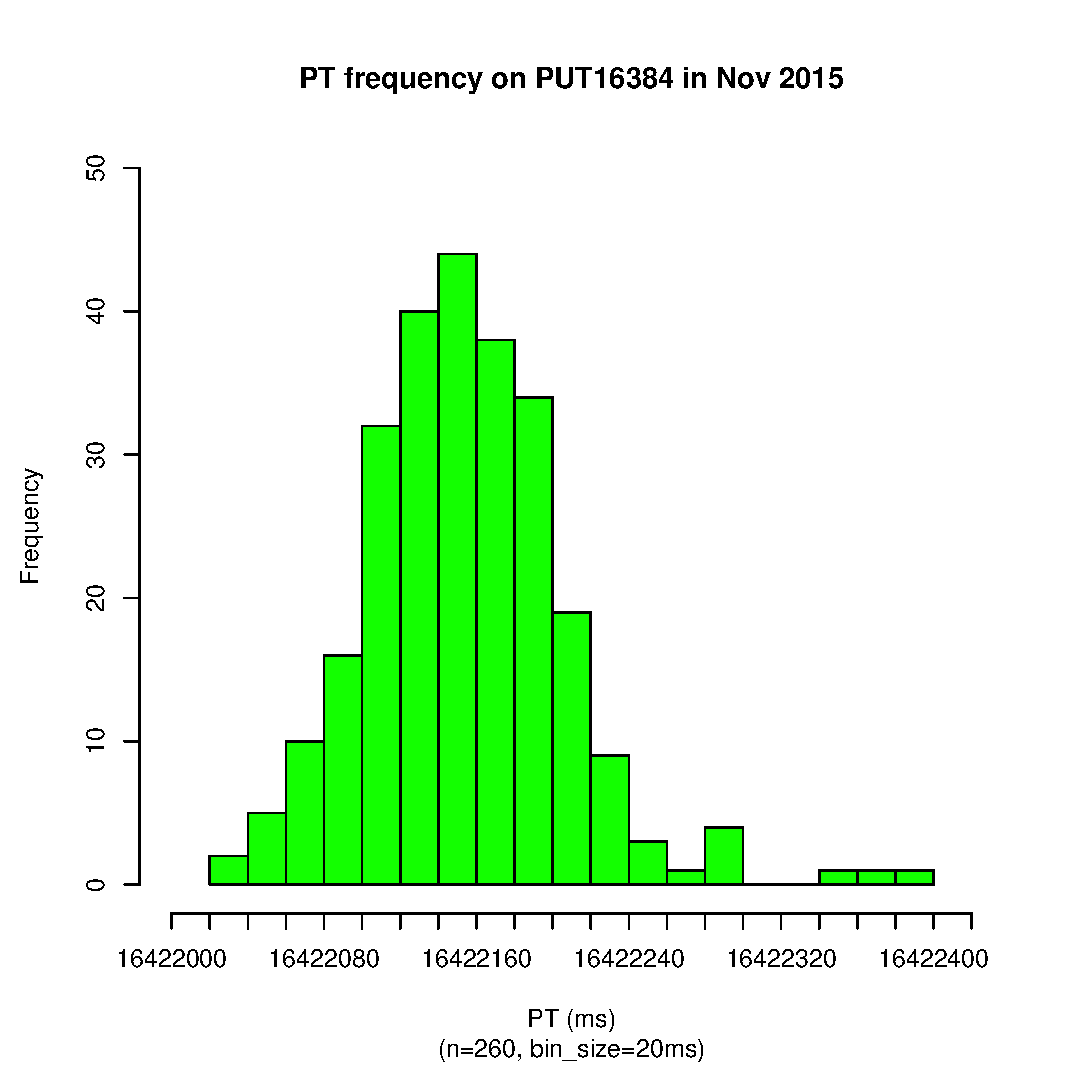
\includegraphics[scale=0.43]{16384_sec_pt_hist2.eps}
		\label{fig:put16384_hist2}
	}
	\caption{PT Histograms of PUT8192 and PUT16384~\label{fig:pt_hist5}}
\end{figure}

\newpage

\section{Histograms on the EMPv5 Data~\label{sec:empv5_hist}}
The base data of the following histograms are from Table~\ref{tab:exp_notes1}. 
EMPv5(-relaxed) trims outliers from the data of each PUT by EMPv4.
To be more specific, for each run of PUT an outlier is determined 
as the one above and below the average $\pm$ *five\footnote{In the stricter version, we use *two*.}* 
standard deviations computed from the EMPv4 data.

\begin{figure}[hp!]
	\centering
	\subfigure[PT frequency on PUT1]{
		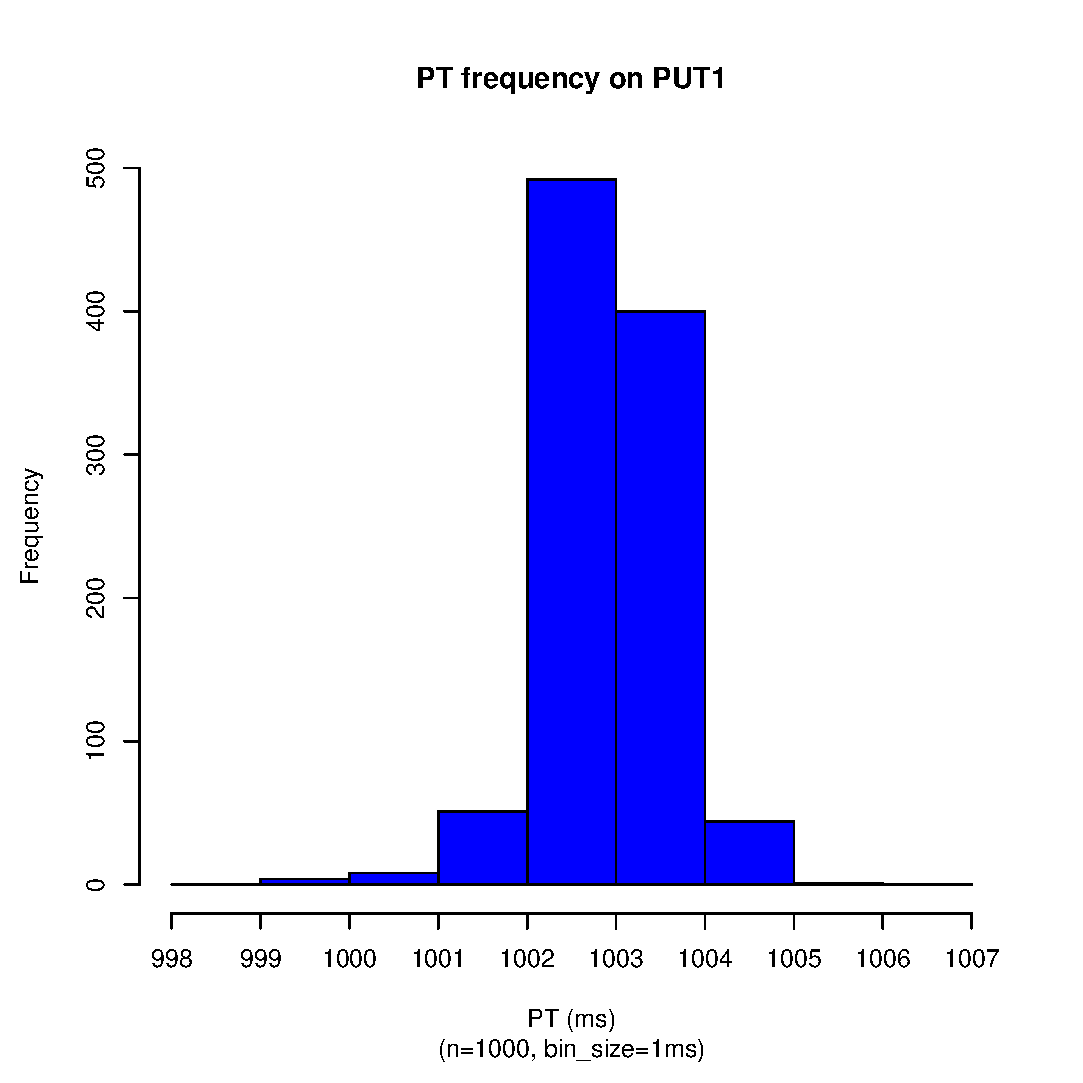
\includegraphics[scale=0.43]{1_sec_pt_hist2.eps}
		\label{fig:put1_hist2}
	}
	\subfigure[PT frequency on PUT2]{
		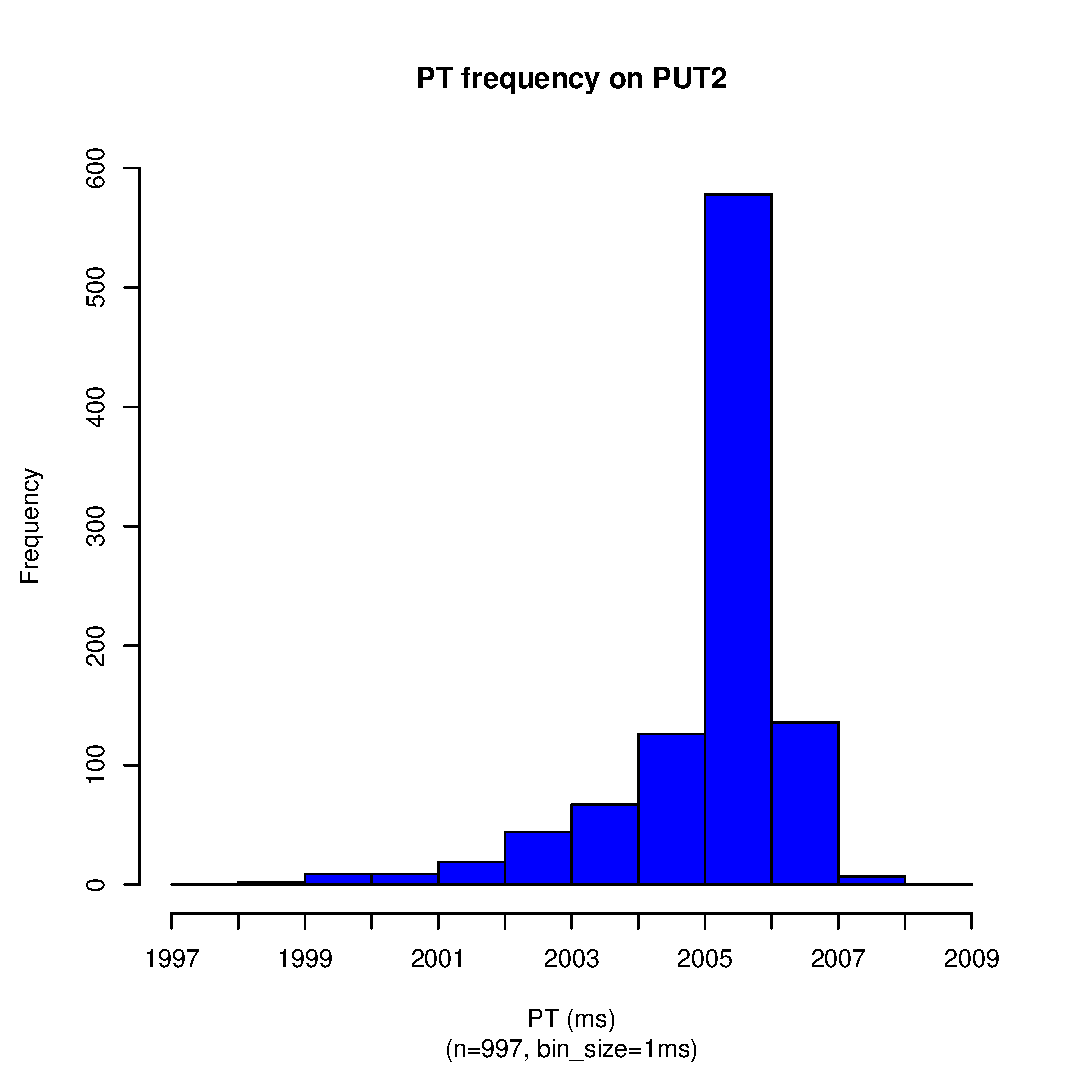
\includegraphics[scale=0.43]{2_sec_pt_hist2.eps}
		\label{fig:put2_hist2}
	}
	\subfigure[PT frequency on PUT4]{
		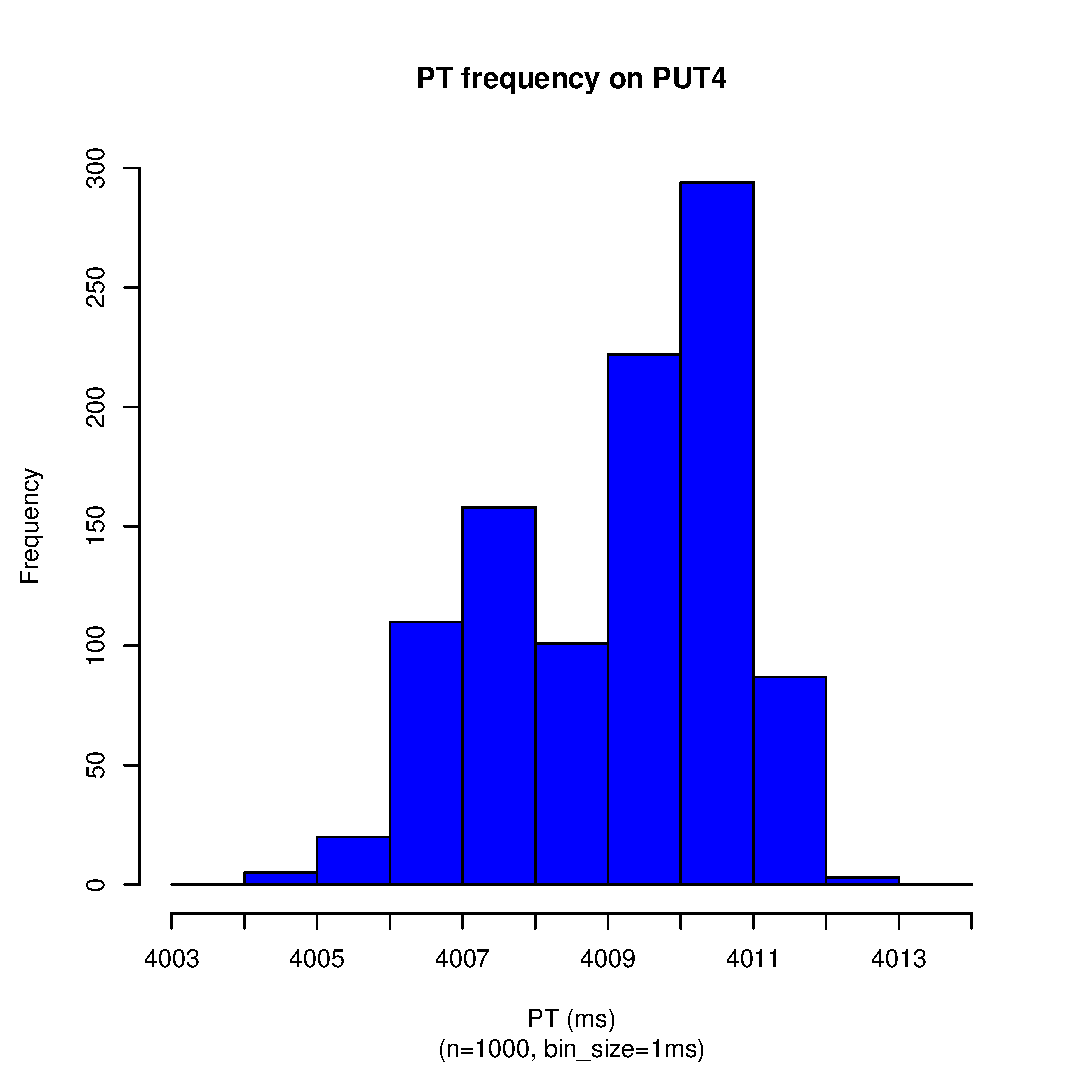
\includegraphics[scale=0.43]{4_sec_pt_hist2.eps}
		\label{fig:put4_hist2}
	}
	\subfigure[PT frequency on PUT8]{
		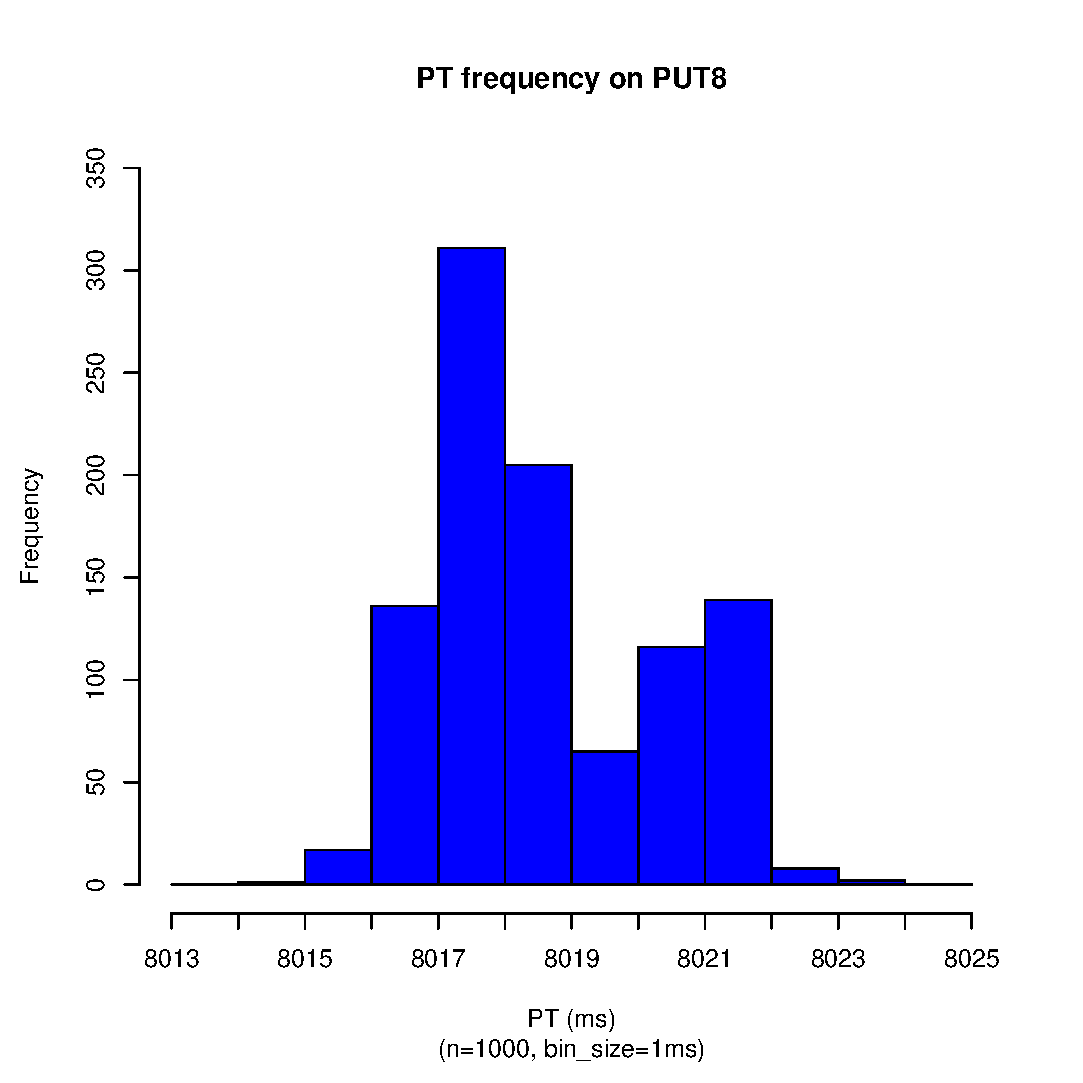
\includegraphics[scale=0.43]{8_sec_pt_hist2.eps}
		\label{fig:put8_hist2}
	}
	\caption{PT Histograms of PUT1 ... PUT8~\label{fig:pt_out_hist1}}
\end{figure}

\newpage

\begin{figure}[hp!]
	\centering
	\subfigure[PT frequency on PUT16]{
		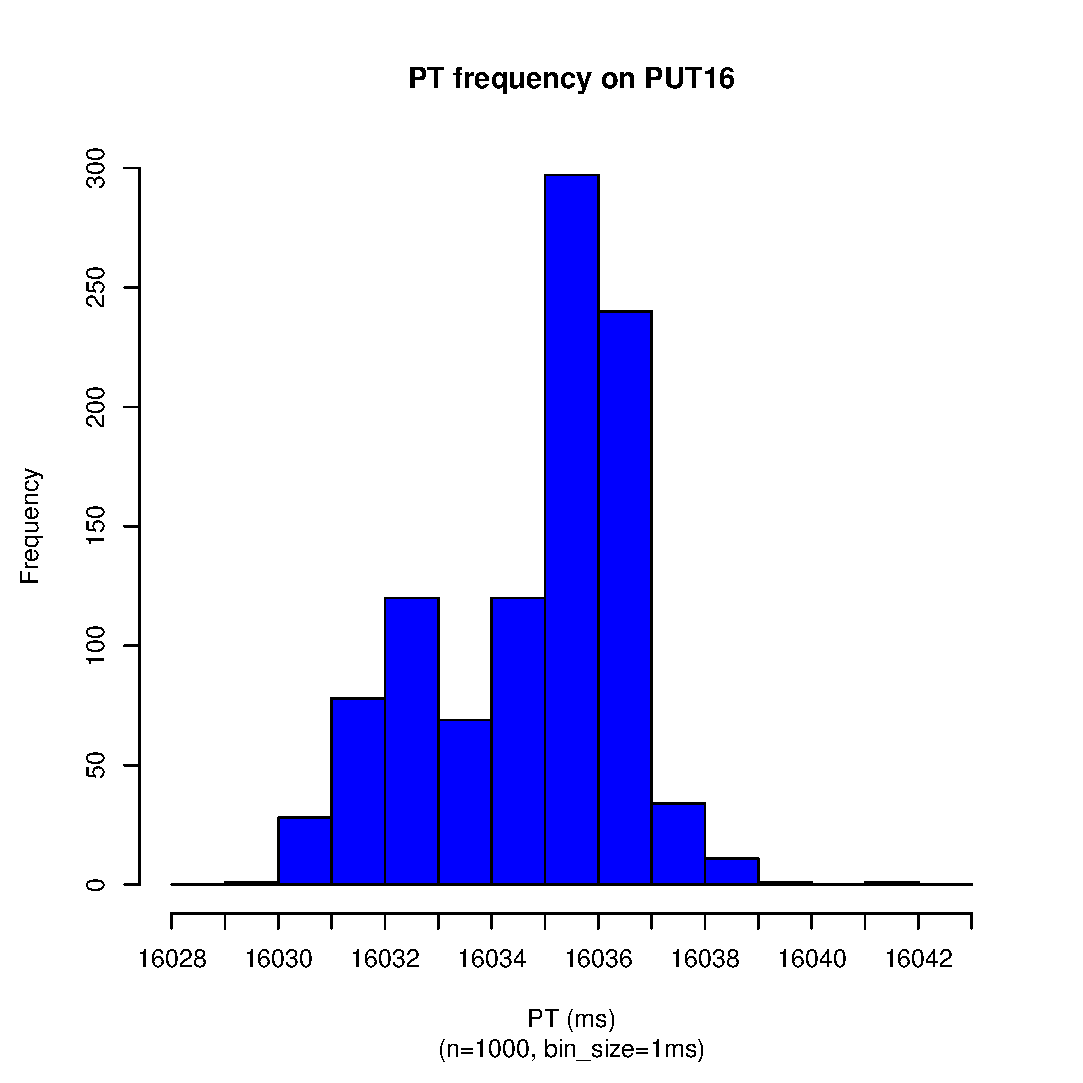
\includegraphics[scale=0.43]{16_sec_pt_hist2.eps}
		\label{fig:put16_hist2}
	}
	\subfigure[PT frequency on PUT32]{
		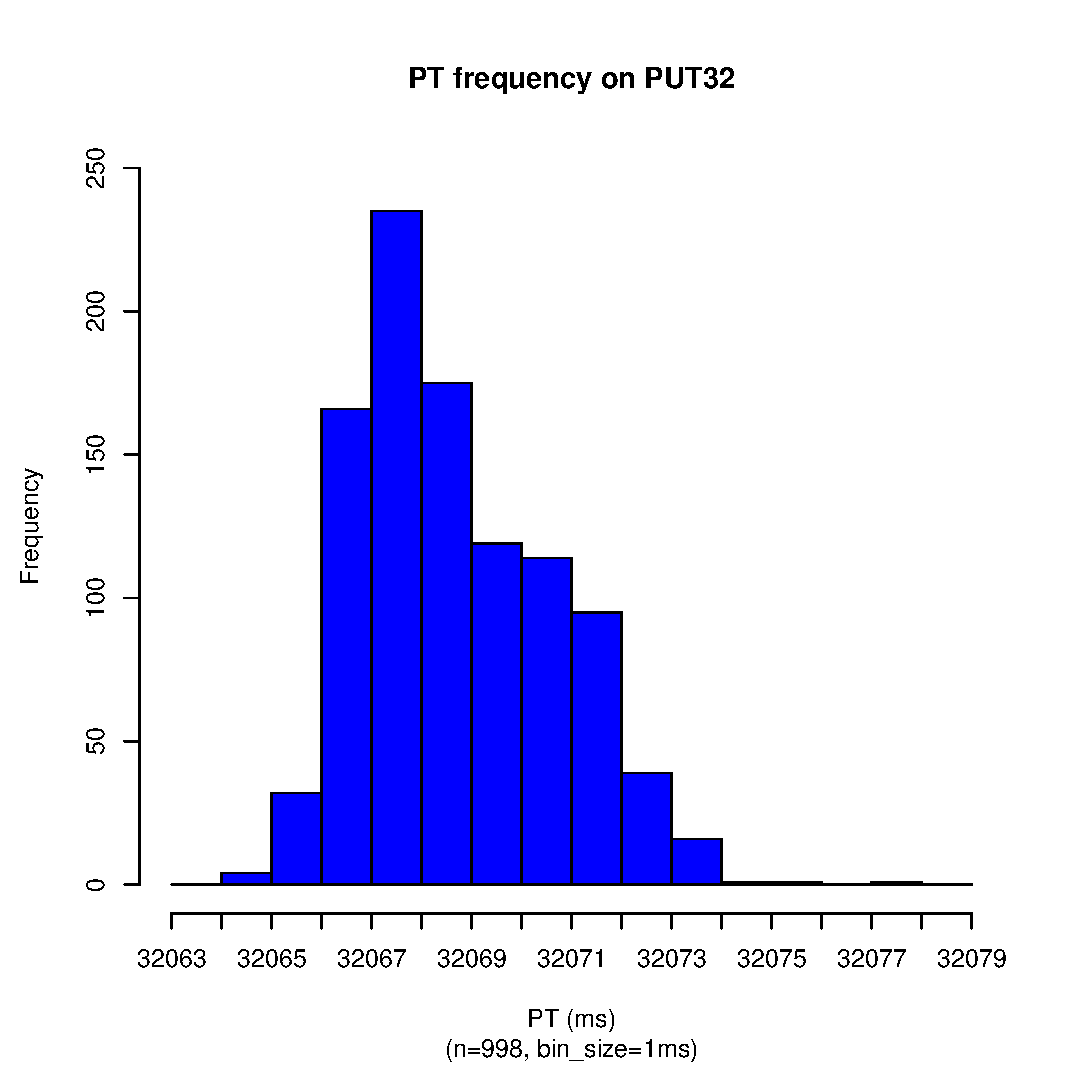
\includegraphics[scale=0.43]{32_sec_pt_hist2.eps}
		\label{fig:put32_hist2}
	}
	\subfigure[PT frequency on PUT64]{
		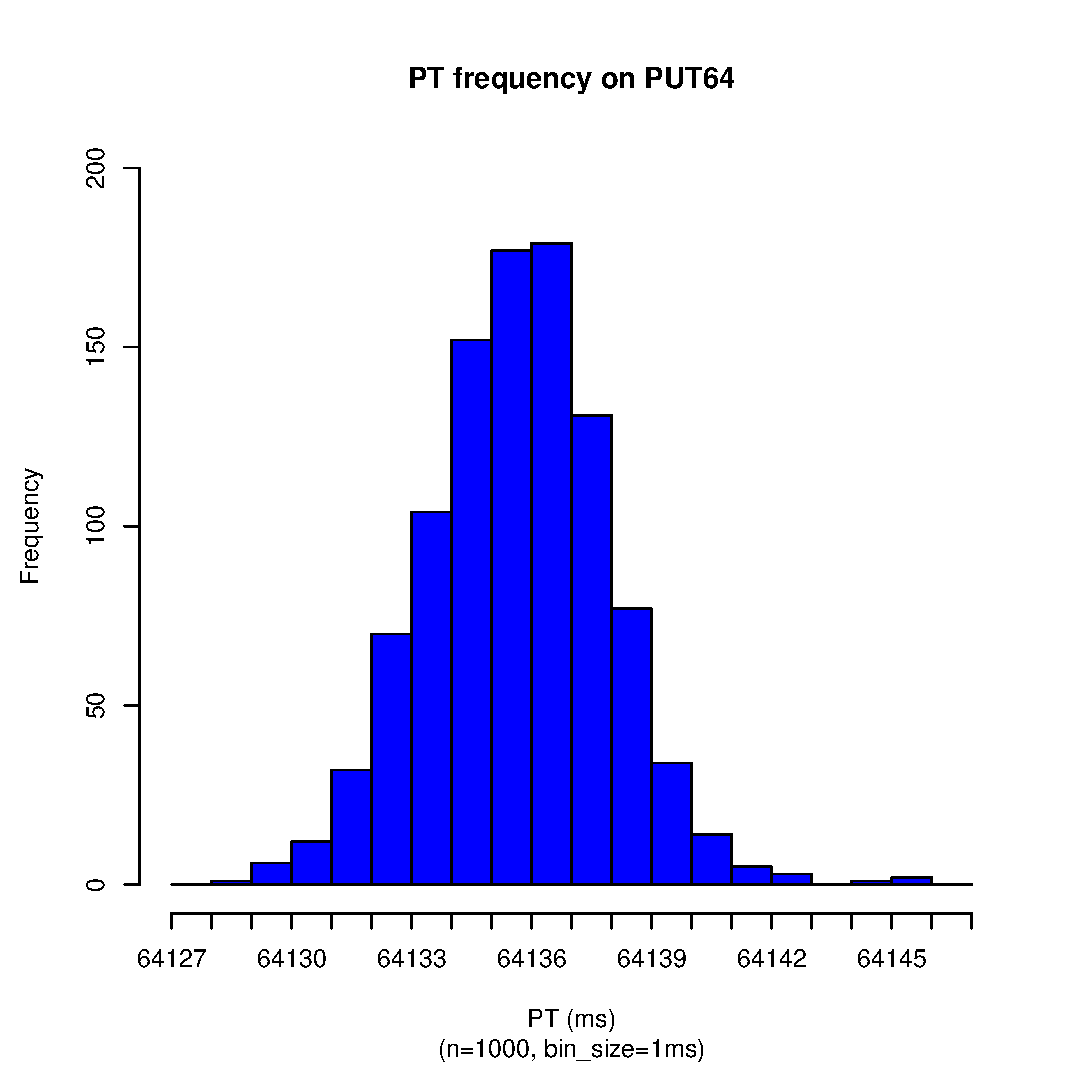
\includegraphics[scale=0.43]{64_sec_pt_hist2.eps}
		\label{fig:put64_hist2}
	}
	\caption{PT Histograms of PUT16 ... PUT64~\label{fig:pt_out_hist2}}
\end{figure}

\begin{figure}[hp!]
	\centering
	\subfigure[PT frequency on PUT128]{
		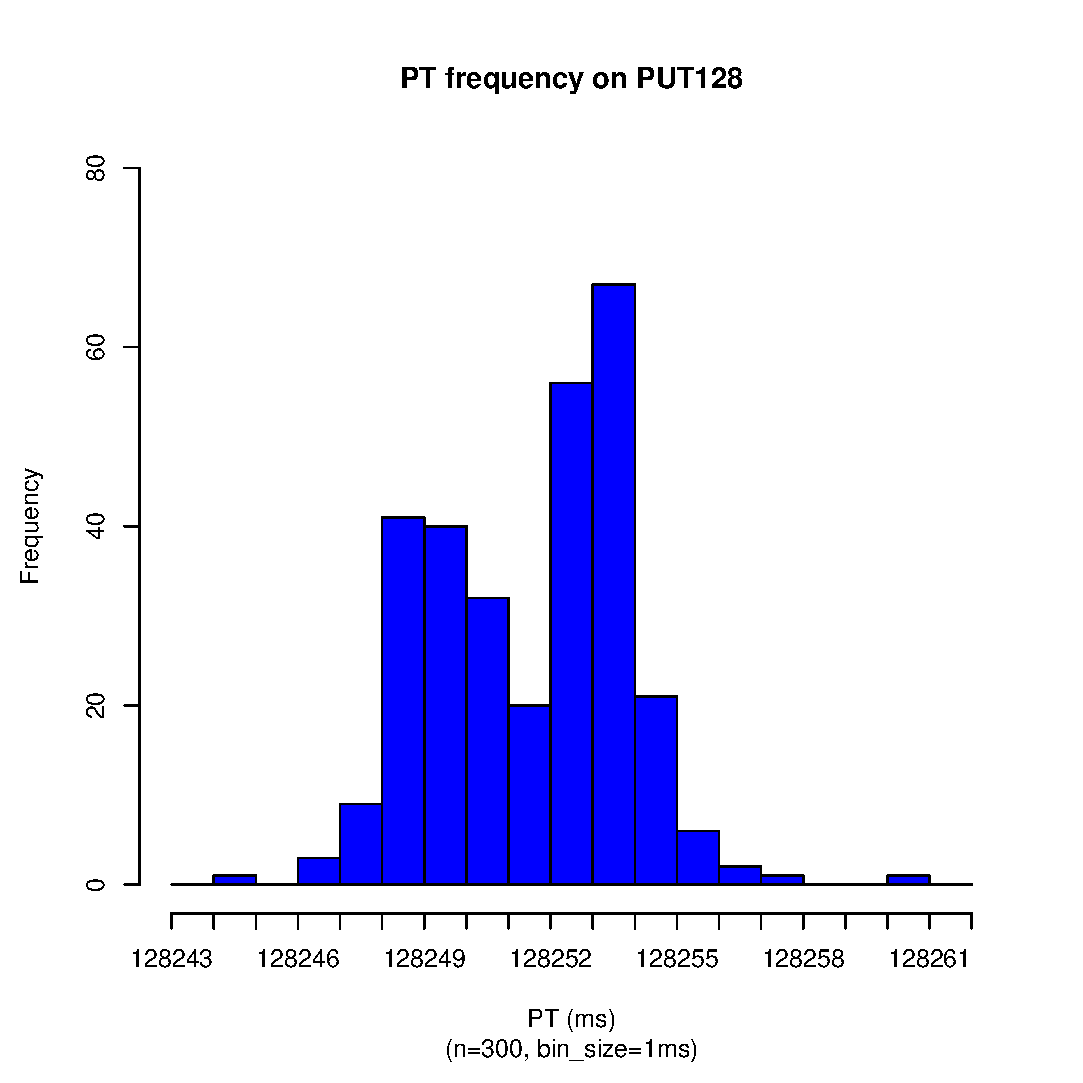
\includegraphics[scale=0.43]{128_sec_pt_hist2.eps}
		\label{fig:put128_hist2}
	}
	\subfigure[PT frequency on PUT256]{
		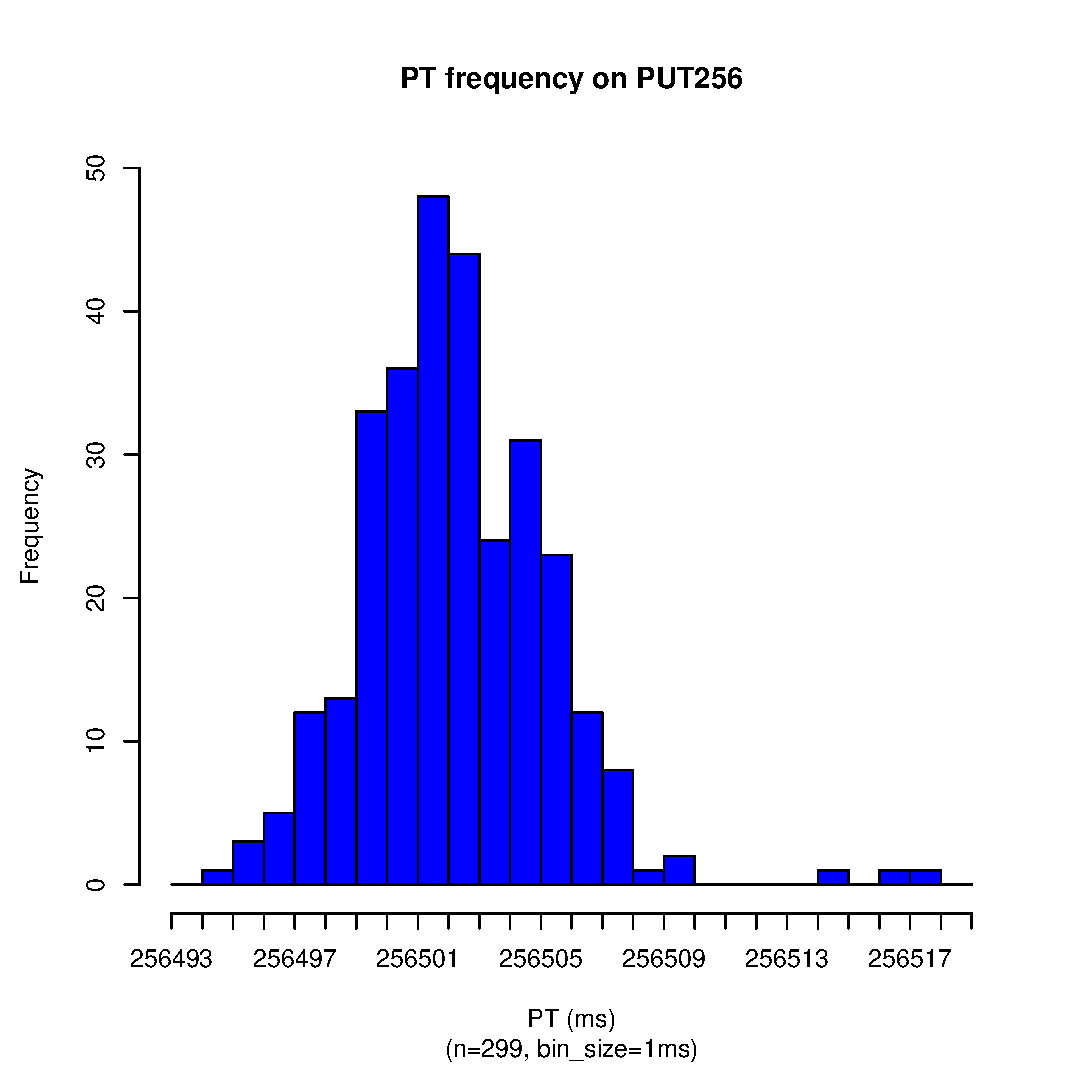
\includegraphics[scale=0.43]{256_sec_pt_hist2.eps}
		\label{fig:put256_hist2}
	}
	\subfigure[PT frequency on PUT512]{
		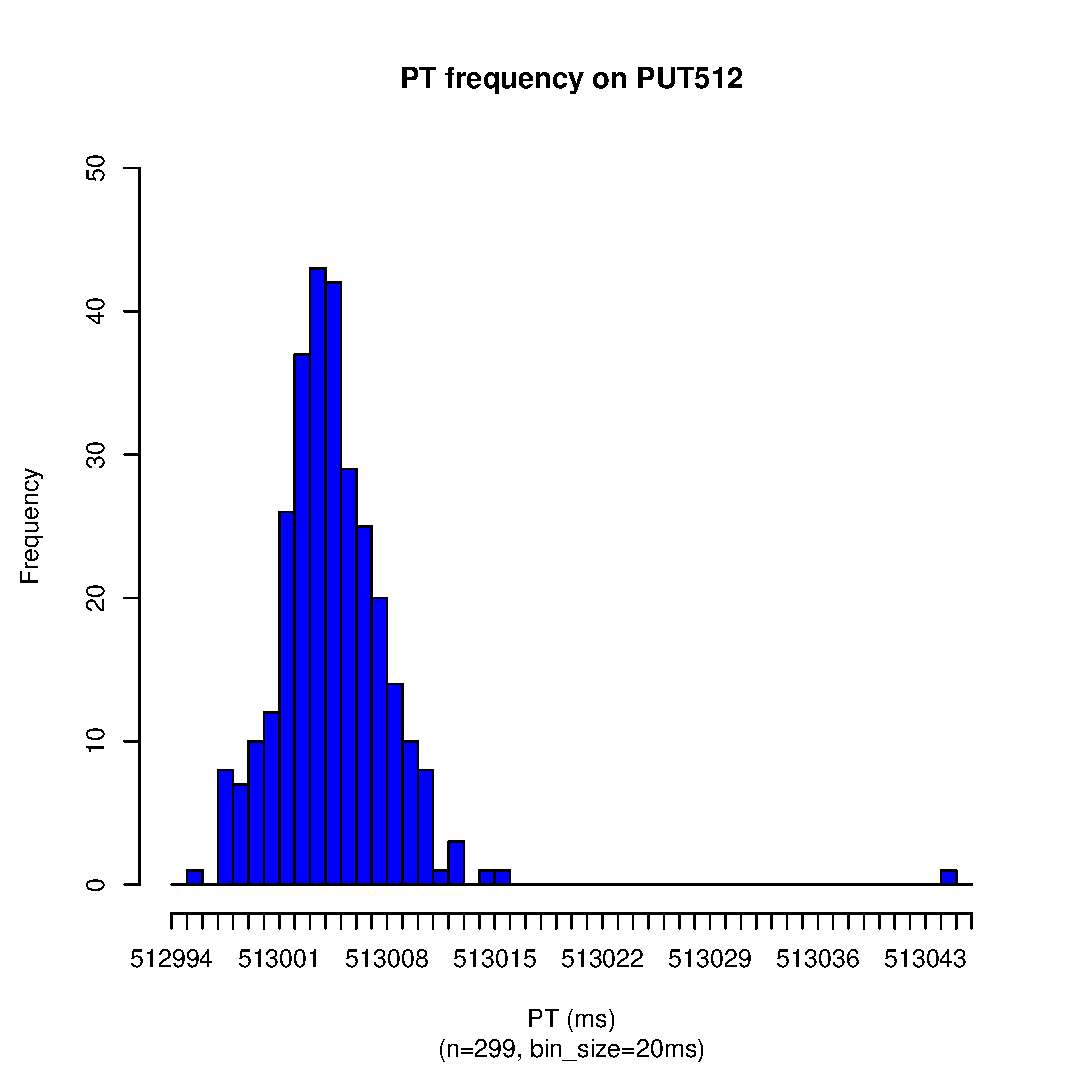
\includegraphics[scale=0.43]{512_sec_pt_hist2.eps}
		\label{fig:put512_hist2}
	}
	\subfigure[PT frequency on PUT1024]{
		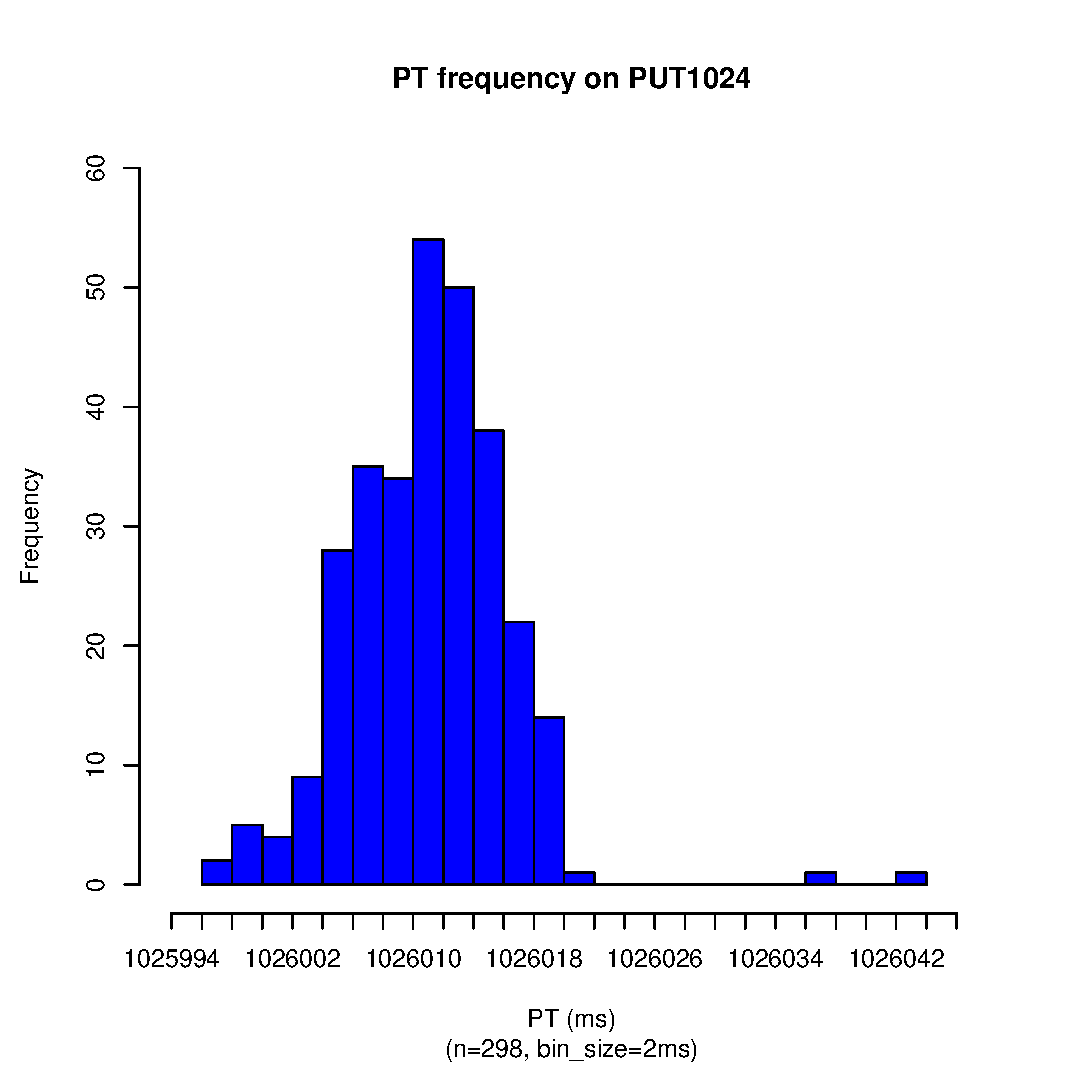
\includegraphics[scale=0.43]{1024_sec_pt_hist2.eps}
		\label{fig:put1024_hist2}
	}
	\caption{PT Histograms of PUT128 ... PUT1024~\label{fig:pt_out_hist3}}
\end{figure}

\newpage

\begin{figure}[hp!]
	\centering
	\subfigure[PT frequency on PUT2048]{
		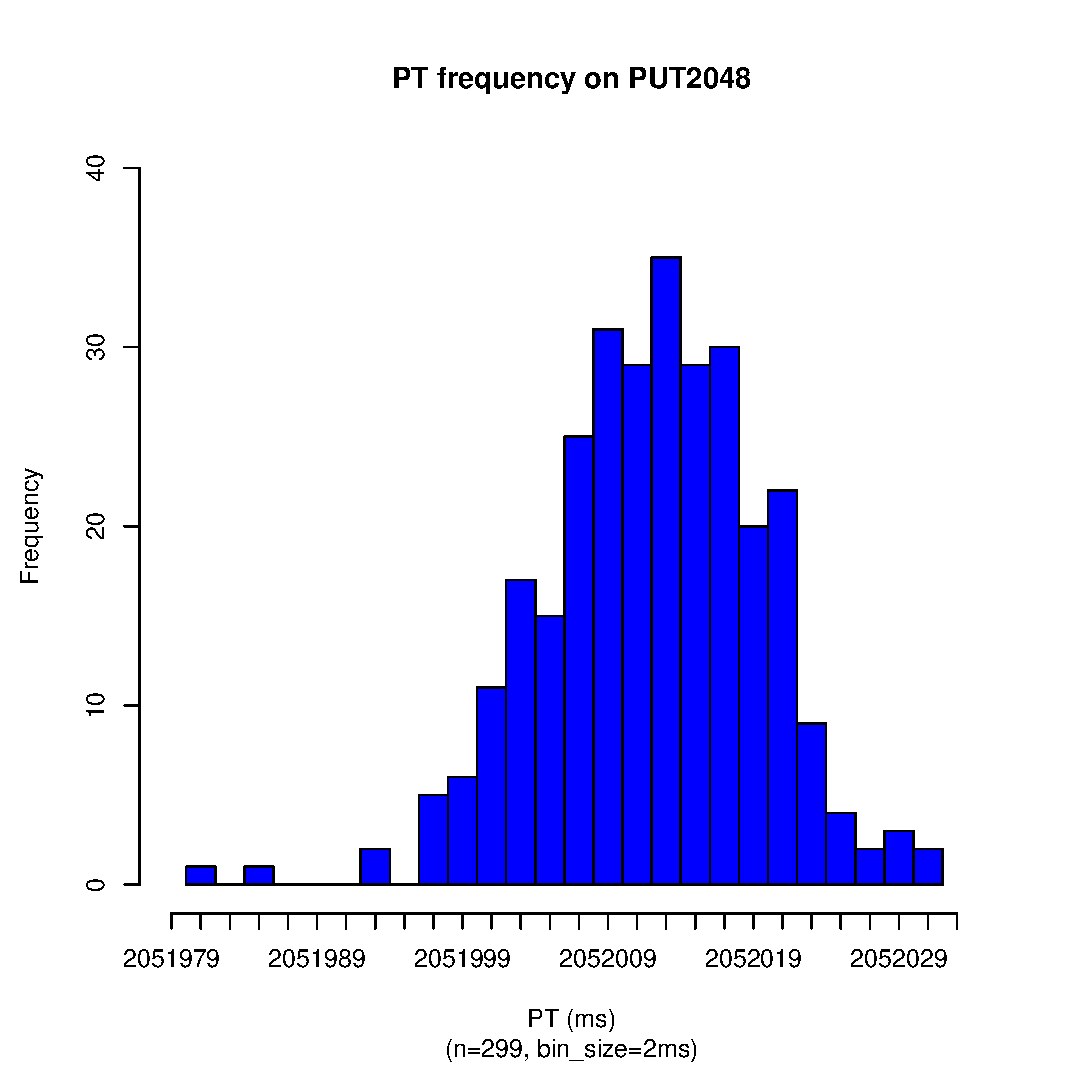
\includegraphics[scale=0.43]{2048_sec_pt_hist2.eps}
		\label{fig:put2048_hist2}
	}
	\subfigure[PT frequency on PUT4096]{
		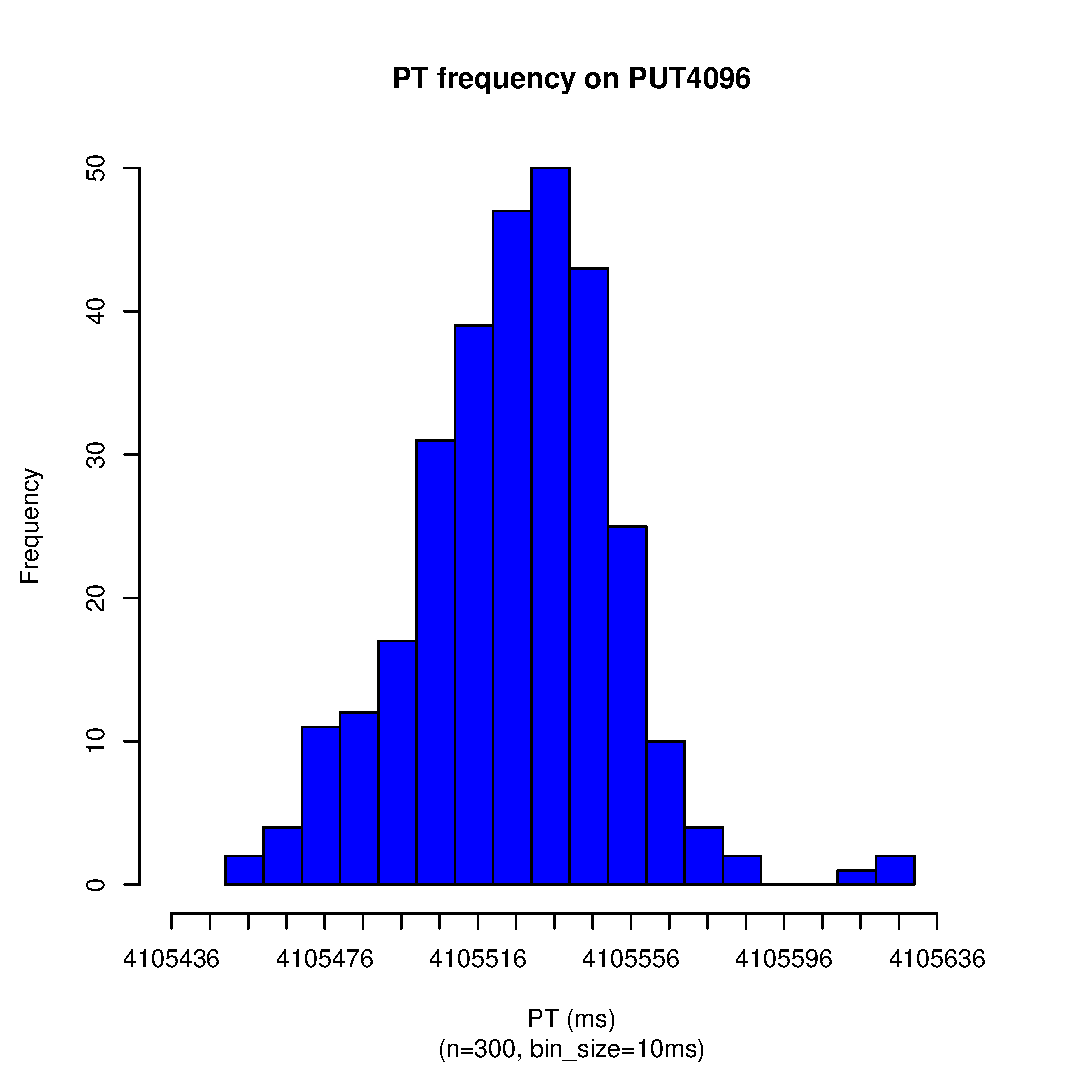
\includegraphics[scale=0.43]{4096_sec_pt_hist2.eps}
		\label{fig:put4096_hist2}
	}
	\caption{PT Histograms of PUT2048 and PUT4096~\label{fig:pt_out_hist4}}
\end{figure}

\newpage

\begin{figure}[hp!]
	\centering
	\subfigure[PT frequency on PUT8192 with 40 samples (See Table~\ref{tab:exp_notes1}.)]{
		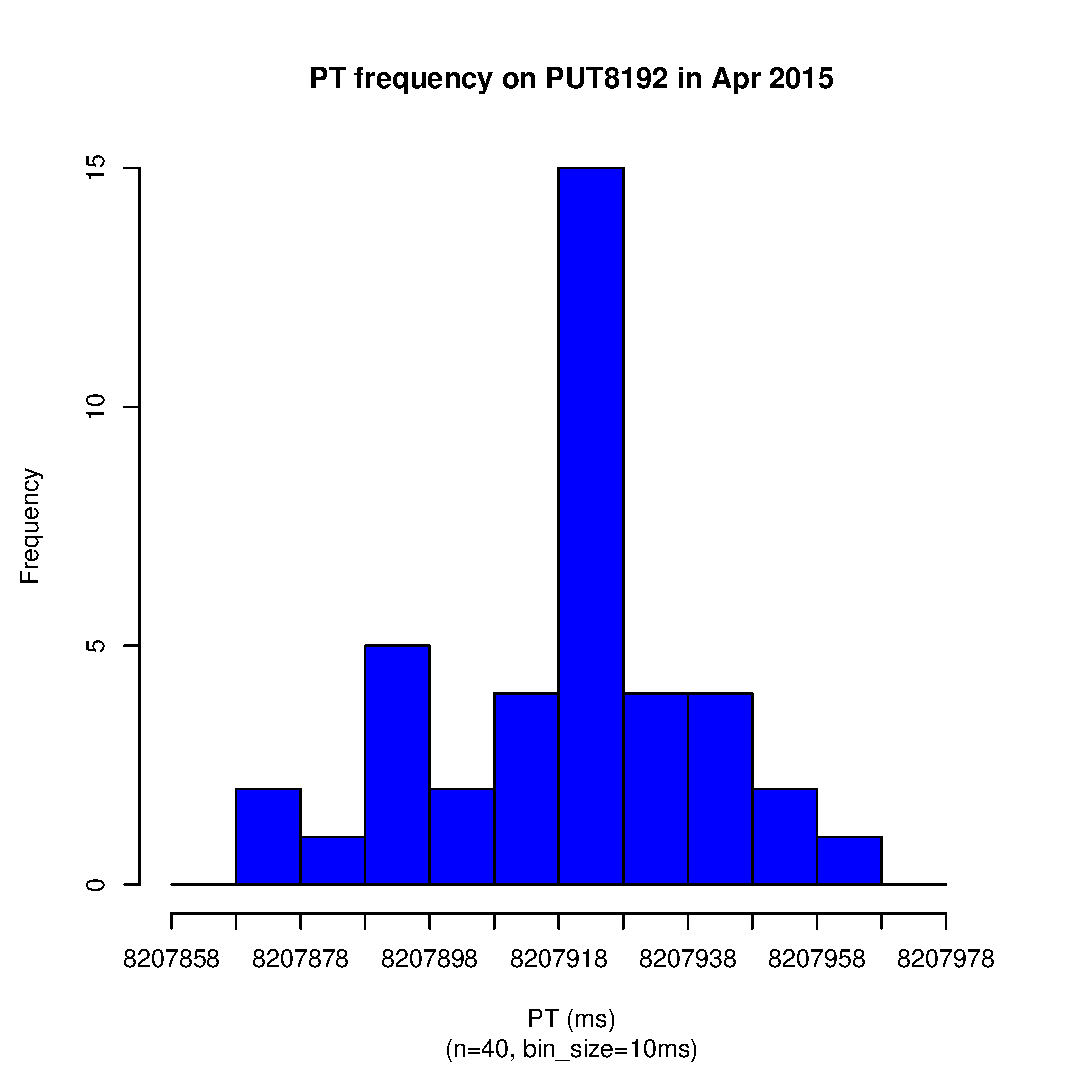
\includegraphics[scale=0.43]{8192_sec_pt_hist_out1.eps}
		\label{fig:put8192_out_hist1}
	}
	\subfigure[PT frequency on PUT8192 with 260 samples (See Table~\ref{tab:exp_notes1}.)]{
		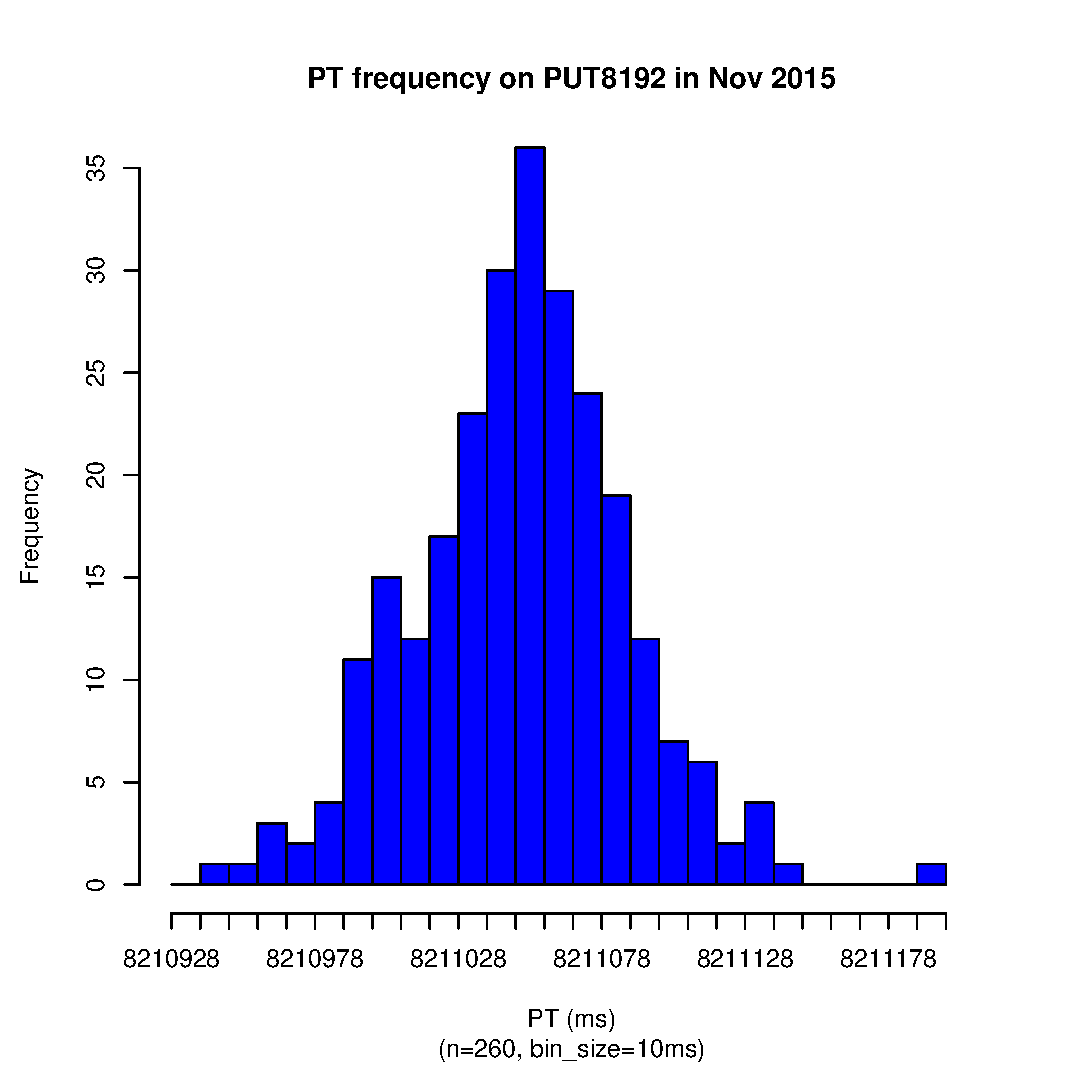
\includegraphics[scale=0.43]{8192_sec_pt_hist_out2.eps}
		\label{fig:put8192_out_hist2}
	}
	\subfigure[PT frequency on PUT16384 with 40 samples (See Table~\ref{tab:exp_notes1}.)]{
		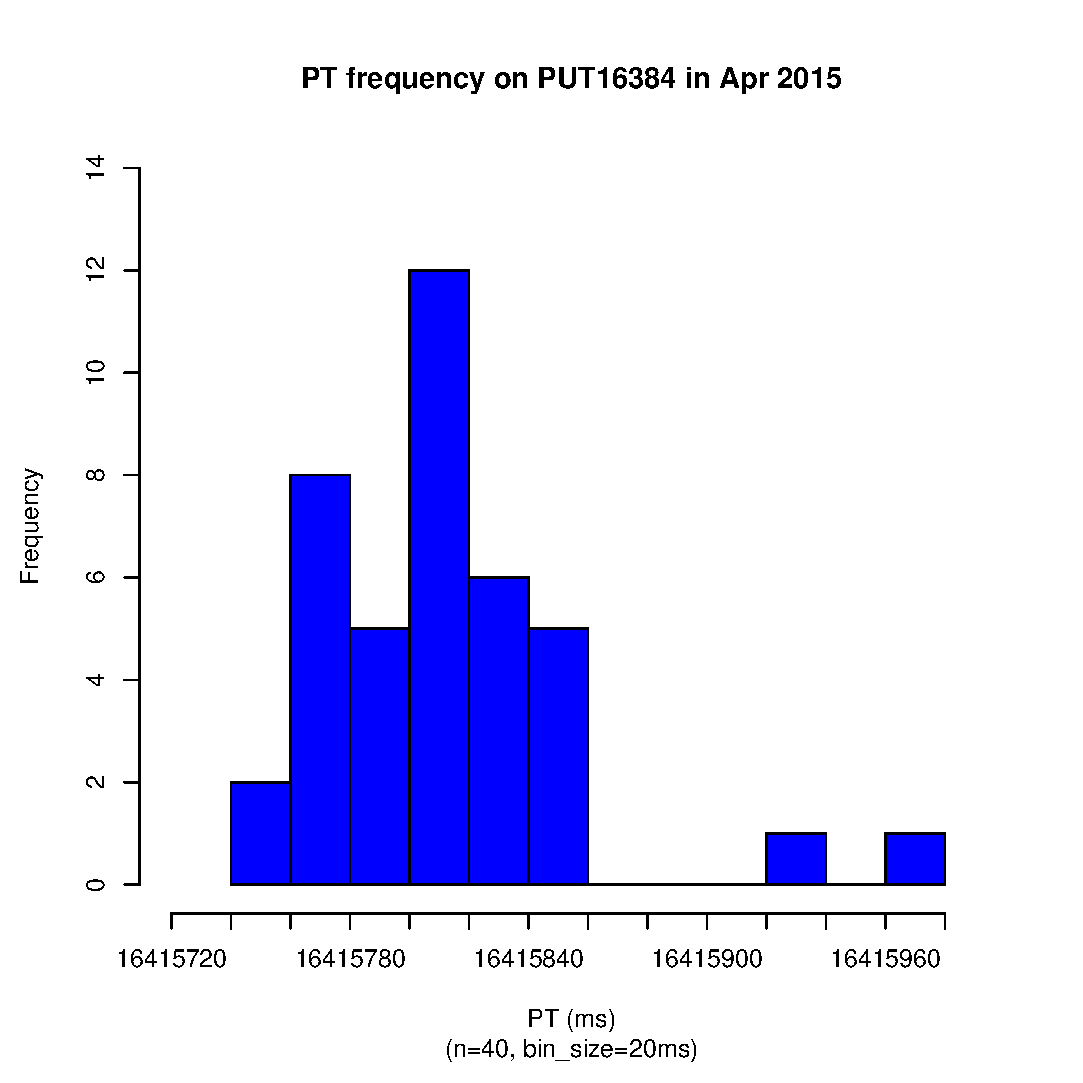
\includegraphics[scale=0.43]{16384_sec_pt_hist_out1.eps}
		\label{fig:put16384_out_hist1}
	}
	\subfigure[PT frequency on PUT16384 with 260 samples (See Table~\ref{tab:exp_notes1}.))]{
		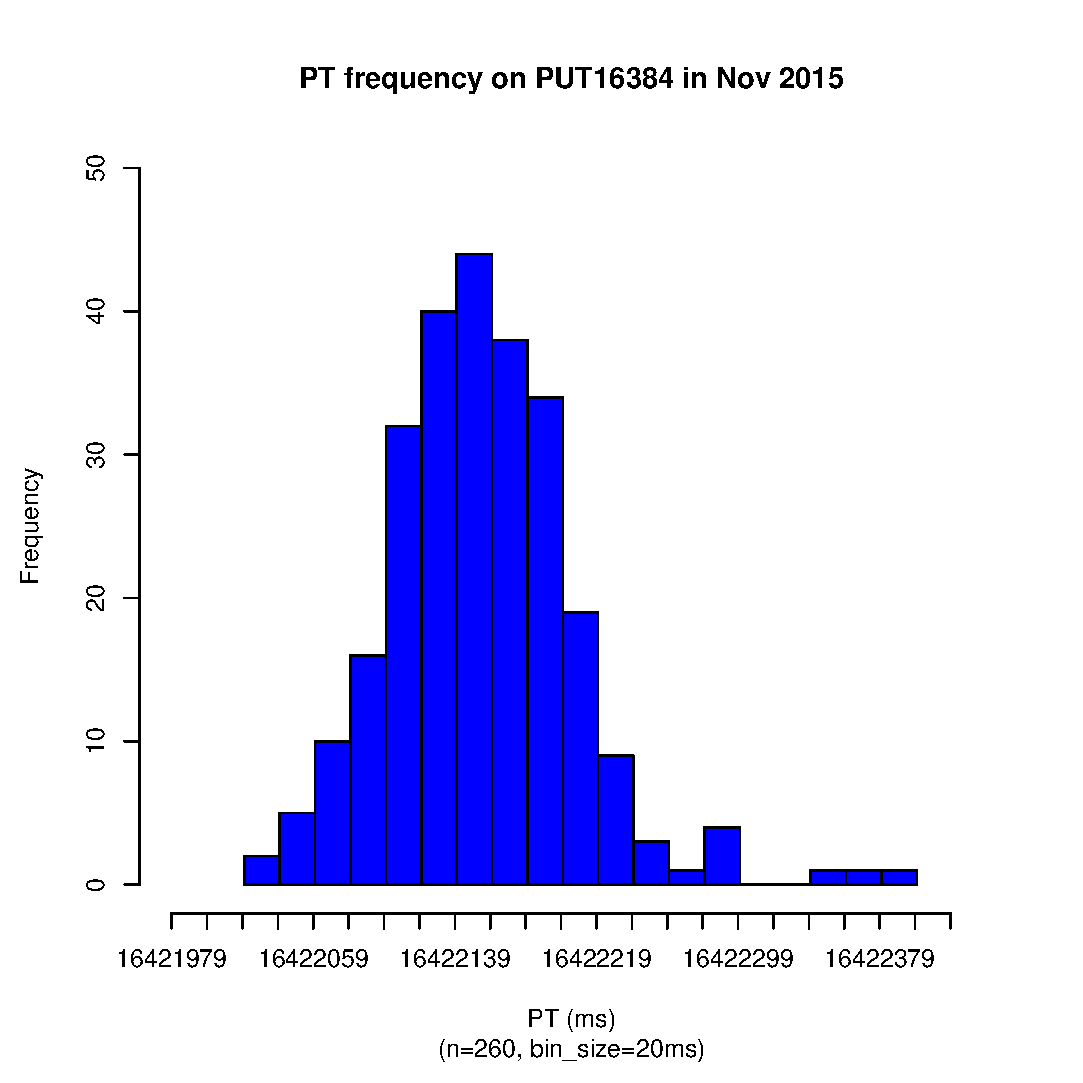
\includegraphics[scale=0.43]{16384_sec_pt_hist_out2.eps}
		\label{fig:put16384_out_hist2}
	}
	\caption{PT Histograms of PUT8192 and PUT16384~\label{fig:pt_out_hist5}}
\end{figure}

%%% section 5
\clearpage
\newpage

\section{Sample Size vs. Standard Deviation of PT~\label{sec:new_put}}
The base data of the following histograms are from Table~\ref{tab:exp_notes3}.

\subsection{PUT1 and PUT2~\label{sec:put1_put2}}
Table~\ref{fig:put_std} exhibits varying standard deviations 
over increasing sample size on PUT1 and PUT2.
EMPv4 is applied to the table's data.

\begin{table}[h]
\centering
{
 \begin{tabular}{|l|c|c|} \hline
\multirow{2}{*}{Num. of Samples}   & \multicolumn{2}{|c|}{Std. Dev. (msec)} \\  \cline{2-3}
						    & PUT1 & PUT2 \\  \hline\hline
1,000 & 1.07 & 1.40\\ \hline
2,000 & 1.06 & 1.39\\ \hline
3,000 & 1.07 & 1.38\\ \hline
4,000 & 1.07 & 1.37\\ \hline
5,000 & 1.07 & 1.40\\ \hline
6,000 & 1.06& 1.70\\ \hline
7,000 & 1.06& 1.65\\ \hline
8,000 & 1.07&1.62\\ \hline
9,000 & 1.07&1.60\\ \hline
10,000 & 1.07&1.58\\ \hline
11,000 & 1.08&1.57\\ \hline
12,000 & 1.08&1.56\\ \hline
13,000 & 1.08&1.54\\ \hline
14,000 & 1.08&1.53\\ \hline
15,000 & 1.08&1.52\\ \hline
16,000 & 1.08&1.51\\ \hline
17,000 & 1.08&1.50\\ \hline
18,000 & 1.08&1.50\\ \hline
19,000 & 1.08&1.50\\ \hline 
20,000 & 1.08& 1.49\\ \hline 
  \end{tabular}
  }
 \caption{Std. Dev. of PUT1 and PUT2 over increasing sample size~\label{fig:put_std}}
\end{table}
 
 \newpage
 
\begin{figure}[hp!]
	\centering
	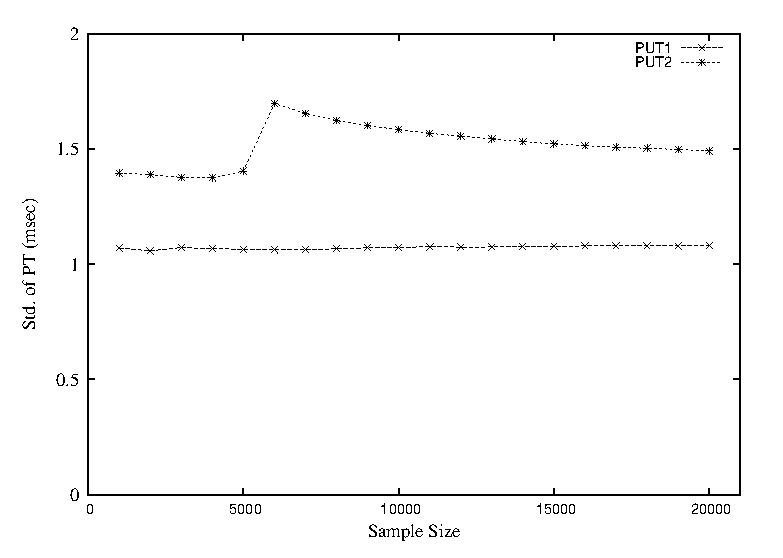
\includegraphics[scale=0.8]{put_pt_std.eps}
	\caption{Std. dev. of PT on PUT1 and PUT2 over increasing sample size ~\label{fig:std_ss}}
\end{figure}

\begin{figure}[hp!]
	\centering
	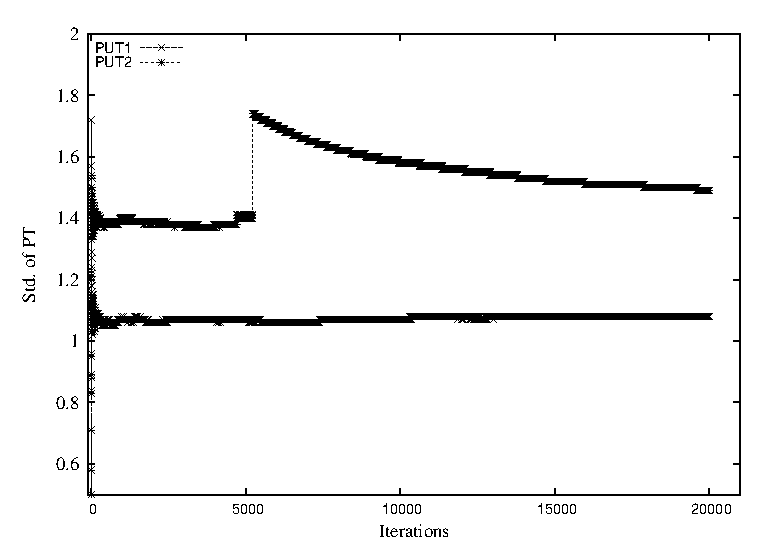
\includegraphics[scale=0.8]{put_pt_20k_std.eps}
	\caption{Std. dev. of PT on PUT1 and PUT2 over increasing sample size ~\label{fig:detailed_std_ss}}
\end{figure}

\begin{table}
\centering
{
 \begin{tabular}{|l|l|} \hline
PUT2  & Program Time \\ \hline
{\tt incr\_work} & 2078 msecs (at the 5276th iteration)\\ \hline \hline
Daemon Processes  & Program Time \\ \hline
{\tt md0\_raid1} & 1 msec\\ \hline
{\tt proc\_monitor} & 198 msecs\\ \hline
{\tt rhn\_check} & 460 msecs\\ \hline \hline
{\bf Total} & 659 msecs\\ \hline
  \end{tabular}
  }
 \caption{The daemon processes captured at the hike of PUT2~\label{fig:daemon}}
\end{table}

\begin{figure}
	\centering
	\subfigure[PT frequency on PUT1 by EMPv4 (See Table~\ref{tab:exp_notes3}.)]{
		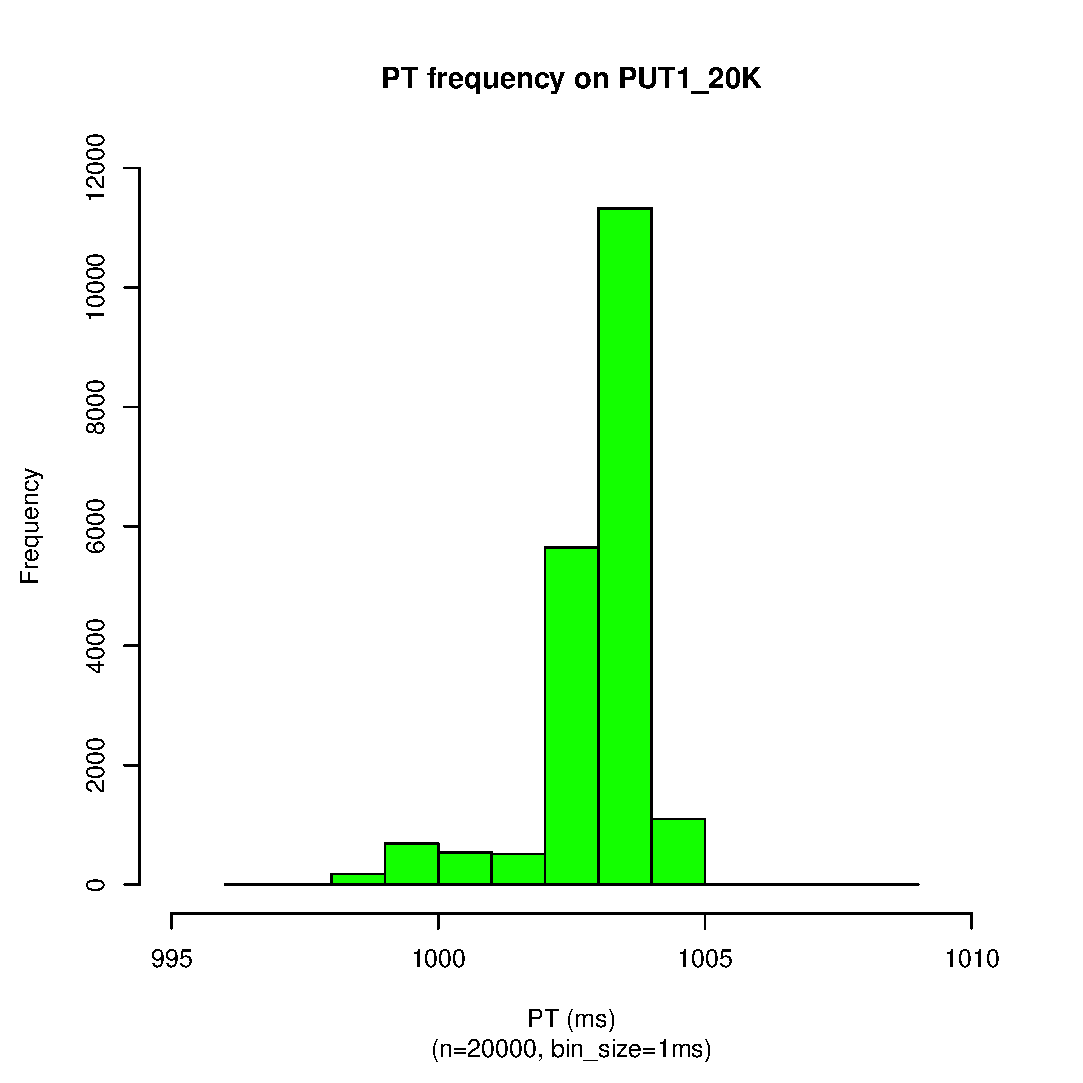
\includegraphics[scale=0.43]{put1_20k_hist.eps}
		\label{fig:put1_20k_hist1}
	}
	\subfigure[PT frequency on PUT1 by EMPv5 (See Table~\ref{tab:exp_notes3}.)]{
		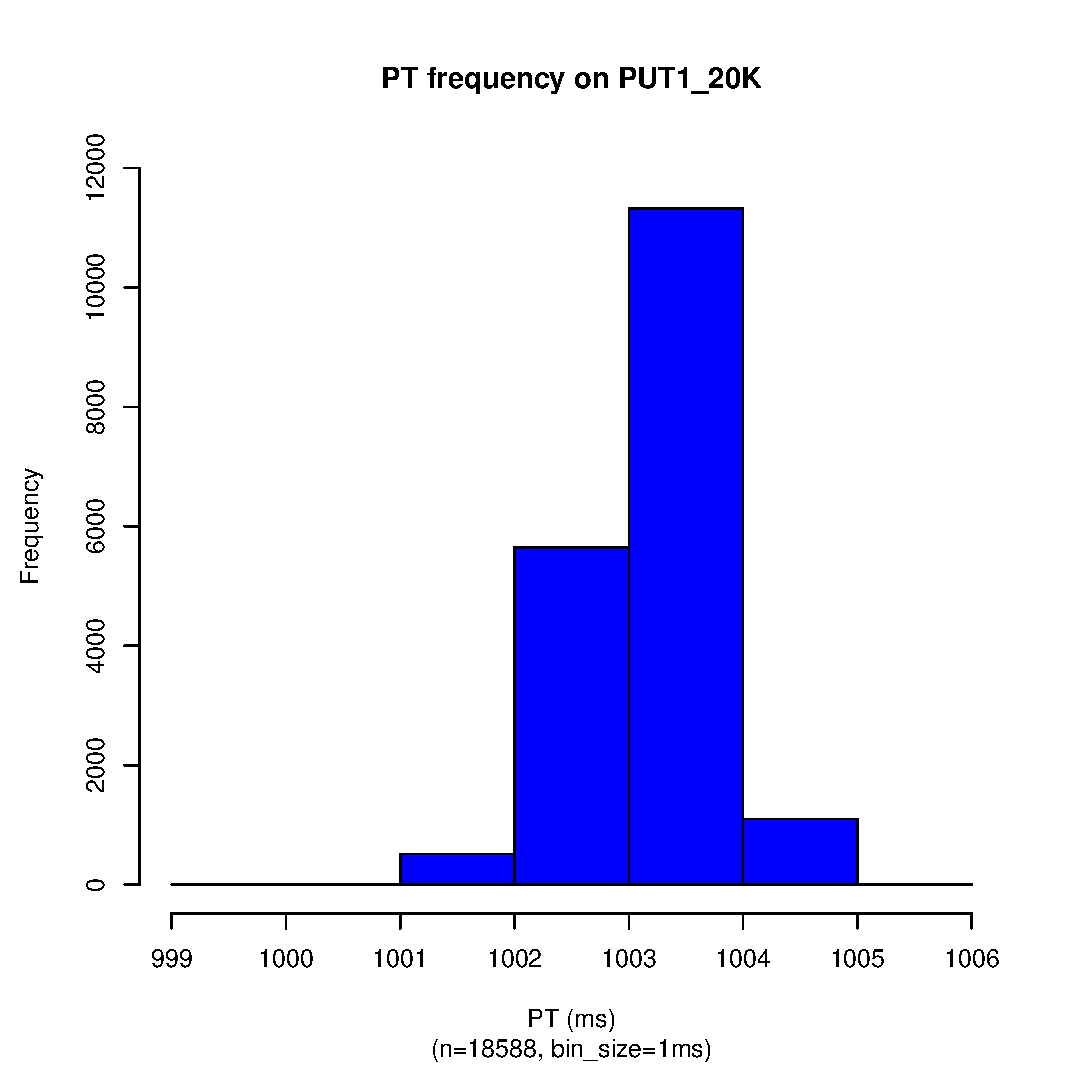
\includegraphics[scale=0.43]{put1_20k_hist2.eps}
		\label{fig:put1_20k_hist2}
	}
	\subfigure[PT frequency on PUT2 by EMPv4  (See Table~\ref{tab:exp_notes3}.)]{
		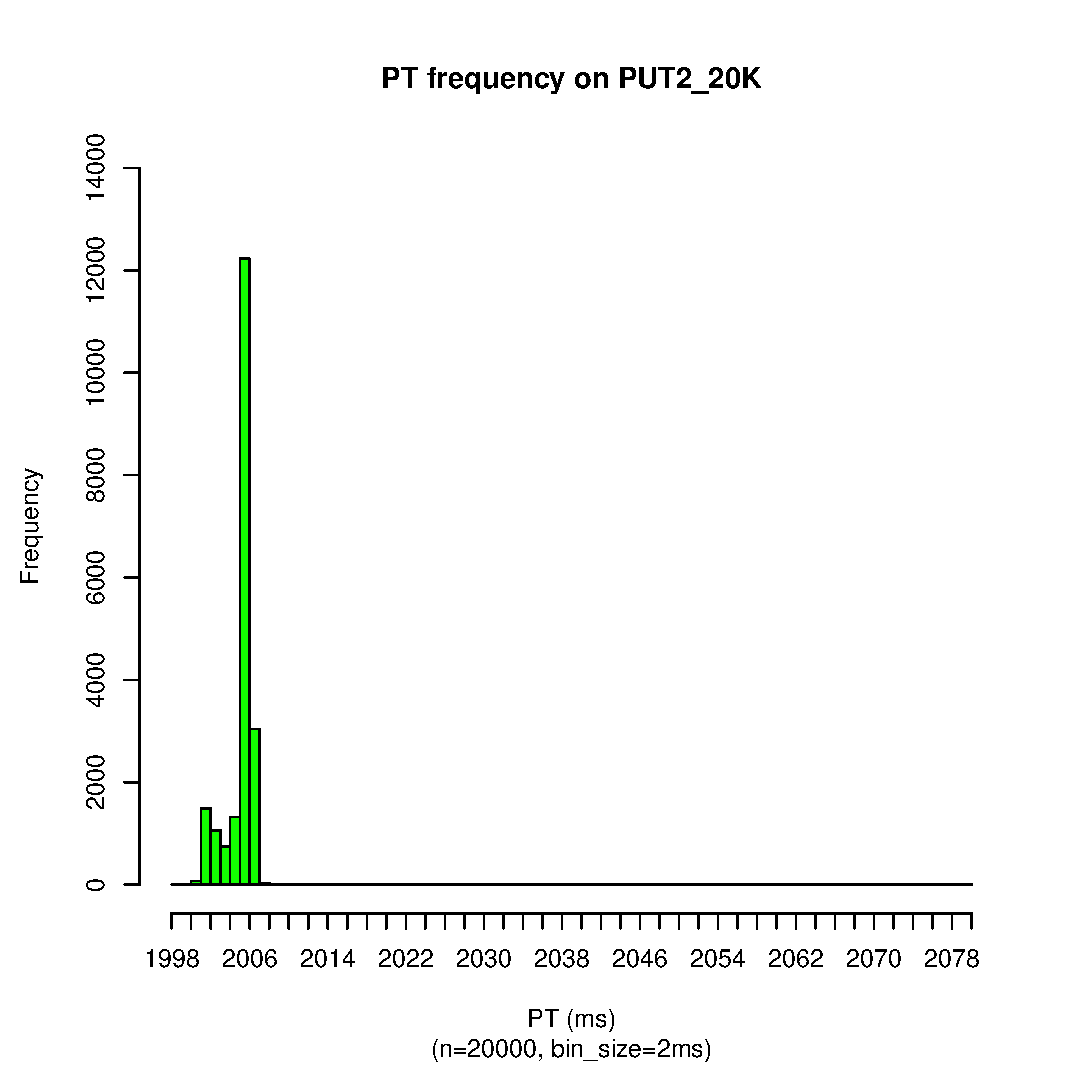
\includegraphics[scale=0.43]{put2_20k_hist.eps}
		\label{fig:put2_20k_hist3}
	}
	\subfigure[PT frequency on PUT2 by EMPv5 (See Table~\ref{tab:exp_notes3}.)]{
		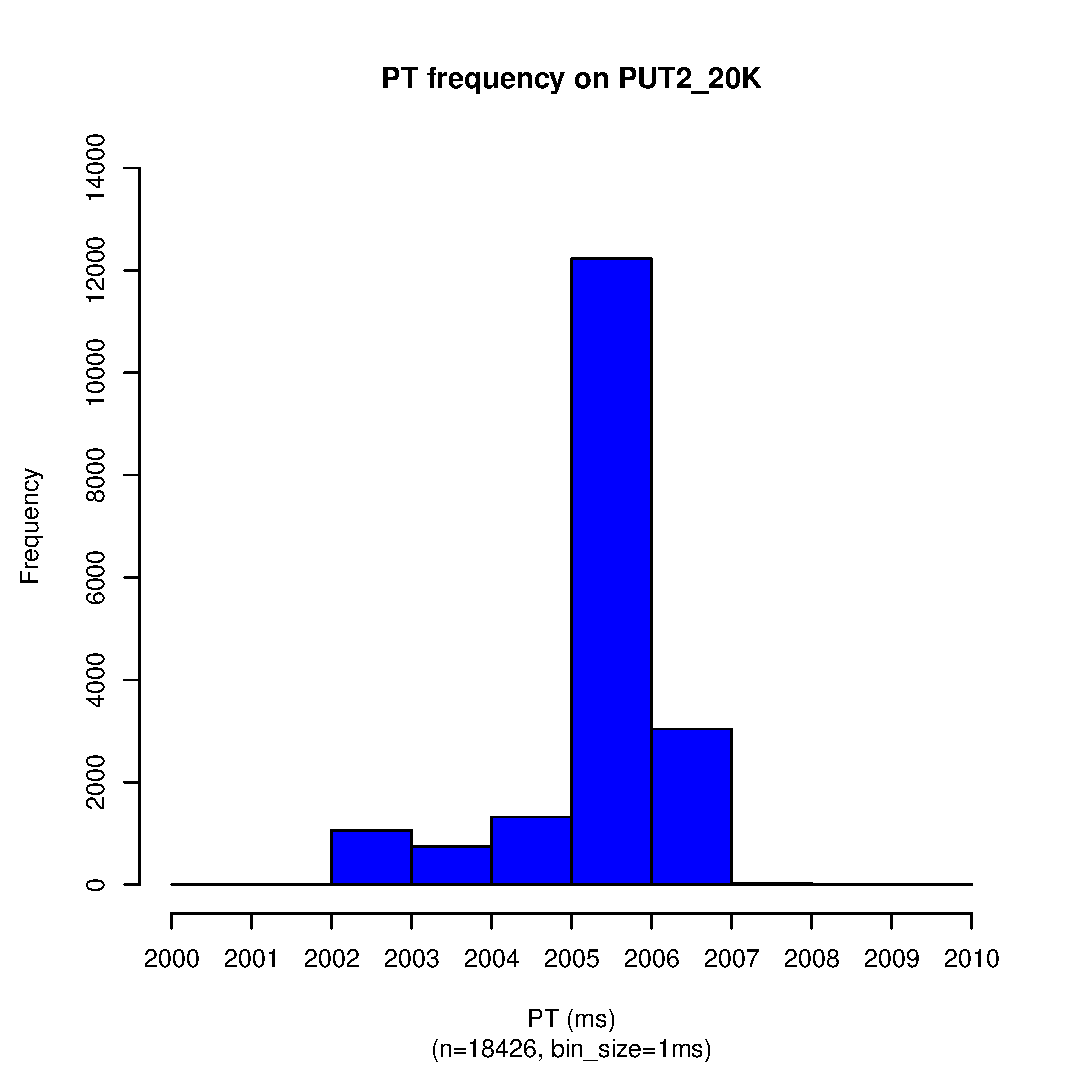
\includegraphics[scale=0.43]{put2_20k_hist2.eps}
		\label{fig:put2_20k_hist4}
	}
	\caption{PT Histograms of PUT1 and PUT2 by 20,000 trials~\label{fig:put_x_20k}}
\end{figure}

\begin{figure}
	\centering
	\subfigure[PT frequency on PUT4 by EMPv4 (See Table~\ref{tab:exp_notes3}.)]{
		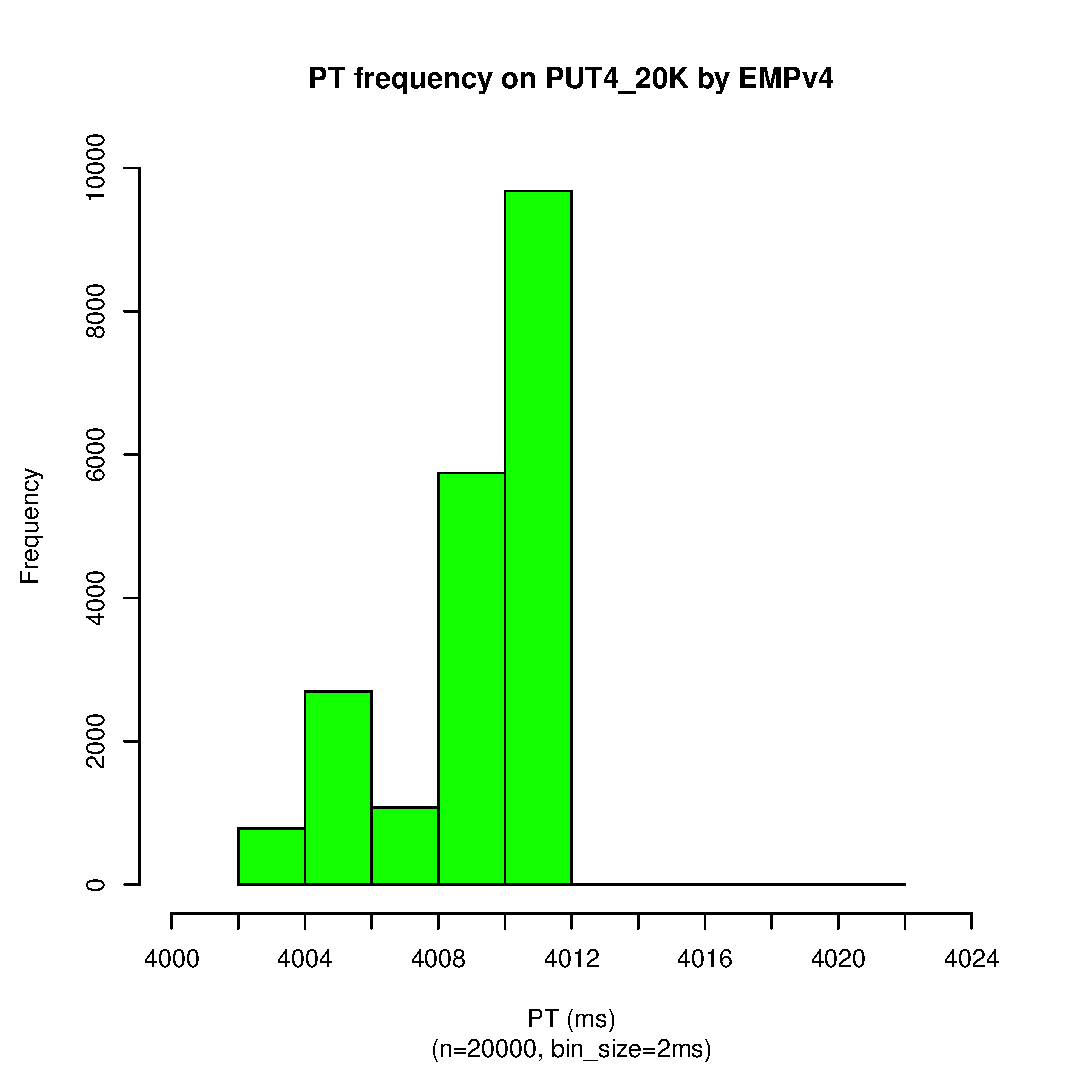
\includegraphics[scale=0.43]{put4_20k_hist.eps}
		\label{fig:put4_20k_hist1}
	}
	\subfigure[PT frequency on PUT4 by EMPv5 (See Table~\ref{tab:exp_notes3}.)]{
		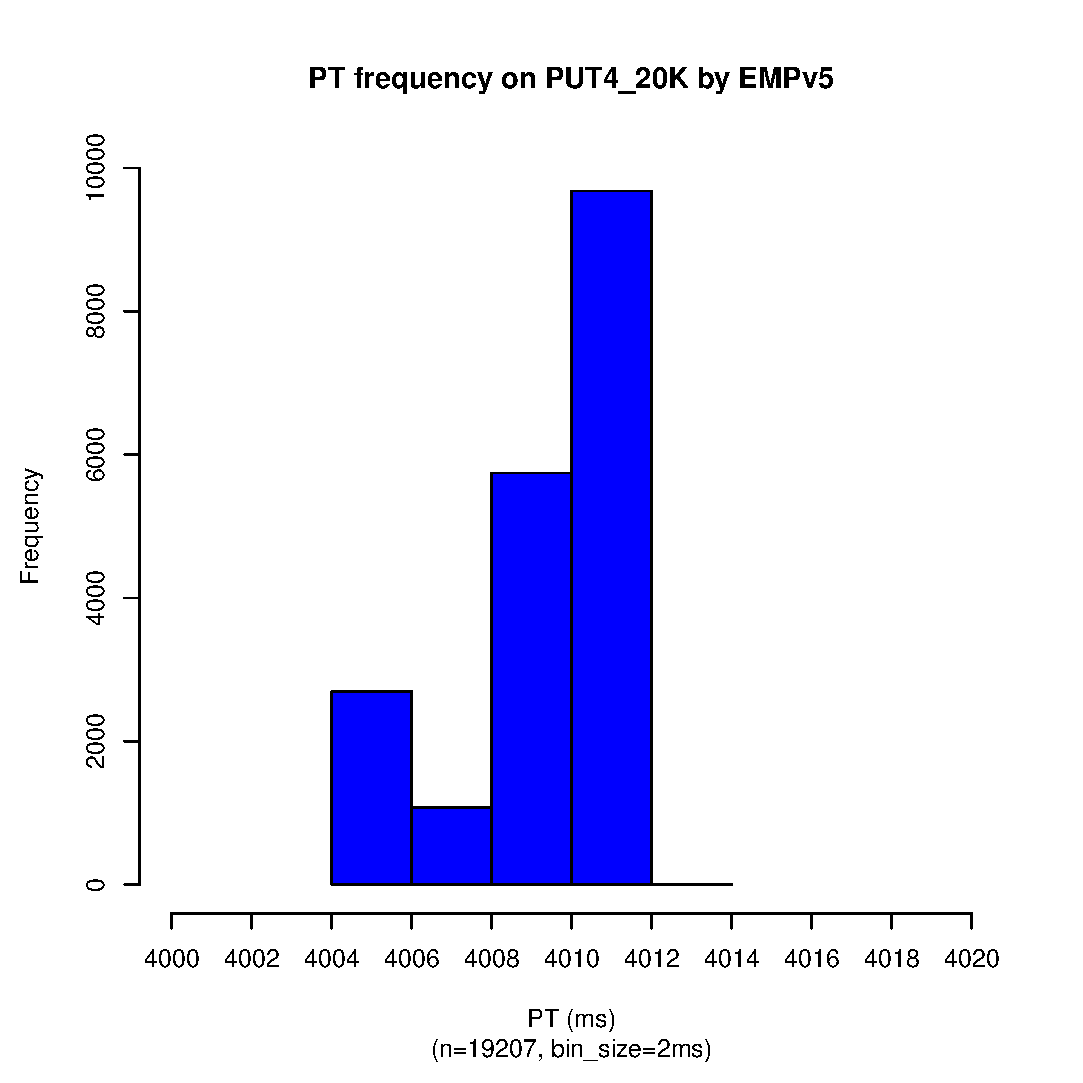
\includegraphics[scale=0.43]{put4_20k_hist2.eps}
		\label{fig:put4_20k_hist2}
	}
	\subfigure[PT frequency on PUT8 by EMPv4  (See Table~\ref{tab:exp_notes3}.)]{
		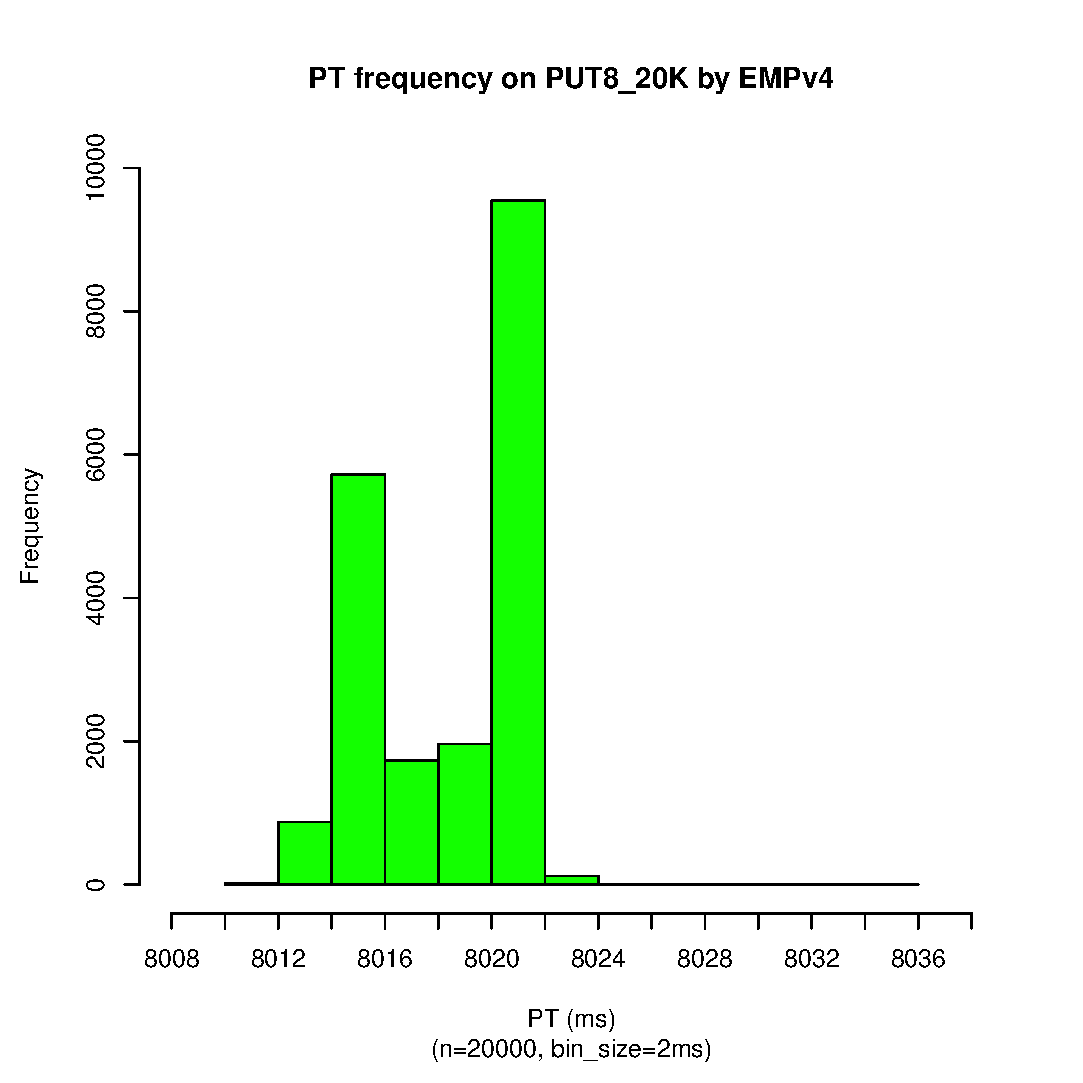
\includegraphics[scale=0.43]{put8_20k_hist.eps}
		\label{fig:put8_20k_hist3}
	}
	\subfigure[PT frequency on PUT8 by EMPv5 (See Table~\ref{tab:exp_notes3}.)]{
		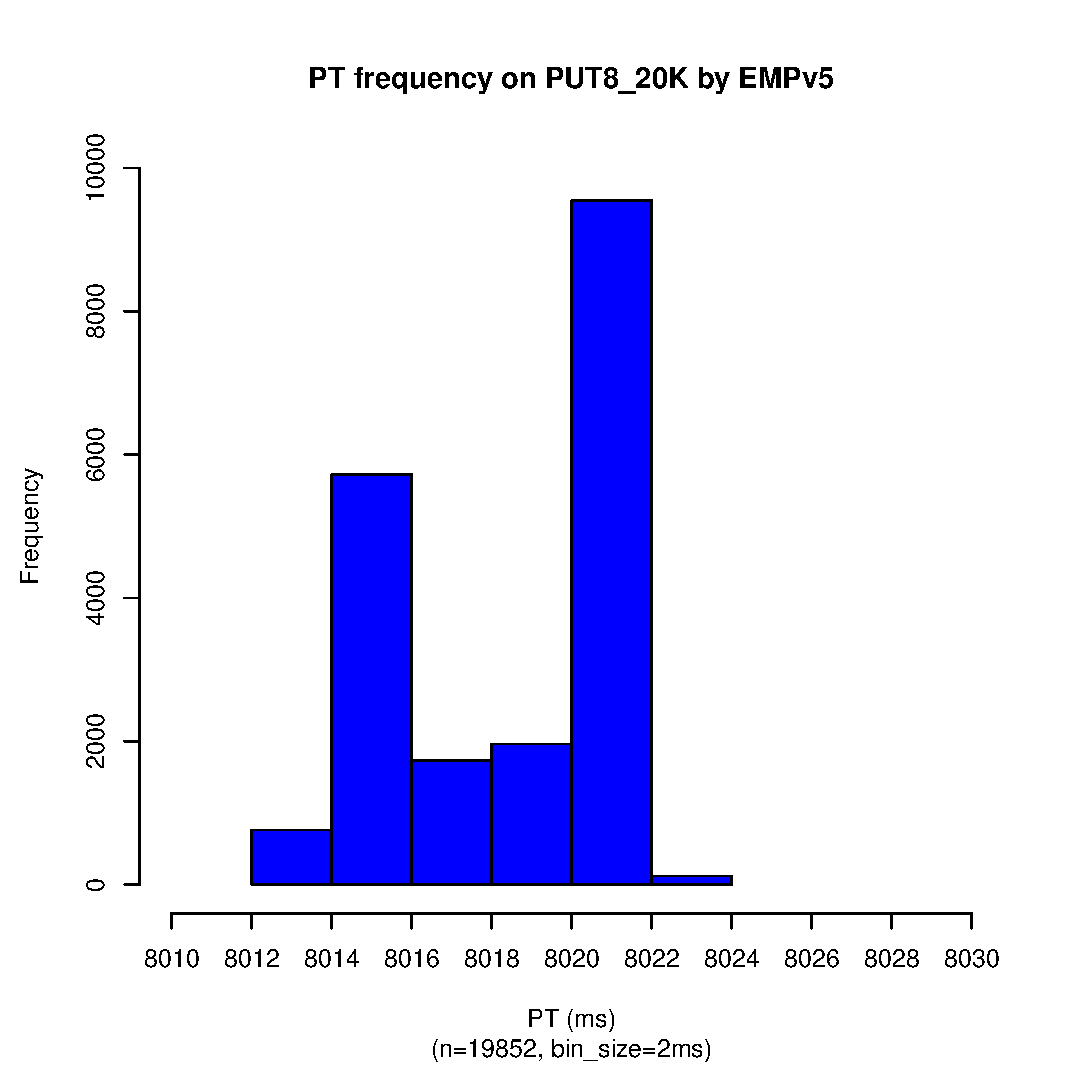
\includegraphics[scale=0.43]{put8_20k_hist2.eps}
		\label{fig:put8_20k_hist4}
	}
	\caption{PT Histograms of PUT4 and PUT8 by 20,000 trials~\label{fig:put_x_20k_2}}
\end{figure}

\newpage

\subsection{PUT16~\label{sec:put16_ss}}
In this experiment we ran PUT16 up to 32,000 from 1,000 times by a factor of two.
The relaxed version of EMPv5 (called {\em EMPv5-relaxed}) uses *five* standard deviations 
whereas its strict version (called {\em EMPv5-strict})  does *two* standard deviations for a vertical gap below and above the average.
(Young: 2k samples seem most appropriate to represent the whole population of PUT16, 
in that the standard deviations by EMPv5 on the 2k sample size are almost at peak compared 
to those of the other sample sizes.)

\begin{table}[h]
\centering
{
 \begin{tabular}{|l|c|c|c|} \hline
\multirow{2}{*}{Num. of Samples}   & \multicolumn{3}{|c|}{Std. Dev. (msec)} \\  \cline{2-4}
						    & EMPv4 & EMPv5-relaxed & EMPv5-strict \\  \hline
1,000 & 1.86 & 1.86  & 1.68\\ \hline
2,000 & 2.20 & 2.12 & 1.81\\ \hline
4,000 & 2.21 & 1.89 & 1.65\\ \hline
8,000 & 2.23 & 1.97 & 1.71\\ \hline
16,000 & 2.07 & 2.00 & 1.61\\ \hline
32,000 & 1.81 & 1.75 & 1.53\\ \hline
  \end{tabular}
  }
 \caption{Standard deviations of PUT16 over increasing sample size~\label{fig:put16_std_ss_summary}}
\end{table}

%\begin{figure}[hp!]
%	\centering
%	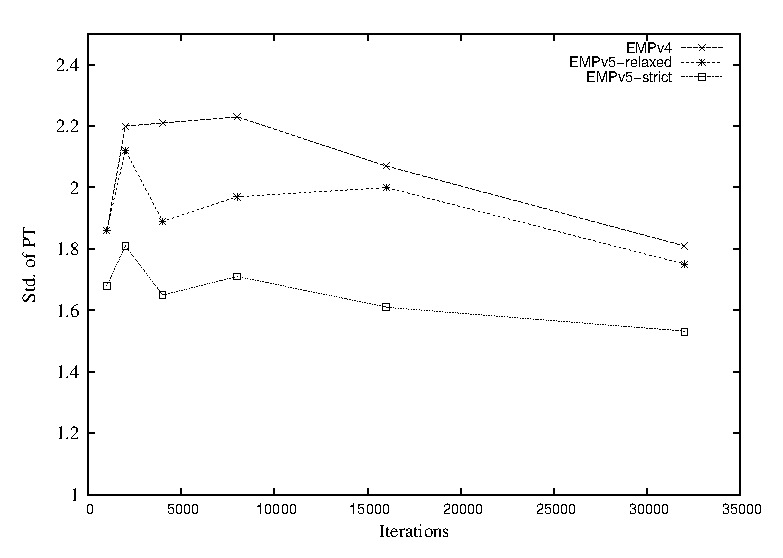
\includegraphics[scale=0.8]{put16_std_ss.eps}
%	\caption{Std. dev. of PT on PUT16 over increasing sample size ~\label{fig:put16_std_ss_plot}}
%\end{figure}

\begin{figure}[h]
	\centering
	\subfigure[Standard deviations of PT on PUT16]{
		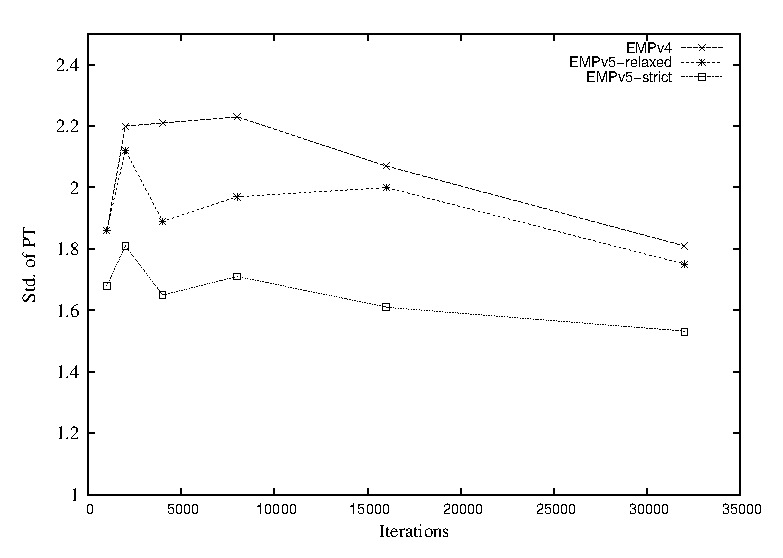
\includegraphics[scale=0.62]{put16_std_ss.eps}
		\label{fig:put16_std}
	}
	\subfigure[Standard deviations of PT on PUT16, in log scale]{
		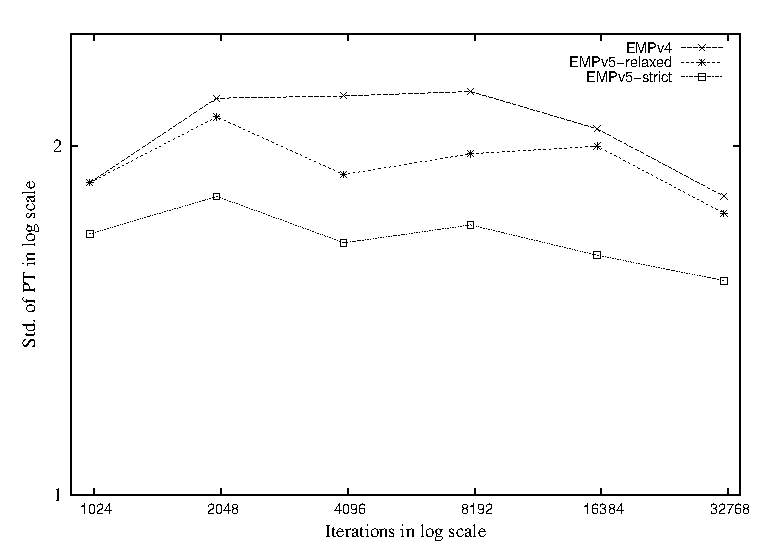
\includegraphics[scale=0.62]{put16_std_ss_log.eps}
		\label{fig:put16_std_log}
	}
	\caption{Standard deviations of PT on PUT16 over increasing sample size~\label{fig:put16_std_ss_plot}}
\end{figure}

\clearpage
\newpage

\subsection{Histograms by EMPv4~\label{sec:put16_empv4}}
We apply EMPv4 to the runs of PUT16 as mentioned above.
The following histograms are the results of EMPv4.

\begin{figure}[hp!]
	\centering
	\subfigure[PT frequency on PUT16 with 1k samples]{
		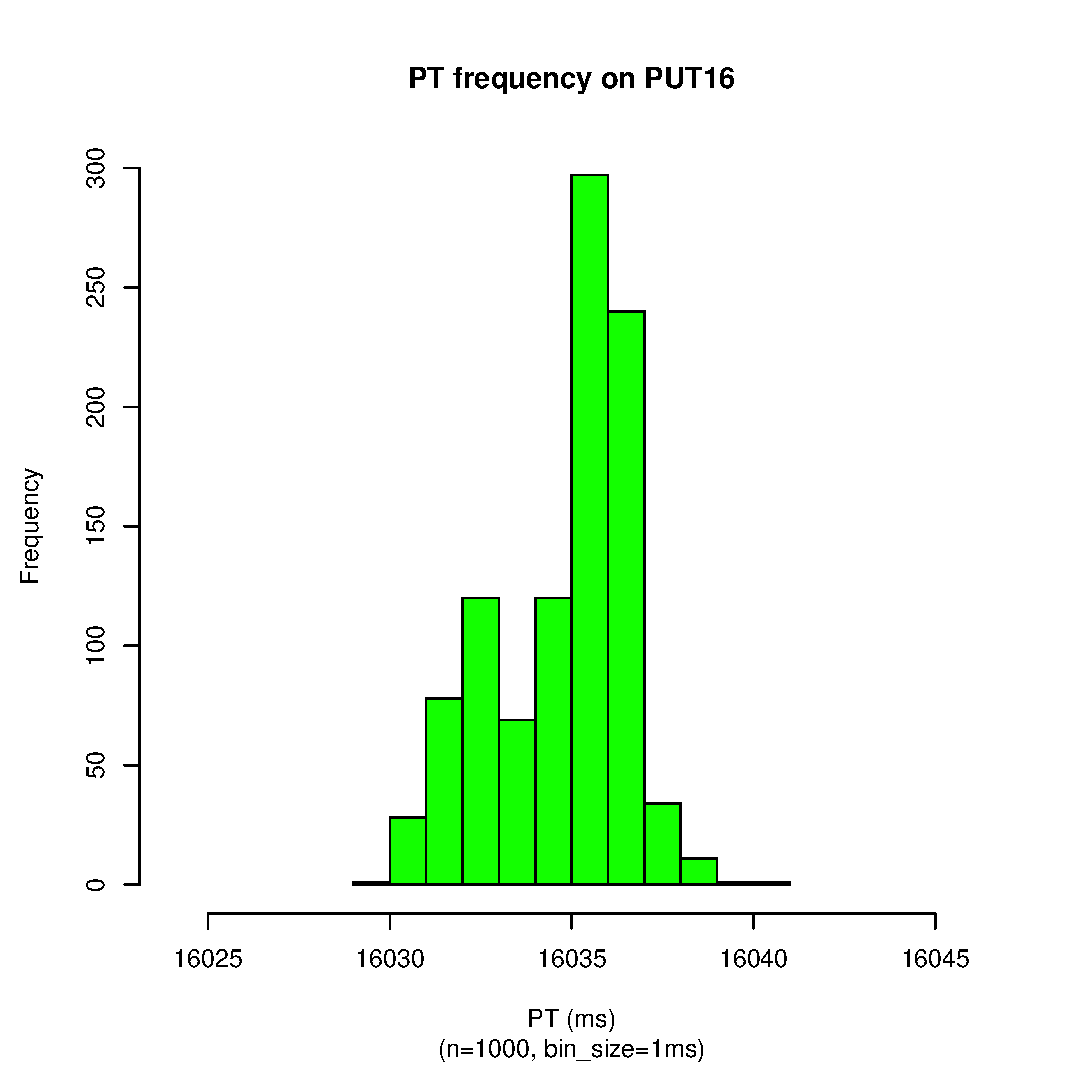
\includegraphics[scale=0.43]{16_sec_pt_hist.eps}
		\label{fig:put16_1k_hist}
	}
	\subfigure[PT frequency on PUT16 with 2k samples]{
		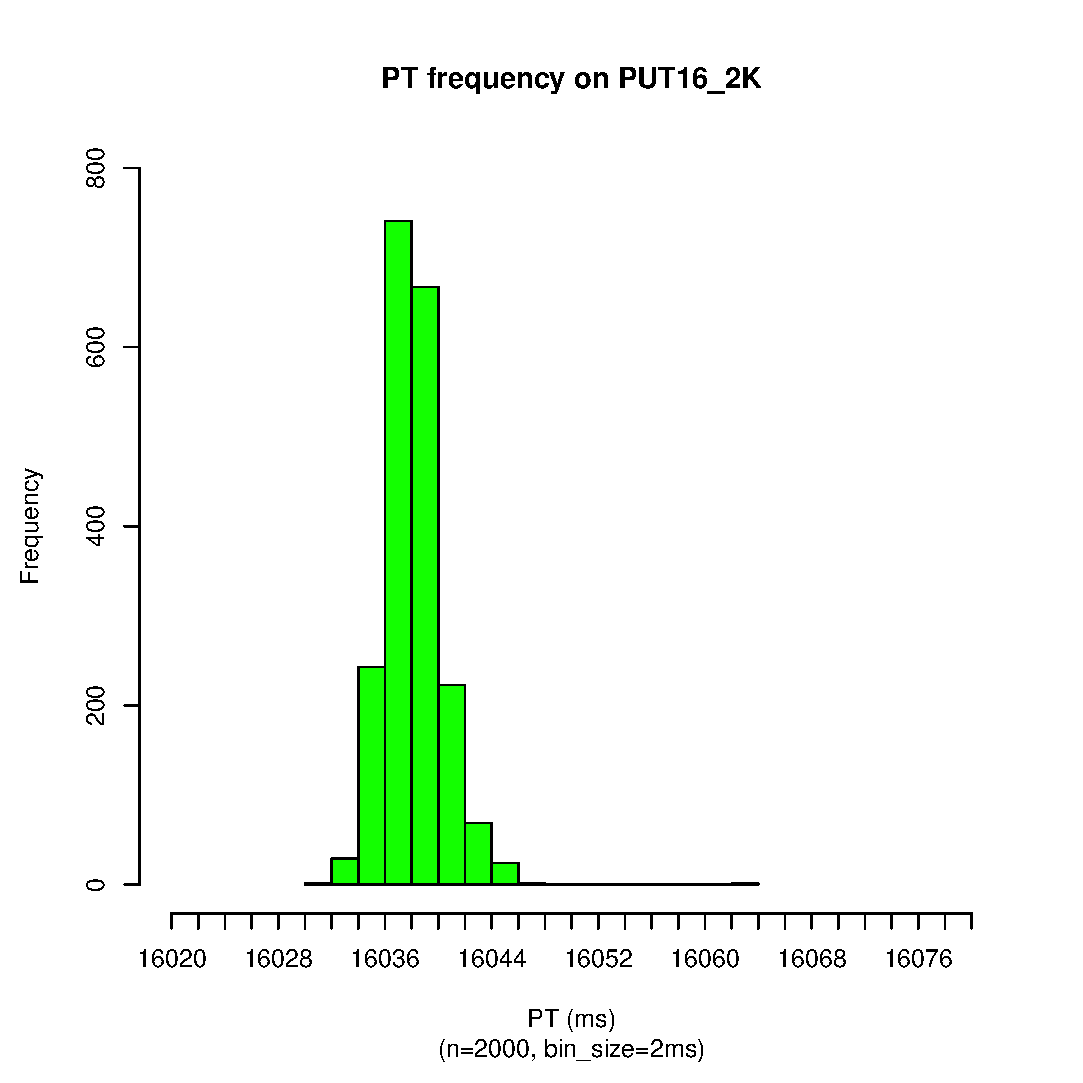
\includegraphics[scale=0.43]{16_sec_2k_hist.eps}
		\label{fig:put16_2k_hist}
	}
	\subfigure[PT frequency on PUT16 with 4k samples]{
		\includegraphics[scale=0.43]{16_sec_4k_hist.eps}
		\label{fig:put16_4k_hist}
	}
	\subfigure[PT frequency on PUT16 with 8k samples]{
		\includegraphics[scale=0.43]{16_sec_8k_hist.eps}
		\label{fig:put16_8k_hist}
	}
	\caption{PT histogram of PUT16 by EMPv4, with the sample size increasing from 1k to 8k~\label{fig:put16_ss1_empv4}}
\end{figure}

\begin{figure}[H]
	\centering
	\subfigure[PT frequency on PUT16 with 16k samples]{
		\includegraphics[scale=0.43]{16_sec_16k_hist.eps}
		\label{fig:put16_16k_hist}
	}
	\subfigure[PT frequency on PUT16 with 32k samples]{
		\includegraphics[scale=0.43]{16_sec_32k_hist.eps}
		\label{fig:put16_32k_hist}
	}
	\caption{PT histogram of PUT16 by EMPv4, with the sample size increasing from 16k to 32k~\label{fig:put16_ss2_empv4}}
\end{figure}

\clearpage
\newpage

\subsection{Histograms by EMPv5~\label{sec:put16_empv5}}
We now apply EMPv5 to the same data of PUT16. 
To be more specific, we use EMPv5-strict, 
by which the following histograms are obtained.

\begin{figure}[hp!]
	\centering
	\subfigure[PT frequency on PUT16 with 1k samples]{
		\includegraphics[scale=0.43]{16_sec_1k_hist2.eps}
		\label{fig:put16_1k_hist2}
	}
	\subfigure[PT frequency on PUT16 with 2k samples]{
		\includegraphics[scale=0.43]{16_sec_2k_hist2.eps}
		\label{fig:put16_2k_hist2}
	}
	\subfigure[PT frequency on PUT16 with 4k samples]{
		\includegraphics[scale=0.43]{16_sec_4k_hist2.eps}
		\label{fig:put16_4k_hist2}
	}
	\subfigure[PT frequency on PUT16 with 8k samples]{
		\includegraphics[scale=0.43]{16_sec_8k_hist2.eps}
		\label{fig:put16_8k_hist2}
	}
	\caption{PT histogram of PUT16 by EMPv5, with the sample size increasing from 1k to 8k~\label{fig:put16_ss1_empv5}}
\end{figure}

\begin{figure}[H]
	\centering
	\subfigure[PT frequency on PUT16 with 16k samples]{
		\includegraphics[scale=0.43]{16_sec_16k_hist2.eps}
		\label{fig:put16_16k_hist2}
	}
	\subfigure[PT frequency on PUT16 with 32k samples]{
		\includegraphics[scale=0.43]{16_sec_32k_hist2.eps}
		\label{fig:put16_32k_hist2}
	}
	\caption{PT histogram of PUT16 by EMPv5, with the sample size increasing from 16k to 32k~\label{fig:put16_ss2_empv5}}
\end{figure}

%%%% section 6
\clearpage
\newpage

\section{Dual PUT Experiment~\label{sec:dual_put}}
In this section we study the characteristics of program times measured in the dual PUT experiments, 
in which the for-loop of PUT is broken up into two equal-sized for-loops ($for_{1}$ and $for_{2}$) 
of which elapsed times are individually measured using {\tt gettimeofday()}.
The experiment is designed to see whether there exists ``internal dependency'' of measured times of the two for-loops when PUT is timed.
%For this dual experiment, we measure and compare the execution time of the first half (part I) and second half (part II) of each PUT. 
To be more specific, we compute correlation coefficients between corresponding measured times of $for_{1}$ and $for_{2}$, 
within the same run of each PUT. 
We also compute the correlation coefficients after removing some outliers determined by eye. 
In this experiment we expect that little dependency will be observed within the same run for any PUT.
Note that except dual PUT4096 (on {\tt sodb12}) all the other dual experiments were run on the same machine ({\tt sodb9}), as described in Table~\ref{tab:exp_notes3}. 
This could be one of possible reasons that the structure of dual PUT4096 looks quite different from that of the others 
although both {\tt sodb9} and {\tt sodb12} have the same machine specification.

%Note that after initial analysis on the data of dual PUT2, PUT64, and PUT4096, 
%we conducted additional experiments of dual PUT4, PUT8, PUT16, and PUT32. 
%It was because some dependency (a correlation efficient of 0.3) was observed at PUT2 and we wanted to check out 
%from which such dependency began between PUT2 and PUT64.

The base data of the following table and subsequent plots are from Table~\ref{tab:exp_notes3}.

\begin{table}[h]
\centering
{
% \begin{tabular}{|l|l|l|l|l|l|l|l|} \hline
%Dual PUT  					 & PUT2 	& PUT4 									& PUT8 	& PUT16 	& PUT32 	& PUT64 & PUT4096 \\ \hline
%Sample Size 					  & 1000  & 1000  									& 1000  	& 1000  	& 1000		& 1000 &	500\\ \hline 
%Correlation Coefficients & 0.3  	& -0.07 (-0.15 except max)	& 0.8		& 0.3 		& -0.01 	& -0.01 &	 -0.01\\ \hline 
\begin{tabular}{|c|p{2cm}|p{2cm}|c|} \hline
 & Corr. Coeff. & Corr. Coeff. with outliers removed & Sample Size  (\# of regulars)\\ \hline
PUT2 & 0.3 & 0.5 & 1,000 \\ \hline
PUT4 & -0.07 & -0.2 & 1,000\\ \hline
PUT8 & 0.8 & -0.2 & 1,000\\ \hline
PUT16 & 0.3 & -0.6 & 1,000\\ \hline
PUT32 & 0.01 & -0.4 & 1,000\\ \hline
PUT64 & 0.003 & -0.5 & 1,000\\ \hline
%PUT64(on {\tt sodb9}) & 0.003 & -0.5 & 1,000\\ \hline
%PUT64 on \tt{sodb10} & -0.01 & -0.4 & 1,000\\ \hline
PUT128 & 0.04 & -0.5 & 1,000\\ \hline
PUT256 & 0.004 & -0.1 & 1,000\\ \hline
%PUT256.{\tt{sodb12}} & 0.002 & 0.26 & 1,000 \\ \hline %(850)
PUT512 & -0.03 & -0.1 & 1,000\\ \hline
PUT1024 & 0.14 & -0.04 & 1,000\\ \hline
PUT2048 & -0.01 & -0.08 & 1,000\\ \hline \hline
PUT4096 & -0.01 & -0.2 & 500\\ \hline
  \end{tabular}
  }
 \caption{Overall statistics of dual PUT experiment~\label{fig:corr_dual_put}}
\end{table}

\clearpage
\newpage

\subsection{Scatter Plots}
In this section we plot measured times of dual PUT experiments.
We provide not only scatter plots of raw data but also those of focused clouds to further look inside. 
The focused clouds were obtained by cutting off outliers chosen by eye.

\begin{figure}[htp!]
	\centering
	\subfigure[Measured times on dual PUT2]{
		\includegraphics[scale=0.4]{dual_put2.eps}
		\label{fig:dual_put2}
	}
	\subfigure[Zoomed-in measured times on dual PUT2]{
		\includegraphics[scale=0.4]{dual_put2_trimmed.eps}
		\label{fig:dual_put2_trimmed}
	}
	\subfigure[Measured times on dual PUT4]{
		\includegraphics[scale=0.4]{dual_put4.eps}
		\label{fig:dual_put4}
	}
	\subfigure[Zoomed-in measured times on dual PUT4]{
		\includegraphics[scale=0.4]{dual_put4_trimmed.eps}
		\label{fig:dual_put4_trimmed}
	}
	\caption{Scatter plots on dual PUT2$\sim$PUT8~\label{fig:dual_put_plotting1}}
\end{figure}

\begin{figure}[htp!]
	\centering
	\subfigure[Measured times on dual PUT8]{
		\includegraphics[scale=0.35]{dual_put8.eps}
		\label{fig:dual_put8}
	}
	\subfigure[Zoomed-in measured times on dual PUT8]{
		\includegraphics[scale=0.35]{dual_put8_trimmed.eps}
		\label{fig:dual_put8_trimmed}
	}
	\subfigure[Measured times on dual PUT16]{
		\includegraphics[scale=0.35]{dual_put16.eps}
		\label{fig:dual_put16}
	}
	\subfigure[Zoomed-in measured times on dual PUT16]{
		\includegraphics[scale=0.35]{dual_put16_trimmed.eps}
		\label{fig:dual_put16_trimmed}
	}
	\subfigure[Measured times on dual PUT32]{
		\includegraphics[scale=0.35]{dual_put32.eps}
		\label{fig:dual_put32}
	}
	\subfigure[Zoomed-in measured times on dual PUT32]{
		\includegraphics[scale=0.35]{dual_put32_trimmed.eps}
		\label{fig:dual_put32_trimmed}
	}
	\caption{Scatter plots on dual PUT8$\sim$PUT32~\label{fig:dual_put_plotting3}}
\end{figure}

\begin{figure}[H]
	\centering
	\subfigure[Measured times on dual PUT64]{
		\includegraphics[scale=0.35]{dual_put64.eps}
		\label{fig:dual_put64}
	}
	\subfigure[Zoomed-in measured times on dual PUT64]{
		\includegraphics[scale=0.35]{dual_put64_trimmed.eps}
		\label{fig:dual_put64_trimmed}
	}
	\subfigure[Measured times on dual PUT128]{
		\includegraphics[scale=0.35]{dual_put128.eps}
		\label{fig:dual_put128}
	}
	\subfigure[Zoomed-in measured times on dual PUT128]{
		\includegraphics[scale=0.35]{dual_put128_trimmed.eps}
		\label{fig:dual_put128_trimmed}
	}
	\subfigure[Measured times on dual PUT256]{
		\includegraphics[scale=0.35]{dual_put256.eps}
		\label{fig:dual_put256}
	}
	\subfigure[Zoomed-in measured times on dual PUT256]{
		\includegraphics[scale=0.35]{dual_put256_trimmed.eps}
		\label{fig:dual_put256_trimmed}
	}
	\caption{Scatter plots on dual PUT64$\sim$PUT256~\label{fig:dual_put_plotting4}}
\end{figure}

\begin{figure}[H]
	\centering
	\subfigure[Measured times on dual PUT512]{
		\includegraphics[scale=0.4]{dual_put512.eps}
		\label{fig:dual_put512}
	}
	\subfigure[Zoomed-in measured times on dual PUT512]{
		\includegraphics[scale=0.4]{dual_put512_trimmed.eps}
		\label{fig:dual_put512_trimmed}
	}
	\subfigure[Measured times on dual PUT1024]{
		\includegraphics[scale=0.4]{dual_put1024.eps}
		\label{fig:dual_put1024}
	}
	\subfigure[Zoomed-in measured times on dual PUT1024]{
		\includegraphics[scale=0.4]{dual_put1024_trimmed.eps}
		\label{fig:dual_put1024_trimmed}
	}
	\caption{Scatter plots on dual PUT512 and PUT1024~\label{fig:dual_put_plotting5}}
\end{figure}

\begin{figure}[H]
	\centering
	\subfigure[Measured times on dual PUT2048 (run on {\tt sodb9})]{
		\includegraphics[scale=0.4]{dual_put2048.eps}
		\label{fig:dual_put2048}
	}
	\subfigure[Zoomed-in measured times on dual PUT2048 (run on {\tt sodb9})]{
		\includegraphics[scale=0.4]{dual_put2048_trimmed.eps}
		\label{fig:dual_put2048_trimmed}
	}
	%\hrulefill
\begin{center}
\line(1,0){450}
\end{center}
%\hdashline
%\dashedrule
	\subfigure[Measured times on dual PUT4096 (run on {\tt sodb8})]{
		\includegraphics[scale=0.4]{dual_put4096.eps}
		\label{fig:dual_put4096}
	}
	\subfigure[Zoomed-in measured times on dual PUT4096 (run on {\tt sodb8})]{
		\includegraphics[scale=0.4]{dual_put4096_trimmed.eps}
		\label{fig:dual_put4096_trimmed}
	}
	\caption{Scatter plots on dual PUT2048$\sim$PUT4096~\label{fig:dual_put_plotting6}}
\end{figure}

\subsubsection{Supplementary Scatter Plots}

\begin{figure}[H]
	\centering
	\subfigure[The central clump of dual PUT64]{
		\includegraphics[scale=0.4]{dual_put64_trimmed_level1.eps}
		\label{fig:fo_dual_put64_trimmed}
	}
	\subfigure[The central clump of dual PUT128]{
		\includegraphics[scale=0.4]{dual_put128_trimmed_level1.eps}
		\label{fig:fo_dual_put128_trimmed}
	}
	\subfigure[The central clump of dual PUT256]{
		\includegraphics[scale=0.4]{dual_put256_trimmed_level1.eps}
		\label{fig:fo_dual_put256_trimmed}
	}
	\subfigure[The central clump of dual PUT512]{
		\includegraphics[scale=0.4]{dual_put512_trimmed_level1.eps}
		\label{fig:fo_dual_put512_trimmed}
	}
	\caption{Focused clumps - part I~\label{fig:extra_clumps1}}
\end{figure}

\begin{figure}[H]
	\centering
	\subfigure[The central clump of dual PUT1024]{
		\includegraphics[scale=0.4]{dual_put1024_trimmed_level1.eps}
		\label{fig:fo_dual_put1024_trimmed}
	}
	\subfigure[The central clump of dual PUT2048]{
		\includegraphics[scale=0.4]{dual_put2048_trimmed_level1.eps}
		\label{fig:fo_dual_put2048_trimmed}
	}
\begin{center}
\line(1,0){450}
\end{center}
	\subfigure[The central clump of dual PUT4096]{
		\includegraphics[scale=0.4]{dual_put4096_trimmed_level1.eps}
		\label{fig:fo_dual_put4096_trimmed}
	}
	\caption{Focused clumps - part II~\label{fig:extra_clumps2}}
\end{figure}

\clearpage
\newpage

\subsubsection{Captured Processes on Dual PUT4096}
In this study we examine a list of processes captured in a specific region of measured times on dual PUT4096. 
The base data is from Figure~\ref{fig:dual_put4096}. 
We divide the data into four subregions by the pivot point of ``2,052,575'' msec on the $x$ and $y$ axes. 
This pivot is chosen by eye, based on Figure~\ref{fig:fo_dual_put4096_trimmed}. 

Table~\ref{fig:dual4096_procs} represents a list of daemon processes captured in each of the four subregions 
while Table~\ref{fig:reg_procs_dual4096} shows a list of regions in which a specific daemon process(es) appeared.
The last column in Table~\ref{fig:dual4096_procs} indicates the average time executed by the captured daemon processes 
in each region. Table~\ref{fig:reg_procs_dual4096} also shows 
how long each daemon process was on average run whenever it appeared in a specific region.
\begin{table}[htp!]
\centering
{
 \begin{tabular}{|l|p{5cm}|p{2cm}|p{2cm}|} \hline
Subregion & Daemon Processes & Avg. Daemon (Running) Time (msecs) & \# of Samples \\ \hline
Region 1 ($x$ $<$ pivot, $y$ $<$ pivot) & {\tt bash}, {\tt id}, {\tt java}, {\tt rhn\_check}, {\tt rhsmcertd-worke}, {\tt sshd}, {\tt uname} & 3,494 & 214\\ \hline
Region 2 ($x$  $<$ pivot,  $y$ $\geq$ pivot) &  {\tt id}, {\tt java}, {\tt rhn\_check}, {\tt rhsmcertd-worke}, {\tt sshd} & 6,954 & 137\\ \hline
Region 3 ($x$  $\geq$ pivot, $y$ $<$ pivot)& {\tt java}, {\tt rhn\_check}, {\tt rhsmcertd-worke}, {\tt sshd}  & 16,350 & 128\\ \hline
Region 4 ($x$  $\geq$ pivot, $y$ $\geq$ pivot) & {\tt java}, {\tt rhn\_check}, {\tt rhsmcertd-worke}, {\tt sshd}  & 2,130 & 21\\ \hline
  \end{tabular}
  }
 \caption{Captured Daemon Processes and Their Times in Each Region~\label{fig:dual4096_procs}}
\end{table}
%{\tt proc\_monitor}
\begin{table}[htp!]
\centering
{
 \begin{tabular}{|l|l|} \hline
Daemon Processes & Captured Region List \\ \hline
{\tt bash} & 1 (370 msecs)\\ \hline
%{\tt grep} & 1,2,3,4 \\ \hline
{\tt id} & 1 (10 msecs), 2 (10 msecs)\\ \hline
{\tt java} & 1 (11 msecs), 2 (11 msecs), 3 (12 msecs), 4 (12 msecs)\\ \hline
{\tt rhn\_check} & 1 (6,415 msecs), 2 (25,855 msecs), 3 (21,923 msecs), 4 (7,585 msecs)\\ \hline
{\tt rhsmcertd-worke} & 1 (1,157 msecs), 2 (1,156 msecs), 3 (1,158 msecs), 4 (1,152 msecs)\\ \hline
{\tt sshd} & 1 (183 msecs), 2 (64 msecs), 3 (80 msecs), 4 (75 msecs)\\ \hline
{\tt uname} & 1 (10 msecs)\\ \hline
  \end{tabular}
  }
 \caption{Per-Daemon Appearance Region and Its Averge Running Time~\label{fig:reg_procs_dual4096}}
\end{table}

\clearpage
\newpage

\subsubsection{Analysis of Outliers on Dual PUT128}

An in-depth analysis of outliers in Figure~\ref{fig:dual_put128} was conducted. 
This analysis concerns what daemon processes with positive CPU time were captured and how much time was taken by them.
The value in the parentheses is obtained when {\tt proc\_monitor} is considered.

\begin{table}[htp!]
\centering
{
 \begin{tabular}{|p{2cm}|l|l|p{5.5cm}|p{2cm}|} \hline
Iter. \# & 1st Half (msec) & 2nd Half (msec) & Daemon Procs. & Daem. Time (msec)\\ \hline
68   & 64142 &  64701 & {\tt kslowd000}, {\tt kslowd001}, {\tt md0\_raid1}, {\tt java} (, {\tt proc\_monitor}) & 18 (220)\\ \hline
180  & 64138 & 64941 & {\tt kslowd000}, {\tt kslowd001}, {\tt md0\_raid1}, {\tt java} (, {\tt proc\_monitor}) & 20 (224)\\ \hline
292  & 64141 & 64706 & {\tt kslowd000}, {\tt kslowd001}, {\tt md0\_raid1}, {\tt java} (, {\tt proc\_monitor}) & 19 (221)\\ \hline
351  & 64938 & 64163 & {\tt kblockd/0}, {\tt kslowd000}, {\tt kslowd001}, {\tt md0\_raid1}, {\tt java} (, {\tt proc\_monitor}) & 19 (221)\\ \hline
435  & 64692 & 64154 & {\tt kslowd000}, {\tt kslowd001}, {\tt md0\_raid1}, {\tt java}  (, {\tt proc\_monitor}) & 17 (219)\\ \hline
547  & 66901 & 64192 & {\tt kslowd000}, {\tt kslowd001}, {\tt java} (, {\tt proc\_monitor}) & 16 (218)\\ \hline
659  & 64699 & 64148 & {\tt kslowd000}, {\tt kslowd001}, {\tt md0\_raid1}, {\tt java} (, {\tt proc\_monitor}) & 19 (221)\\ \hline
771  & 64946 & 64149 & {\tt kslowd000}, {\tt kslowd001}, {\tt md0\_raid1}, {\tt java} (, {\tt proc\_monitor}) & 18 (220)\\ \hline
883  & 64700 & 64143 & {\tt kslowd000}, {\tt kslowd001}, {\tt md0\_raid1}, {\tt java} (, {\tt proc\_monitor}) & 17 (219)\\ \hline
986  & 64945 & 64144 & {\tt kslowd000}, {\tt kslowd001}, {\tt java} (, {\tt proc\_monitor}) & 16 (218)\\ \hline \hline %\cline{2-5}
Corr. eff. b/w PUT and daem. proc. times& \multicolumn{4}{|c||}{-0.67 (-0.63)} \\ \hline
%{\tt grep} & 1,2,3,4 \\ \hline
  \end{tabular}
  }
 \caption{Further Examination of Outliers on Dual PUT128 in Figure~\ref{fig:dual_put128}~\label{fig:dual_put128_stat}}
\end{table}

\clearpage
\newpage

\subsubsection{Refined Dual PUT Data}

We conduct another in-depth study on some outliers of the dual PUT512, PUT1024, PUT2048 and PUT4096 data.
The outliers are considered the ones with a daemon process(es) (e.g.,{\tt rhn\_check}) run for 
a significant amount of time (more than 500 msecs for dual PUT512 and 1,000 msecs for the other three, respectively).

\paragraph{Dual 512:} In Figure~\ref{fig:new_put512}, a total of 36 points are identified as outliers and removed, compared to that of Figure~\ref{fig:dual_put512}.

\begin{figure}[htp!]
	\centering
	\subfigure[Refined Dual PUT1512]{
		\includegraphics[scale=0.4]{dual_put512_new.eps}
		\label{fig:new_dual_put512}
	}
	\subfigure[The Focused Clump of Refined Dual PUT512]{%%%% 
		\includegraphics[scale=0.4]{dual_put512_new_trimmed.eps}
		\label{fig:fo_dual_put512_new_trimmed}
	}
	\caption{Refined Dual PUT512 with Significant {\tt rhn\_check} Removed~\label{fig:new_put512}}
\end{figure}

\paragraph{Dual 1024:} In Figure~\ref{fig:refined_dual_put1024}, just four points are removed compared to that of Figure~\ref{fig:dual_put1024}.

\begin{figure}[htp!]
	\centering
	\subfigure[Refined Dual PUT1024]{%%%%  f
		\includegraphics[scale=0.4]{dual_put1024_new.eps}
		\label{fig:refined_dual_put1024}
	}
	\subfigure[The Focused Clump of Refined Dual PUT1024]{%%%% 
		\includegraphics[scale=0.4]{dual_put1024_new_trimmed.eps}
		\label{fig:fo_refined_dual_put1024_new_trimmed}
	}
	\caption{Refined Dual PUT1024 with Significant {\tt rhn\_check} Removed~\label{fig:new_put1024}}
\end{figure}

\clearpage
\newpage

\paragraph{Dual 2048:} In Figure~\ref{fig:refined_dual_put2048}, ten points are removed compared to that of Figure~\ref{fig:dual_put2048}.

\begin{figure}[h]
	\centering
	\subfigure[Refined Dual PUT2048]{%%%%  f
		\includegraphics[scale=0.4]{dual_put2048_new.eps}
		\label{fig:refined_dual_put2048}
	}
	\subfigure[The Focused Clump of Refined Dual PUT2048]{%%%% 
		\includegraphics[scale=0.4]{dual_put2048_new_trimmed.eps}
		\label{fig:fo_refined_dual_put2048_new_trimmed}
	}
	\caption{Refined Dual PUT2048 with Significant {\tt rhn\_check} Removed~\label{fig:new_put2048}}
\end{figure}

\begin{center}
\line(1,0){480}
\end{center}

\paragraph{Dual 4096:} See Table~\ref{tab:exp_notes3} for the details of this run (on {\tt sodb8}). In Figure~\ref{fig:refined_dual_put4096}, 
five points are removed compared to that of Figure~\ref{fig:dual_put4096}.

\begin{figure}[h]
	\centering
	\subfigure[Refined Dual PUT4096]{%%%%  five rows (57,250,331,394,456) removed
		\includegraphics[scale=0.4]{dual_put4096_new.eps}
		\label{fig:refined_dual_put4096}
	}
	\subfigure[The Focused Clump of Refined Dual PUT4096]{%%%% two more rows (123, 165) removed
		\includegraphics[scale=0.4]{dual_put4096_new_trimmed.eps}
		\label{fig:fo_refined_dual_put4096_new_trimmed}
	}
	\caption{Refined Dual PUT4096 with Significant {\tt rhn\_check} Removed~\label{fig:new_put4096}}
\end{figure}

\clearpage
\newpage

\subsubsection{Dual PUT Data with {\tt rhn\_check} Disabled}
In this experiment we switched off the {\tt rhn\_check} daemon and then ran dual PUT2048 (on {\tt sodb9}) and PUT4096 (on {\tt sodb8}) 100 times.
For more details of the two runs, see Table~\ref{tab:exp_notes3}. 
Table~\ref{tab:rhn_effect_comp} compares the measurement quality of 
each half when {\tt rhn\_check} was enabled and disabled. 

%\begin{table}[h]
%\centering
%{
% \begin{tabular}{|l|c|c|c|} \hline
%\multirow{2}{*}{Num. of Samples}   & \multicolumn{3}{|c|}{Std. Dev. (msec)} \\  \cline{2-4}
%						    & EMPv4 & EMPv5-relaxed & EMPv5-strict \\  \hline
%1,000 & 1.86 & 1.86  & 1.68\\ \hline
%2,000 & 2.20 & 2.12 & 1.81\\ \hline
%4,000 & 2.21 & 1.89 & 1.65\\ \hline
%8,000 & 2.23 & 1.97 & 1.71\\ \hline
%16,000 & 2.07 & 2.00 & 1.61\\ \hline
%32,000 & 1.81 & 1.75 & 1.53\\ \hline
%  \end{tabular}
%  }
% \caption{Standard deviations of PUT16 over increasing sample size~\label{fig:put16_std_ss_summary}}
%\end{table}

\begin{table}[h]
\centering
{
 \begin{tabular}{|l|c|c|c|c|} \hline
  														& Sample Size & Std. Dev. (msec) in 1st & Std. Dev. (msec) in 2nd & Corr. Coeff.\\ \hline
Dual PUT2048 w/ {\tt rhn\_check} &  1000 & 2659.249 & 1739.93 &  -0.008\\ \hline
Dual PUT2048 w/o {\tt rhn\_check} &  100  & 12.66 & 54.79 & 0.55 \\ \hline
Dual PUT4096 w/ {\tt rhn\_check} &  500  & 1942.12 & 1946.38 & -0.005\\ \hline
Dual PUT4096 w/o {\tt rhn\_check} &  100  & 47.26 &  73.49 & -0.22\\ \hline
  \end{tabular}
  }
 \caption{Standard deviations of dual PUT2048 and PUT4096~\label{tab:rhn_effect_comp}}
\end{table}

Figure~\ref{fig:rc_off} compares the measurements of the first and second halves of the dual PUTs.

\begin{figure}[H]
	\centering
	\subfigure[1st half's measured times on dual PUT2048]{
		\includegraphics[scale=0.4]{rc_off_dual1_put2048.eps}
		\label{fig:rc_off_dual1_put2048}
	}
	\subfigure[2nd half's measured times on dual PUT2048]{
		\includegraphics[scale=0.4]{rc_off_dual2_put2048.eps}
		\label{fig:rc_off_dual2_put2048}
	}
	\subfigure[1st half's measured times on dual PUT4096]{
		\includegraphics[scale=0.4]{new_dual1_put4096.eps}
		\label{fig:rc_off_dual1_put4096}
	}
	\subfigure[2nd half's measured times on dual PUT4096]{
		\includegraphics[scale=0.4]{rc_off_dual2_put4096.eps}
		\label{fig:rc_off_dual2_put4096}
	}
	\caption{Comparison of measured times on dual PUT2048 and PUT4096 with {\tt rhn\_check} off~\label{fig:rc_off}}
\end{figure}

\clearpage
\newpage

Figure~\ref{fig:new_dual_detailed} shows raw and zoomed-in scatter plots of the measurements of the dual PUTs.

\begin{figure}[H]
	\centering
	\subfigure[Measured times on dual PUT2048]{
		\includegraphics[scale=0.4]{new_dual_put2048.eps}
		\label{fig:new_dual_put2048}
	}
	\subfigure[Zoomed-in measured times on dual PUT2048]{
		\includegraphics[scale=0.4]{new_dual_put2048_trimmed.eps}
		\label{fig:new_dual_put2048_trimmed}
	}
	\subfigure[Measured times on dual PUT4096]{
		\includegraphics[scale=0.4]{new_dual_put4096.eps}
		\label{fig:new_dual_put4096}
	}
	\subfigure[Zoomed-in measured times on dual PUT4096]{
		\includegraphics[scale=0.4]{new_dual_put4096_trimmed.eps}
		\label{fig:new_dual_put4096_trimmed}
	}
	\caption{Scatter plots on dual PUT2048 and PUT4096 with {\tt rhn\_check} off~\label{fig:new_dual_detailed}}
\end{figure}

\clearpage
\newpage

\section{Influence of {\tt rhn\_check} on the Same Dual PUT}

\begin{figure}[H]
	\centering
	\subfigure[1st half's measured times on dual PUT2048 with {\tt rhn\_check} on]{
		\includegraphics[scale=0.4]{first_100_dual1_put2048_v2.eps}
		\label{fig:first100_on_dual1_put2048_v2}
	}
	\subfigure[1st half's measured times on dual PUT2048 with {\tt rhn\_check} off]{
		\includegraphics[scale=0.4]{new_dual1_put2048_v2.eps}
		\label{fig:rc_on_new_dual1_put2048_v2}
	}
	\subfigure[2nd half's measured times on dual PUT2048 with {\tt rhn\_check} on]{
		\includegraphics[scale=0.4]{first_100_dual2_put2048.eps}
		\label{fig:first100_on_dual2_put2048}
	}
	\subfigure[2nd half's measured times on dual PUT2048 with {\tt rhn\_check} off]{
		\includegraphics[scale=0.4]{new_dual2_put2048.eps}
		\label{fig:rc_on_new_dual2_put2048}
	}
	\caption{Comparison of measured times on the same axes for dual PUT2048 in the presence/absence of {\tt rhn\_check}: some outliers excluded)~\label{fig:rhn_check_effect1}}
\end{figure}

\begin{figure}[H]
	\centering
	\subfigure[1st half's measured times on dual PUT4096 with {\tt rhn\_check} on ]{
		\includegraphics[scale=0.4]{first_100_dual1_put4096.eps}
		\label{fig:first100_on_dual1_put4096}
	}
	\subfigure[1st half's measured times on dual PUT4096 with {\tt rhn\_check} off]{
		\includegraphics[scale=0.4]{new_dual1_put4096.eps}
		\label{fig:rc_on_new_dual1_put4096}
	}
	 \subfigure[2nd half's measured times on dual PUT4096 with {\tt rhn\_check} on]{
		\includegraphics[scale=0.4]{first_100_dual2_put4096_v2.eps}
		\label{fig:first100_on_dual2_put4096_v2}
	}
	\subfigure[2nd half's measured times on dual PUT4096 with {\tt rhn\_check} off]{
		\includegraphics[scale=0.4]{new_dual2_put4096_v2.eps}
		\label{fig:rc_on_new_dual2_put4096_v2}
	}
	\caption{Comparison of measured times on the same axes for dual PUT4096 in the presence/absence of {\tt rhn\_check}: some outliers excluded)~\label{fig:rhn_check_effect2}}
\end{figure}

\begin{figure}[H]
	\centering
	\subfigure[1st half's measured times on dual PUT2048 with {\tt rhn\_check} on]{
		\includegraphics[scale=0.4]{first_100_dual1_put2048.eps}
		\label{fig:first100_on_dual1_put2048}
	}
	\subfigure[1st half's measured times on dual PUT2048 with {\tt rhn\_check} off]{
		\includegraphics[scale=0.4]{new_dual1_put2048.eps}
		\label{fig:rc_on_new_dual1_put2048}
	}
   \subfigure[2nd half's measured times on dual PUT4096 with {\tt rhn\_check} on]{
		\includegraphics[scale=0.4]{first_100_dual2_put4096.eps}
		\label{fig:first100_on_dual2_put4096}
	}
	\subfigure[2nd half's measured times on dual PUT4096 with {\tt rhn\_check} off]{
		\includegraphics[scale=0.4]{new_dual2_put4096.eps}
		\label{fig:rc_on_new_dual2_put4096}
	}
	\caption{Complete measured times on dual PUT2048/PUT4096 in the presence/absence of {\tt rhn\_check}~\label{fig:rhn_check_effect3}}
\end{figure}

\clearpage
\newpage

\subsubsection{Captured Daemon Processes at Some Outliers}

\paragraph{Dual 4096 with {\tt rhn\_check} active:} Data based on Figure~\ref{fig:dual_put4096}.

\begin{table}[htp!]
\centering
{
 \begin{tabular}{|p{2cm}|p{8cm}|} \hline
Iter. \# & Process Name (msec)\\ \hline
56 & {\tt rhn\_check} (30031) \\ \hline
249 & {\tt rhn\_check} (30111) \\ \hline
  \end{tabular}
  }
 \caption{Captured daemon processes at outliers on dual PUT4096~\label{fig:dual_put4096_procs}}
\end{table}

\paragraph{Dual 4096 with {\tt rhn\_check} removed:} Data based on Figure~\ref{fig:new_dual_put4096}.

\begin{table}[htp!]
\centering
{
 \begin{tabular}{|p{2cm}|p{8cm}|} \hline
Iter. \# & Process Name (msec)\\ \hline
4 & {\tt rhsmcertd-worke} (230), {\tt sshd} (28), {\tt grep} (9), {\tt flush-9:127}(0.1)\\ \hline
25 & {\tt rhsmcertd-worke} (229), {\tt sshd} (27), {\tt grep} (8)\\ \hline
46 & {\tt rhsmcertd-worke} (230), {\tt sshd} (26), {\tt grep} (10), {\tt java}(1) \\ \hline
67 & {\tt rhsmcertd-worke} (231), {\tt sshd} (29), {\tt grep} (11),  {\tt java} (1) \\ \hline
  \end{tabular}
  }
 \caption{Captured daemon processes at outliers on dual PUT4096~\label{fig:no_rhn_dual_put4096_procs}}
\end{table}

\paragraph{Dual 2048 with {\tt rhn\_check} active:} Data based on Figure~\ref{fig:dual_put2048}.

\begin{table}[htp!]
\centering
{
 \begin{tabular}{|p{2cm}|p{8cm}|} \hline
Iter. \# & Process Name (msec)\\ \hline
178 & {\tt rhn\_check} (29211), {\tt flush-9:0} (112), {\tt kslowd001} (106),  {\tt md0\_raid1} (106), 
{\tt kslowd000} (104), {\tt jbd2/md0-8} (20), {\tt rhnsd} (6),  {\tt java} (4), {\tt cifsd} (1)\\ \hline
353 & {\tt rhn\_check} (31877), {\tt flush-9:0} (146), {\tt kslowd001} (105),  {\tt kslowd000} (104), 
{\tt md0\_raid1} (99), {\tt jbd2/md0-8} (15), {\tt rhnsd} (6),  {\tt java} (3), {\tt cifsd} (1)\\ \hline
395 & {\tt rhn\_check} (32436), {\tt flush-9:0} (142), {\tt md0\_raid1} (116), 
{\tt kslowd001} (105),  {\tt kslowd000} (104), {\tt jbd2/md0-8} (11), {\tt rhnsd} (4),  {\tt java} (3), 
{\tt cifsd} (2), {\tt kblockd/0} (1) \\ \hline
  \end{tabular}
  }
 \caption{Captured daemon processes at outliers on dual PUT2048~\label{fig:dual_put2048_procs}}
\end{table}

\clearpage
\newpage

\paragraph{*Dual 2048 with {\tt rhn\_check} removed*:} Data based on Figure~\ref{fig:new_dual_put2048}.
(The average/median of {\tt PUT2048} was 2,052,306 msecs.)

\begin{table}[htp!]
\centering
{
 \begin{tabular}{|p{2cm}|p{8cm}|} \hline
Iter. \# & Process (Time (msec))\\ \hline
%13 & {\tt PUT2048} (2,052,315) / Daemons (711): {\tt rhsmcertd-worke} (234), {\tt proc\_monitor} (200), {\tt kslowd000} (103), {\tt kslowd001} (102),  {\tt ssd} (27), {\tt md0\_raid1} (26), {\tt grep} (16), {\tt java} (2), {\tt jbd2/md0-8} (1)\\ \hline
%55 & {\tt PUT2048} (2,052,341) / Daemons (674): {\tt rhsmcertd-worke} (232), {\tt proc\_monitor} (198), {\tt kslowd000} (103), {\tt kslowd001} (102),  {\tt ssd} (26), {\tt md0\_raid1} (26), {\tt grep} (8), {\tt kblockd/0} (2),  {\tt java} (2), {\tt jbd2/md0-8} (1)\\ \hline
%99 & {\tt PUT2048} (2,052,337) / Daemons (712): {\tt rhsmcertd-worke} (233), {\tt proc\_monitor} (200), {\tt kslowd000} (103), {\tt kslowd001} (102),  {\tt ssd} (33), {\tt md0\_raid1} (27), {\tt grep} (10), {\tt java} (2), {\tt flush-9:0} (1) {\tt kblockd/0} (1) \\ \hline
13 & {\tt PUT2048} (2,052,315) / Daemons (511): {\tt rhsmcertd-worke} (234), {\tt kslowd000} (103), {\tt kslowd001} (102),  {\tt ssd} (27), {\tt md0\_raid1} (26), {\tt grep} (16), {\tt java} (2), {\tt jbd2/md0-8} (1)\\ \hline
55 & {\tt PUT2048} (2,052,341) / Daemons (476): {\tt rhsmcertd-worke} (232),  {\tt kslowd000} (103), {\tt kslowd001} (102),  {\tt ssd} (26), {\tt md0\_raid1} (26), {\tt grep} (8), {\tt kblockd/0} (2),  {\tt java} (2), {\tt jbd2/md0-8} (1)\\ \hline
99 & {\tt PUT2048} (2,052,337) / Daemons (512): {\tt rhsmcertd-worke} (233), {\tt kslowd000} (103), {\tt kslowd001} (102),  {\tt ssd} (33), {\tt md0\_raid1} (27), {\tt grep} (10), {\tt java} (2), {\tt flush-9:0} (1) {\tt kblockd/0} (1) \\ \hline
  \end{tabular}
  }
 \caption{Captured daemon processes at outliers on dual PUT2048~\label{fig:no_rhn_dual_put2048_procs}}
\end{table}

\clearpage
\newpage

\subsection{Program Time Comparison}
In this section we perform one-to-one comparison on measured times of parts I and II 
for the same iteration of each PUT.

\begin{figure}[htp!]
	\centering
	\subfigure[1st half's measured times on dual PUT2]{
		\includegraphics[scale=0.4]{dual1_put2.eps}
		\label{fig:dual1_put2}
	}
	\subfigure[2nd half's measured times on dual PUT2]{
		\includegraphics[scale=0.4]{dual2_put2.eps}
		\label{fig:dual2_put2}
	}
	\subfigure[1st half's measured times on dual PUT4]{
		\includegraphics[scale=0.4]{dual1_put4.eps}
		\label{fig:dual1_put4}
	}
	\subfigure[2nd half's measured times on dual PUT4]{
		\includegraphics[scale=0.4]{dual2_put4.eps}
		\label{fig:dual2_put4}
	}
	\caption{Comparison of measured times on dual PUT2$\sim$PUT4~\label{fig:dual_put_data1}}
\end{figure}

\begin{figure}[htp!]
	\centering
	\subfigure[1st half's measured times on dual PUT8]{
		\includegraphics[scale=0.35]{dual1_put8.eps}
		\label{fig:dual1_put8}
	}
	\subfigure[2nd half's measured times on dual PUT8]{
		\includegraphics[scale=0.35]{dual2_put8.eps}
		\label{fig:dual2_put8}
	}
	\subfigure[1st half's measured times on dual PUT16]{
		\includegraphics[scale=0.35]{dual1_put16.eps}
		\label{fig:dual1_put16}
	}
	\subfigure[2nd half's measured times on dual PUT16]{
		\includegraphics[scale=0.35]{dual2_put16.eps}
		\label{fig:dual2_put16}
	}
	\subfigure[1st half's measured times on dual PUT32]{
		\includegraphics[scale=0.35]{dual1_put32.eps}
		\label{fig:dual1_put32}
	}
	\subfigure[2nd half's measured times on dual PUT32]{
		\includegraphics[scale=0.35]{dual2_put32.eps}
		\label{fig:dual2_put32}
	}
	\caption{Comparison of measured times on dual PUT8$\sim$PUT32~\label{fig:dual_put_data2}}
\end{figure}

\begin{figure}[H]
	\centering
	\subfigure[1st half's measured times on dual PUT64]{
		\includegraphics[scale=0.35]{dual1_put64.eps}
		\label{fig:dual1_put64}
	}
	\subfigure[2nd half's measured times on dual PUT64]{
		\includegraphics[scale=0.35]{dual2_put64.eps}
		\label{fig:dual2_put64}
	}
	\subfigure[1st half's measured times on dual PUT128]{
		\includegraphics[scale=0.35]{dual1_put128.eps}
		\label{fig:dual1_put128}
	}
	\subfigure[2nd half's measured times on dual PUT128]{
		\includegraphics[scale=0.35]{dual2_put128.eps}
		\label{fig:dual2_put128}
	}
	\subfigure[1st half's measured times on dual PUT256]{
		\includegraphics[scale=0.35]{dual1_put256.eps}
		\label{fig:dual1_put256}
	}
	\subfigure[2nd half's measured times on dual PUT256]{
		\includegraphics[scale=0.35]{dual2_put256.eps}
		\label{fig:dual2_put256}
	}
	\caption{Comparison of measured times onl dual PUT64$\sim$ PUT256~\label{fig:dual_put_data3}}
\end{figure}

\clearpage
\newpage

\begin{figure}[H]
	\centering
	\subfigure[1st half's measured times on dual PUT512]{
		\includegraphics[scale=0.4]{dual1_put512.eps}
		\label{fig:dual1_put512}
	}
	\subfigure[2nd half's measured times on dual PUT512]{
		\includegraphics[scale=0.4]{dual2_put512.eps}
		\label{fig:dual2_put512}
	}
	\subfigure[1st half's measured times on dual PUT1024]{
		\includegraphics[scale=0.4]{dual1_put1024.eps}
		\label{fig:dual1_put1024}
	}
	\subfigure[2nd half's measured times on dual PUT1024]{
		\includegraphics[scale=0.4]{dual2_put1024.eps}
		\label{fig:dual2_put1024}
	}
	\caption{Comparison of measured times on dual PUT512 and PUT1024~\label{fig:dual_put_data4}}
\end{figure}

\clearpage
\newpage

\begin{figure}[H]
	\centering
	\subfigure[1st half's measured times on dual PUT2048]{
		\includegraphics[scale=0.4]{dual1_put2048.eps}
		\label{fig:dual1_put2048}
	}
	\subfigure[2nd half's measured times on dual PUT2048]{
		\includegraphics[scale=0.4]{dual2_put2048.eps}
		\label{fig:dual2_put2048}
	}
	\subfigure[1st half's measured times on dual PUT4096]{
		\includegraphics[scale=0.4]{dual1_put4096.eps}
		\label{fig:dual1_put4096}
	}
	\subfigure[2nd half's measured times on dual PUT4096]{
		\includegraphics[scale=0.4]{dual2_put4096.eps}
		\label{fig:dual2_put4096}
	}
	\caption{Comparison of measured times on dual PUT2048 and PUT4096~\label{fig:dual_put_data5}}
\end{figure}


\clearpage
\newpage

\section{Successive Iterations' Dependency}
%Given a pair of successive iterations, we compute the correlation efficient of the pair. 
%E.g., given dual PUT2, the first half's and second half's measured times were (999, 1001) at iteration 974 and (1002, 1004) at iteration 975.
%The computed correlation efficient of this pair was 1. (command: {\tt cor(c(999, 1002), c(1001, 1004))})
%On the other hand, the first half's and second half's measured times were (1002, 1001) at iteration 965 and (1002, 1004) at iteration 966.
%The correlation of efficient of this pair is -1. 
%But the correlation efficient is 0 for the following pair: (1002, 1002) at iteration 102 and (1002, 1002) at iteration 103.
In this section we plot measured times of each iteration pair consisting of odd and even iterations.
Specifically, the measured times at adjacent, odd and even iterations consist of $x$ and $y$ coordinates and plotted.
The data are described in Table~\ref{tab:exp_notes1}. 
The data in Figure~\ref{fig:iter_dep3} exclude outliers chosen by eye.

\begin{figure}[htp!]
	\centering
	\subfigure[Scatter plot on PUT1]{
		\includegraphics[scale=0.44]{1_sec_ip_pt.eps}
		\label{fig:put1_iterpair}
	}
	\subfigure[Scatter plot on PUT2]{
		\includegraphics[scale=0.44]{2_sec_ip_pt.eps}
		\label{fig:put2_iterpair}
	}
	\subfigure[Scatter plot on PUT4]{
		\includegraphics[scale=0.44]{4_sec_ip_pt.eps}
		\label{fig:put4_iterpair}
	}
	\subfigure[Scatter plot on PUT8]{
		\includegraphics[scale=0.44]{8_sec_ip_pt.eps}
		\label{fig:put8_iterpair}
	}
	\caption{Iteration dependency on PUT1$\sim$PUT8~\label{fig:iter_dep1}}
\end{figure}

\begin{figure}[htp!]
	\centering
	\subfigure[Scatter plot on PUT16]{
		\includegraphics[scale=0.35]{16_sec_ip_pt.eps}
		\label{fig:put16_iterpair}
	}
	\subfigure[Scatter plot on PUT32]{
		\includegraphics[scale=0.35]{32_sec_ip_pt.eps}
		\label{fig:put32_iterpair}
	}
	\subfigure[Scatter plot on PUT64]{
		\includegraphics[scale=0.35]{64_sec_ip_pt.eps}
		\label{fig:put64_iterpair}
	}
	\subfigure[Scatter plot on PUT128]{
		\includegraphics[scale=0.35]{128_sec_ip_pt.eps}
		\label{fig:put128_iterpair}
	}
	\subfigure[Scatter plot on PUT256]{
		\includegraphics[scale=0.35]{256_sec_ip_pt.eps}
		\label{fig:put256_iterpair}
	}
	\subfigure[Scatter plot on PUT4096]{
		\includegraphics[scale=0.35]{4096_sec_ip_pt.eps}
		\label{fig:put4096_iterpair}
	}
	\caption{Iteration Dependency on PUT16$\sim$PUT256 and PUT4096~\label{fig:iter_dep2}}
\end{figure}

\begin{figure}[htp!]
	\centering
	\subfigure[Scatter plot on PUT512]{
		\includegraphics[scale=0.35]{512_sec_ip_pt.eps}
		\label{fig:put512_iterpair}
	}
	\subfigure[Scatter plot on trimmed data of PUT512]{
		\includegraphics[scale=0.35]{512_sec_ip_pt_trimmed.eps}
		\label{fig:put512_trimmed_iterpair}
	}
	\subfigure[Scatter plot on PUT1024]{
		\includegraphics[scale=0.35]{1024_sec_ip_pt.eps}
		\label{fig:put1024_iterpair}
	}
	\subfigure[Scatter plot on trimmed data of PUT1024]{
		\includegraphics[scale=0.35]{1024_sec_ip_pt_trimmed.eps}
		\label{fig:put1024_trimmed_terpair}
	}
	\subfigure[Scatter plot on PUT2048]{
		\includegraphics[scale=0.35]{2048_sec_ip_pt.eps}
		\label{fig:put2048_iterpair}
	}
	\subfigure[Scatter plot on trimmed data of PUT2048]{
		\includegraphics[scale=0.35]{2048_sec_ip_pt_trimmed.eps}
		\label{fig:put2048_trimmed_iterpair}
	}
	\caption{Iteration dependency on PUT512, PUT1024, and PUT2048~\label{fig:iter_dep3}}
\end{figure}

\begin{figure}[H]
	\centering
	\subfigure[Scatter plot on PUT8192 in Apr 2015]{
		\includegraphics[scale=0.44]{8192_sec_ip_pt1.eps}
		\label{fig:put8192_iterpair1}
	}
	\subfigure[Scatter plot on PUT8192 in Nov 2015]{
		\includegraphics[scale=0.44]{8192_sec_ip_pt2.eps}
		\label{fig:put8192_iterpair2}
	}
	\subfigure[Scatter plot on PUT16384 in Apr 2015]{
		\includegraphics[scale=0.44]{16384_sec_ip_pt1.eps}
		\label{fig:put16384_iterpair1}
	}
	\subfigure[Scatter plot on PUT16384 in Nov 2015]{
		\includegraphics[scale=0.44]{16384_sec_ip_pt2.eps}
		\label{fig:put16384_iterpair2}
	}
	\caption{Iteration dependency on PUT8192$\sim$PUT16384~\label{fig:iter_dep4}}
\end{figure}



%%%% section 7
\clearpage
\newpage

\section{Influence of Daemon Process on Program Time Measurement~\label{sec:daemon_put}}
In this section we investigate correlations of program times between 
PUT and a group of daemon processes.
The base data, obtained by EMPv4, are from Table~\ref{tab:exp_notes1}. 
It seems that the longer PUT, the stronger correlation of its PT with that of daemon processes.

\begin{table}[h]
\centering
{
 \begin{tabular}{|l|l|l|} \hline
PUT & Correlation Coefficient by EMPv4 & Correlation Coefficient by EMPv5-relaxed\\ \hline
PUT1 & -0.2 & -0.2\\ \hline 
PUT2 & -0.005 & -0.009\\ \hline 
PUT4 & -0.05 & -0.05\\ \hline
PUT8 & 0.1 & 0.1 \\ \hline 
PUT16 & 0.1 & 0.1\\ \hline 
PUT32 & 0.3 & 0.15\\ \hline  
PUT64 & 0.2 & 0.2 \\ \hline 
PUT128 & 0.2 & 0.2 \\ \hline 
PUT256 & 0.4 & 0.4\\ \hline 
PUT512 & 0.9 & 0.6\\ \hline 
PUT1024 & 0.9 & 0.2\\ \hline 
PUT2048 & 0.8 & 0.24\\ \hline 
PUT4096 & 0.4 & 0.4\\ \hline 
PUT8192 in Apr & 0.4 & 0.4 \\ \hline 
PUT8192 in Nov & 0.3 & 0.3 \\ \hline
PUT16384 in Apr & 0.4 & 0.8\\ \hline
PUT16384 in Nov & 0.5 & 0.5\\ \hline
  \end{tabular}
  }
 \caption{Correlation Coefficients between Program Times of Daemon and PUT by EMPv4 and EMPv5~\label{fig:corr_put_daemon}}
\end{table}

\begin{figure}[htp!]
	\centering
	\subfigure[PUT1's PTs]{
		\includegraphics[scale=0.4]{put1_pt.eps}
		\label{fig:put1_pt}
	}
	\subfigure[PUT1's daemon PTs]{
		\includegraphics[scale=0.4]{put1_daemon_pt.eps}
		\label{fig:put1_daemon_pt}
	}
	\caption{Program times between PUT1 vs. Daemon processes~\label{fig:put_daemon_pt1}}
\end{figure}

\begin{figure}[htp!]
	\centering
	\subfigure[PUT2's PTs]{
		\includegraphics[scale=0.35]{put2_pt.eps}
		\label{fig:put2_pt}
	}
	\subfigure[PUT2's daemon PTs]{
		\includegraphics[scale=0.35]{put2_daemon_pt.eps}
		\label{fig:put2_daemon_pt}
	}
	\subfigure[PUT4's PTs]{
		\includegraphics[scale=0.35]{put4_pt.eps}
		\label{fig:put4_pt}
	}
	\subfigure[PUT4's daemon PTs]{
		\includegraphics[scale=0.35]{put4_daemon_pt.eps}
		\label{fig:put4_daemon_pt}
	}
	\subfigure[PUT8's PTs]{
		\includegraphics[scale=0.35]{put8_pt.eps}
		\label{fig:put8_pt}
	}
	\subfigure[PUT8's daemon PTs]{
		\includegraphics[scale=0.35]{put8_daemon_pt.eps}
		\label{fig:put8_daemon_pt}
	}
	\caption{Program times between PUT2$\sim$PUT8 vs. Daemon processes~\label{fig:put_daemon_pt}}
\end{figure}

\begin{figure}[htp!]
	\centering
	\subfigure[PUT16's PTs]{
		\includegraphics[scale=0.35]{put16_pt.eps}
		\label{fig:put16_pt}
	}
	\subfigure[PUT16's daemon PTs]{
		\includegraphics[scale=0.35]{put16_daemon_pt.eps}
		\label{fig:put16_daemon_pt}
	}
	\subfigure[PUT32's PTs]{
		\includegraphics[scale=0.35]{put32_pt.eps}
		\label{fig:put32_pt}
	}
	\subfigure[PUT32's daemon PTs]{
		\includegraphics[scale=0.35]{put32_daemon_pt.eps}
		\label{fig:put32_daemon_pt}
	}
	\subfigure[PUT64's PTs]{
		\includegraphics[scale=0.35]{put64_pt.eps}
		\label{fig:put64_pt}
	}
	\subfigure[PUT64's daemon PTs]{
		\includegraphics[scale=0.35]{put64_daemon_pt.eps}
		\label{fig:put64_daemon_pt}
	}
	\caption{Program times between PUT16$\sim$PUT64 vs. Daemon processes~\label{fig:put_daemon_pt2}}
\end{figure}

\begin{figure}[htp!]
	\centering
	\subfigure[PUT128's PTs]{
		\includegraphics[scale=0.35]{put128_pt.eps}
		\label{fig:put128_pt}
	}
	\subfigure[PUT128's daemon PTs]{
		\includegraphics[scale=0.35]{put128_daemon_pt.eps}
		\label{fig:put128_daemon_pt}
	}
	\subfigure[PUT256's PTs]{
		\includegraphics[scale=0.35]{put256_pt.eps}
		\label{fig:put256_pt}
	}
	\subfigure[PUT256's daemon PTs]{
		\includegraphics[scale=0.35]{put256_daemon_pt.eps}
		\label{fig:put256_daemon_pt}
	}
	\subfigure[PUT512's PTs]{
		\includegraphics[scale=0.35]{put512_pt.eps}
		\label{fig:put512_pt}
	}
	\subfigure[PUT512's daemon PTs]{
		\includegraphics[scale=0.35]{put512_daemon_pt.eps}
		\label{fig:put512_daemon_pt}
	}
	\caption{Program times between PUT128$\sim$PUT512 vs. Daemon processes~\label{fig:put_daemon_pt3}}
\end{figure}

\begin{figure}[htp!]
	\centering
	\subfigure[PUT1024's PTs]{
		\includegraphics[scale=0.35]{put1024_pt.eps}
		\label{fig:put1024_pt}
	}
	\subfigure[PUT1024's daemon PTs]{
		\includegraphics[scale=0.35]{put1024_daemon_pt.eps}
		\label{fig:put1024_daemon_pt}
	}
	\subfigure[PUT2048's PTs]{
		\includegraphics[scale=0.35]{put2048_pt.eps}
		\label{fig:put2048_pt}
	}
	\subfigure[PUT2048's daemon PTs]{
		\includegraphics[scale=0.35]{put2048_daemon_pt.eps}
		\label{fig:put2048_daemon_pt}
	}
	\subfigure[PUT4096's PTs]{
		\includegraphics[scale=0.35]{put4096_pt.eps}
		\label{fig:put4096_pt}
	}
	\subfigure[PUT4096's daemon PTs]{
		\includegraphics[scale=0.35]{put4096_daemon_pt.eps}
		\label{fig:put4096_daemon_pt}
	}
	\caption{Program times between PUT1024$\sim$PUT4096 vs. Daemon processes~\label{fig:put_daemon_pt4}}
\end{figure}

\begin{figure}[htp!]
	\centering
	\subfigure[PUT8192's PTs in Apr 2015]{
		\includegraphics[scale=0.35]{put8192_pt1.eps}
		\label{fig:put8192_pt1}
	}
	\subfigure[PUT8192's daemon PTs in Apr 2015]{
		\includegraphics[scale=0.35]{put8192_daemon_pt1.eps}
		\label{fig:put8192_daemon_pt1}
	}
	\subfigure[PUT8192's PTs in Nov 2015]{
		\includegraphics[scale=0.35]{put8192_pt2.eps}
		\label{fig:put8192_pt2}
	}
	\subfigure[PUT8192's daemon PTs in Nov 2015]{
		\includegraphics[scale=0.35]{put8192_daemon_pt2.eps}
		\label{fig:put8192_daemon_pt2}
	}
	\subfigure[Combined PUT8192's PTs]{
		\includegraphics[scale=0.35]{put8192_pt.eps}
		\label{fig:put8192_pt}
	}
	\subfigure[Combined PUT8192's daemon PTs]{
		\includegraphics[scale=0.35]{put8192_daemon_pt.eps}
		\label{fig:put8192_daemon_pt}
	}
	\caption{Program times between PUT8192 vs. Daemon processes~\label{fig:put_daemon_pt6}}
\end{figure}

\begin{figure}[htp!]
	\centering
	\subfigure[PUT16384's PTs in Apr 2015]{
		\includegraphics[scale=0.35]{put16384_pt1.eps}
		\label{fig:put16384_pt1}
	}
	\subfigure[PUT16384's daemon PTs in Apr 2015]{
		\includegraphics[scale=0.35]{put16384_daemon_pt1.eps}
		\label{fig:put16384_daemon_pt1}
	}
	\subfigure[PUT16384's PTs in Nov 2015]{
		\includegraphics[scale=0.35]{put16384_pt2.eps}
		\label{fig:put16384_pt2}
	}
	\subfigure[PUT16384's daemon PTs in Nov 2015]{
		\includegraphics[scale=0.35]{put16384_daemon_pt2.eps}
		\label{fig:put16384_daemon_pt2}
	}
	\subfigure[Combined PUT16384's PTs]{
		\includegraphics[scale=0.35]{put16384_pt.eps}
		\label{fig:put16384_pt}
	}
	\subfigure[Combined PUT16384's daemon PTs]{
		\includegraphics[scale=0.35]{put16384_daemon_pt.eps}
		\label{fig:put16384_daemon_pt}
	}
	\caption{Program times between PUT16384 vs. Daemon processes~\label{fig:put_daemon_pt7}}
\end{figure}

%%%% section 8
\clearpage
\newpage

\section{Conclusion}

Below are the summarized observations by this study. (Order does not matter.)

%\begin{enumerate}
%\item Typically, the distribution of program times (PTs) of PUT is somewhat mixture of two models. 
%\item Outlier trimming does not well shape a normal distribution of PT.
%\item For a short task length of PUT, it seems there’s dependency between iterations in the same run of PUT.
%\item Presence and activation of daemon processes strongly contribute to creating high variance in PT measurement.
%\item The bigger task length, the stronger correlation between PTs of PUT and daemon processes.
%\item When PUT is timed affects PT distribution, due to the presence of daemon processes whose running can't be controlled.
%\item Measurement protocol is scalable with growing sample size and increasing task length.
%\end{enumerate}

\begin{itemize}

\item Typically, the distribution of program times (PTs) of PUT is somewhat mixture of two (or possibly more) models. (But only when you compare fist/second half.)
\item Outlier trimming does not well shape a normal distribution of PT. Outliers are higher non-normal. Still, we don't have a precise characterization of outliers, but doing so would be difficult because of very large, very infrequent outliers (cf. Figure~\ref{fig:std_ss}).
\item For a short task length of PUT, it seems there is dependency between iterations in the same run of PUT.
\item Presence and activation of (infrequent) daemon processes strongly contribute to creating high variance in PT
measurement, due to a few very-far outliers. This results in a very long, very thin tail with a structure we don't understand.
\item The bigger task length, the stronger correlation between PTs of PUT and daemon processes, probably because the longer the PUT runs, the more likely that there will be a daemon process. {\bf Caveat}: what if the task size is not large and the sample size is small?
\item {\bf New:} The bigger task length, the more clumps formed, probably caused by different periodicity of different daemon processes (cf. Figures~\ref{fig:dual_put_plotting4} and~\ref{fig:dual_put_plotting5}). This implies that when a given task length is big, it will give more room to capture activities of various daemon processes at different times. Accordingly, it leads to observing mixture of two (or more) models, as addressed in the second item. 
\item When PUT is timed affects PT distribution, due to the presence of daemon processes whose running
can't be controlled.
\item Measurement protocol is scalable with growing sample size and increasing task length, because the protocol can do the trimming: see above. {\bf Idea}: Run one version *many* times to estimate the distribution and what is a reasonable criterion for dropping outliers.

\end{itemize}

Below is a remaining issue(s) revealed through this study. 

\begin{itemize}

\item We want a definition of ``outlier'' over a wide range of program times.

\end{itemize}

\clearpage
\newpage
\section{Appendix}
This appendix provides specific details of what daemon processes 
was captured and how much time was taken at a specific iteration revealing the most program time of a certain PUT.

\subsection{Breakdown on Program Times of Daemon Processes}
\begin{table}[htp!]
\centering
{
 \begin{tabular}{|l|l|} \hline
PUT256  & Program Time \\ \hline
{\tt incr\_work} & 256,514 msecs (at the 118th iteration)\\ \hline \hline
Daemon Processes  & Program Time \\ \hline
{\tt java} & 2 msecs\\ \hline
{\tt md0\_raid1} & 4 msecs\\ \hline
{\tt jbd2/md0-8} & 1 msec\\ \hline
{\tt flush-9:0} & 10 msecs\\ \hline
{\tt proc\_monitor} & 262 msecs\\ \hline
{\tt rhnsd} & 6 msecs\\ \hline
{\tt rhn\_check} & 1,944 msecs\\ \hline \hline
{\bf Total} & 2,229 msecs\\ \hline
  \end{tabular}
  }
 \caption{The daemon processes captured at the worst PT of PUT256~\label{fig:put256_daemon}}
\end{table}

\begin{table}[htp!]
\centering
{
 \begin{tabular}{|l|l|} \hline
PUT256  & Program Time \\ \hline
{\tt incr\_work} & 513,152 msecs (at the 128th iteration)\\ \hline \hline
Daemon Processes  & Program Time \\ \hline
{\tt java} & 2 msecs\\ \hline
{\tt md0\_raid1} & 51 msecs\\ \hline
{\tt jbd2/md0-8} & 27 msecs\\ \hline
{\tt flush-9:0} & 86 msecs\\ \hline
{\tt proc\_monitor} & 270 msecs\\ \hline
{\tt rhnsd} & 6 msecs\\ \hline
{\tt rhn\_check} & 19,820 msecs\\ \hline \hline
{\bf Total} & 20,262 msecs\\ \hline
  \end{tabular}
  }
 \caption{The daemon processes captured at the worst PT of PUT512~\label{fig:put512_daemon}}
\end{table}

\begin{table}[htp!]
\centering
{
 \begin{tabular}{|l|l|} \hline
PUT4096 & Program Time \\ \hline
{\tt incr\_work} & 4,105,629 msecs (at the 284th iteration)\\ \hline \hline
Daemon Processes  & Program Time \\ \hline
{\tt events/0} & 1 msec\\ \hline
{\tt kblockd/0} & 1 msec\\ \hline
{\tt kslowd000} & 31,710 msecs\\ \hline
{\tt kslowd001} & 31,782 msecs\\ \hline
{\tt md0\_raid1} & 82 msecs\\ \hline
{\tt jbd2/md0-8} & 21 msecs\\ \hline
{\tt flush-9:0} & 79 msecs\\ \hline
{\tt proc\_monitor} & 206 msecs\\ \hline
{\tt rhnsd} & 3 msecs\\ \hline
{\tt ntpd} & 1 msec\\ \hline
{\tt java} & 2 msecs\\ \hline
{\tt rhn\_check} & 21,840 msecs\\ \hline \hline
{\bf Total} & 85,728 msecs\\ \hline
  \end{tabular}
  }
 \caption{The daemon processes captured at the worst PT of PUT4096~\label{fig:put4096_daemon}}
\end{table}

\begin{table}[H]
\centering
{
 \begin{tabular}{|l|l|} \hline
PUT8192 & Program Time \\ \hline
{\tt incr\_work} & 8,207,884 msecs (at the 244th iteration)\\ \hline \hline
Daemon Processes  & Program Time \\ \hline
{\tt kblockd/0} & 3 msecs\\ \hline
{\tt kslowd000} & 31,710 msecs\\ \hline
{\tt kslowd001} & 31,782 msecs\\ \hline
{\tt md0\_raid1} & 12 msecs\\ \hline
{\tt jbd2/md0-8} & 2 msecs\\ \hline
{\tt proc\_monitor} & 204 msecs\\ \hline
{\tt rhnsd} & 6 msecs\\ \hline
{\tt java} & 1 msec\\ \hline
%{\tt sshd} & 11 msecs\\ \hline
%{\tt sshd} & 2 msecs\\ \hline
%{\tt grep} & 5 msecs\\ \hline
%{\tt grep} & 1 msec\\ \hline
%{\tt sshd} & 13 msecs\\ \hline
%{\tt grep} & 5 msecs\\ \hline
%{\tt grep} & 1 msec\\ \hline
{\tt rhsmcertd-worke} & 114 msecs\\ \hline
{\tt rhsmcertd-worke} & 114 msecs\\ \hline
{\tt rhn\_check} & 708 msecs\\ \hline \hline
%{\bf Total} & 64,694 msecs\\ \hline
{\bf Total} & 64,656 msecs\\ \hline
  \end{tabular}
  }
 \caption{The daemon processes captured at the worst PT of PUT8192~\label{fig:put8192_daemon}}
\end{table}

\begin{table}[H]
\centering
{
 \begin{tabular}{|l|p{7cm}|} \hline
Daemon Processes  & Descriptions\\ \hline
{\tt kslowd000} ({\tt kslowd001}) & A kernel threads for performing things that take a relatively long time. ``Typically, when processing something, these items will spend a lot of time, blocking a thread on I/O, thus making that thread unavailable for doing other work." (\url{http://www.mjmwired.net/kernel/Documentation/slow-work.txt})\\ \hline
{\tt rhn\_check} & An external program for check for updates, run by {\tt rhnsd}\\ \hline 
{\tt rhnsd} & ``A background daemon process that periodically polls the Red Hat Network to see if there are any queued actions available. Typically started from the initialization ({\tt init}) scripts in {\tt /etc/init.d/rhnsd}  when it’s time to poll the Red Hat Network server for available updates and actions. The default interval is every 240 minutes. The minimum polling interval is 60 minutes. 
Any network  activity  is  done  via  the {\tt rhn\_check} utility." (\url{http://linuxcommand.org/man_pages/rhnsd8.html})
       \\ \hline 
  \end{tabular}
  }
 \caption{Descriptions of some daemon processes~\label{fig:daemon_desc}}
\end{table}


\end{document}